
\documentclass[11pt,reqno]{amsart}
%%%%%%%%%%%%%%%%%%%%%%%%%%%%%%%%%%%%%%%%%%%%%%%%%%%%%%%%%%%%%%%%%%%%%%%%%%%%%%%%%%%%%%%%%%%%%%%%%%%%%%%%%%%%%%%%%%%%%%%%%%%%%%%%%%%%%%%%%%%%%%%%%%%%%%%%%%%%%%%%%%%%%%%%%%%%%%%%%%%%%%%%%%%%%%%%%%%%%%%%%%%%%%%%%%%%%%%%%%%%%%%%%%%%%%%%%%%%%%%%%%%%%%%%%%%%
\usepackage{amsfonts}
\usepackage[utf8]{inputenc}
\usepackage{amsmath,amssymb,amsthm}
\usepackage{changepage}
\usepackage{ragged2e}
\usepackage{float}
\usepackage{array}
\usepackage{graphicx}
\usepackage{setspace}
\usepackage{xcolor}
\usepackage{enumitem}
\usepackage[left=1in,right=1in,bottom=1in,top=1in,headheight=15pt,headsep=40pt]{geometry}
\usepackage{tikz}
\usepackage{fancyvrb}
\usepackage{fancyhdr}
\usepackage{titlesec,titletoc}
\usepackage[colorlinks=true,linkcolor=blue,citecolor=green,urlcolor=magenta]{hyperref}
\usepackage{aliascnt}
\usepackage[nameinlink]{cleveref}

\setcounter{MaxMatrixCols}{10}
%TCIDATA{OutputFilter=Latex.dll}
%TCIDATA{Version=5.50.0.2960}
%TCIDATA{<META NAME="SaveForMode" CONTENT="1">}
%TCIDATA{BibliographyScheme=Manual}
%TCIDATA{LastRevised=Thursday, November 12, 2026 10:12:05}
%TCIDATA{<META NAME="GraphicsSave" CONTENT="32">}

\restylefloat{figure}
\hypersetup{pageanchor=false}
\makeatletter
\@ifundefined{theorem}{}{\let\theorem\relax}
\@ifundefined{definition}{}{\let\definition\relax}
\@ifundefined{lemma}{}{\let\lemma\relax}
\@ifundefined{corollary}{}{\let\corollary\relax}
\@ifundefined{proposition}{}{\let\proposition\relax}
\@ifundefined{remark}{}{\let\remark\relax}
\@ifundefined{statement}{}{\let\statement\relax}
\makeatother
\DeclareUnicodeCharacter{03B9}{\ensuremath{\iota}}
\DeclareUnicodeCharacter{2200}{\ensuremath{\forall}}
\DeclareUnicodeCharacter{2203}{\ensuremath{\exists}}
\DeclareUnicodeCharacter{2218}{\ensuremath{\circ}}
\DeclareUnicodeCharacter{2264}{\ensuremath{\leq}}
\DeclareUnicodeCharacter{2265}{\ensuremath{\geq}}
\DeclareUnicodeCharacter{2192}{\ensuremath{\to}}
\DeclareUnicodeCharacter{21A6}{\ensuremath{\mapsto}}
\DeclareUnicodeCharacter{2260}{\ensuremath{\neq}}
\DeclareUnicodeCharacter{00D7}{\ensuremath{\times}}
\DeclareUnicodeCharacter{2115}{\ensuremath{\mathbb{N}}}
\DeclareUnicodeCharacter{211D}{\ensuremath{\mathbb{R}}}
\DeclareUnicodeCharacter{27E8}{\ensuremath{\langle}}
\DeclareUnicodeCharacter{27E9}{\ensuremath{\rangle}}
\providecommand{\R}{\mathbb{R}}
\providecommand{\N}{\mathbb{N}}
\providecommand{\period}{\,\allowbreak}
\newcommand{\pagenumside}{C}
\newlength{\pageNumberOffset}
\setlength{\pageNumberOffset}{0pt}
\newcommand{\PagenumSideC}{C}
\newcommand{\applypagehead}[1]{\expandafter\fancyhead\expandafter[\pagenumside]{#1}\ifx\pagenumside\PagenumSideC\else\ifdim\pageNumberOffset=0pt\else\expandafter\fancyheadoffset\expandafter[\pagenumside]{\pageNumberOffset}\fi\fi}
\newcommand{\applypagefoot}[1]{\expandafter\fancyfoot\expandafter[\pagenumside]{#1}\ifx\pagenumside\PagenumSideC\else\ifdim\pageNumberOffset=0pt\else\expandafter\fancyfootoffset\expandafter[\pagenumside]{\pageNumberOffset}\fi\fi}
\pagestyle{fancy}
\fancyhf{}
\applypagehead{\thepage}
\renewcommand{\headrulewidth}{0pt}
\renewcommand{\footrulewidth}{0pt}
\fancypagestyle{plain}{\fancyhf{}\applypagehead{\thepage}\renewcommand{\headrulewidth}{0pt}}
\setlength{\arraycolsep}{1.5pt}
\setlength{\tabcolsep}{1.5pt}
\renewcommand{\arraystretch}{1.0}
\setlength{\arrayrulewidth}{0.4pt}
\setlength{\doublerulesep}{1pt}
\setlength{\extrarowheight}{0pt}
\newcolumntype{c}{>{\centering\arraybackslash\scriptsize$}m{40pt}<{$}}
\newcolumntype{r}{>{\centering\arraybackslash\scriptsize$}m{2.5cm}<{$}}
\newcolumntype{l}{>{\centering\arraybackslash\scriptsize$}m{10.5cm}<{$}}
\fvset{frame=lines,framerule=0.7pt,rulecolor=\color{blue!60!black},framesep=2pt,fontsize=\scriptsize,xleftmargin=4pt,xrightmargin=4pt}
\RecustomVerbatimEnvironment{verbatim}{Verbatim}{}
\DefineVerbatimEnvironment{verbatimbox}{Verbatim}{frame=single,framerule=0.7pt,rulecolor=\color{blue!60!black},framesep=2pt,fontsize=\scriptsize,xleftmargin=4pt,xrightmargin=4pt}
\makeatletter
\def\@setsubjclass{\ifx\@subjclass\@empty\else\@subjclass\fi}
\makeatother
\subjclass{\textbf{2020 Mathematics Subject Classification.}\,Primary 26A51, 26A06; Secondary 03F60, 26D15.}
\keywords{convexity, exponential function, weighted AM--GM inequality, midpoint convexity, supporting line, Lean's, constructive mathematics, Bishop}
\renewcommand{\abstractname}{\fontsize{9}{11}\selectfont Abstract}
\newcommand{\abstractfont}{\normalfont\fontsize{8}{10}\selectfont}
\newcommand{\abstractheadingsep}{\vspace{0.5em}}
\makeatletter
\renewenvironment{abstract}{\ifx\maketitle\relax\ClassWarning{\@classname}{Abstract should precede\protect\maketitle\space in AMS document classes; reported}\fi\global\setbox\abstractbox=\vtop \bgroup\abstractfont{\centering\abstractname\par}\abstractheadingsep\list{}{\labelwidth\z@\leftmargin3pc \rightmargin\leftmargin\listparindent\normalparindent \itemindent\z@\parsep\z@ \@plus\p@\let\fullwidthdisplay\relax}\item\relax}{\endlist\egroup\ifx\@setabstract\relax \@setabstracta \fi}
\makeatother
\setcounter{secnumdepth}{3}
\newcommand{\SecAbove}{1.0ex plus 0.3ex minus 0.1ex}
\newcommand{\SecBelow}{0pt}
\newcommand{\SubsecAbove}{0.8ex plus 0.2ex minus 0.1ex}
\newcommand{\SubsecBelow}{0pt}
\newcommand{\SubsubsecAbove}{0.6ex plus 0.2ex minus 0.1ex}
\newcommand{\SubsubsecBelow}{0pt}
\makeatletter
\titleformat{\section}{\normalfont\fontsize{16}{18}\selectfont\bfseries}{\thesection.}{0.5em}{}
\titleformat{\subsection}{\normalfont\fontsize{14}{16}\selectfont\bfseries}{\thesubsection.}{0.5em}{}
\titleformat{\subsubsection}{\normalfont\fontsize{12}{14}\selectfont\bfseries}{\thesubsubsection.}{0.5em}{}
\titlespacing*{\section}{\z@}{\SecAbove}{\SecBelow}
\titlespacing*{\subsection}{\z@}{\SubsecAbove}{\SubsecBelow}
\titlespacing*{\subsubsection}{\z@}{\SubsubsecAbove}{\SubsubsecBelow}
\makeatother
\newcounter{axctr}\newcounter{posctr}\newcounter{defctr}
\newcounter{lemctr}\newcounter{thmctr}\newcounter{propctr}\newcounter{corctr}
\renewcommand{\theaxctr}{\arabic{axctr}}
\renewcommand{\theposctr}{\arabic{posctr}}
\renewcommand{\thedefctr}{\arabic{defctr}}
\renewcommand{\thelemctr}{\arabic{lemctr}}
\renewcommand{\thethmctr}{\arabic{thmctr}}
\renewcommand{\thepropctr}{\arabic{propctr}}
\renewcommand{\thecorctr}{\arabic{corctr}}
\renewcommand{\theHaxctr}{\thesection.\arabic{axctr}}
\renewcommand{\theHposctr}{\thesection.\arabic{posctr}}
\renewcommand{\theHdefctr}{\thesection.\arabic{defctr}}
\renewcommand{\theHlemctr}{\thesection.\arabic{lemctr}}
\renewcommand{\theHthmctr}{\thesection.\arabic{thmctr}}
\renewcommand{\theHpropctr}{\thesection.\arabic{propctr}}
\renewcommand{\theHcorctr}{\thesection.\arabic{corctr}}
\newcommand{\swpax}[2]{\refstepcounter{axctr}\hypertarget{#1}{\mbox{\textbf{Ax\,\theaxctr}}}\label{#2}}
\newcommand{\swppos}[2]{\refstepcounter{posctr}\hypertarget{#1}{\mbox{\textbf{Pos\,\theposctr}}}\label{#2}}
\newcommand{\swpdef}[2]{\refstepcounter{defctr}\hypertarget{#1}{\mbox{\textbf{Def\,\thedefctr}}}\label{#2}}
\newcommand{\swplem}[2]{\refstepcounter{lemctr}\hyperlink{#1}{\mbox{\textbf{Lem\,\thelemctr}}}\label{#2}}
\newcommand{\swpthm}[2]{\refstepcounter{thmctr}\hyperlink{#1}{\mbox{\textbf{Thm\,\thethmctr}}}\label{#2}}
\newcommand{\swpcor}[2]{\refstepcounter{corctr}\hypertarget{#1}{\mbox{\textbf{Cor\,\thecorctr}}}\label{#2}}
\newcommand{\tagged}[2]{\hypertarget{#1}{\mbox{\textbf{#2}}}}
\newcommand{\autorefto}[2]{\hyperlink{#1}{#2}}
\newcommand{\mcite}[1]{\text{\cite{#1}}}
\newtheoremstyle{redplain}{2pt plus 1pt minus 0.5pt}{1pt plus 0.5pt minus 0.3pt}{\itshape}{}{\bfseries\color{red}}{.}{\newline}{\thmname{#1}\thmnumber{ #2}\thmnote{ {\bfseries\color{red}(#3)}}}
\theoremstyle{redplain}
\newtheorem{theorem}{Theorem}[section]
\newtheorem{lemma}{Lemma}[section]
\newtheorem{corollary}{Corollary}[section]
\newtheorem{proposition}{Proposition}[section]
\newtheorem{remark}{Remark}[section]
\newtheorem{definition}{Definition}[section]
\newtheorem{statement}{Statement}[section]
\definecolor{proofhead}{RGB}{11,83,148}
\definecolor{proofqed}{RGB}{204,0,0}
\renewcommand{\qedsymbol}{\textcolor{proofqed}{\ensuremath{\square}}}
\renewenvironment{proof}[1][Proof]{\par\noindent\textbf{\textcolor{proofhead}{#1.}}\par\nobreak}{\par\nobreak\hfill\qedsymbol}
\newenvironment{swpproof}[1][Proof]{\begin{proof}[#1]}{\end{proof}}
\renewcommand{\theHtheorem}{\thesection.\arabic{theorem}}
\renewcommand{\theHstatement}{\thesection.\arabic{statement}}
\providecommand{\axctrautorefname}{Axiom}
\providecommand{\posctrautorefname}{Postulate}
\providecommand{\defctrautorefname}{Definition}
\providecommand{\lemctrautorefname}{Lemma}
\providecommand{\thmctrautorefname}{Theorem}
\providecommand{\propctrautorefname}{Proposition}
\providecommand{\corctrautorefname}{Corollary}
\providecommand{\statementautorefname}{Statement}
\crefname{axctr}{axiom}{axioms}
\crefname{posctr}{postulate}{postulates}
\crefname{defctr}{definition}{definitions}
\crefname{lemctr}{lemma}{lemmas}
\crefname{thmctr}{theorem}{theorems}
\crefname{propctr}{proposition}{propositions}
\crefname{corctr}{corollary}{corollaries}
\Crefname{axctr}{Axiom}{Axioms}
\Crefname{posctr}{Postulate}{Postulates}
\Crefname{defctr}{Definition}{Definitions}
\Crefname{lemctr}{Lemma}{Lemmas}
\Crefname{thmctr}{Theorem}{Theorems}
\Crefname{propctr}{Proposition}{Propositions}
\Crefname{corctr}{Corollary}{Corollaries}
\crefname{statement}{statement}{statements}
\Crefname{statement}{Statement}{Statements}
\crefname{section}{section}{sections}
\Crefname{section}{Section}{Sections}
\crefname{equation}{eq}{eqs}
\Crefname{equation}{Eq}{Eqs}
\crefformat{equation}{#2\textcolor{red}{eq~#1}#3}
\Crefformat{equation}{#2\textcolor{red}{Eq~#1}#3}
\newcounter{inq}
\renewcommand{\theinq}{\theequation}
\makeatletter
\renewcommand{\p@inq}{\p@equation}
\makeatother
\crefname{inq}{ineq}{ineqs}
\Crefname{inq}{Ineq}{Ineqs}
\crefformat{inq}{#2\textcolor{red}{ineq~#1}#3}
\Crefformat{inq}{#2\textcolor{red}{Ineq~#1}#3}
\crefmultiformat{inq}{#2\textcolor{red}{ineqs~#1}#3}{\textcolor{red}{ and~#2#1#3}}{\textcolor{red}{, #2#1#3}}{\textcolor{red}{ and~#2#1#3}}
\Crefmultiformat{inq}{#2\textcolor{red}{Ineqs~#1}#3}{\textcolor{red}{ and~#2#1#3}}{\textcolor{red}{, #2#1#3}}{\textcolor{red}{ and~#2#1#3}}
\makeatletter
\newenvironment{ineq}
{\begin{equation}\refstepcounter{inq}}
{\end{equation}}
\makeatother
\newcommand{\thmref}[1]{\hyperref[#1]{Theorem~\autoref*{#1}}}
\newcommand{\lemref}[1]{\hyperref[#1]{Lemma~\autoref*{#1}}}
\newcommand{\corref}[1]{\hyperref[#1]{Corollary~\autoref*{#1}}}
\newcommand{\propref}[1]{\hyperref[#1]{Proposition~\autoref*{#1}}}
\newcommand{\defref}[1]{\hyperref[#1]{Definition~\autoref*{#1}}}
\makeatletter
\let\orig@maketitle\maketitle
\renewcommand{\maketitle}{\begingroup\let\MakeUppercase\@firstofone\let\uppercase\@firstofone\orig@maketitle\endgroup}
\newlength{\titleToAuthorSkip}
\newlength{\authorToAbstractSkip}
\setlength{\titleToAuthorSkip}{6pt plus 2pt minus 1pt}
\setlength{\authorToAbstractSkip}{10pt plus 3pt minus 2pt}
\renewcommand{\@maketitle}{\normalfont\normalsize\let\@makefnmark\relax\let\@thefnmark\relax\ifx\@empty\@subjclass\else\@footnotetext{\@setsubjclass}\fi\ifx\@empty\@keywords\else\@footnotetext{\@setkeywords}\fi\ifx\@empty\@thanks\else\@footnotetext{\@setthanks}\fi\@settitle\ifx\@empty\@authors\else\vspace{\titleToAuthorSkip}\@setauthors\fi\ifx\@empty\@date\else\vspace{3pt}\@setdate\fi\ifx\@empty\@abstract\else\vspace{\authorToAbstractSkip}\fi\@setabstract}
\makeatother
\makeatletter
\renewcommand{\encodingdefault}{OT1}
\makeatother
\renewcommand{\rmdefault}{cmr}
\renewcommand{\sfdefault}{cmss}
\renewcommand{\ttdefault}{cmtt}
\fontencoding{OT1}\fontfamily{cmr}\selectfont
\titleformat{\part}[display]{\normalfont\Huge\centering\sffamily\bfseries}{Part \thepart}{1em}{}
\renewcommand{\contentsname}{\texorpdfstring{{\color{blue!60!black}\sffamily\Large\selectfont\bfseries Contents}}{Contents}}
\renewcommand{\seriesdefault}{\bfdefault}
\boldmath
\providecommand{\Q}{\mathbb{Q}}
\providecommand{\Z}{\mathbb{Z}}
\contentsmargin{1em}
\titlecontents{part}[0pt]{\addvspace{14pt}\large\bfseries}{\makebox[2.0em][l]{\thecontentslabel.}}{}{\titlerule*[0.6pc]{.}\contentspage}[\addvspace{4pt}]
\titlecontents{section}[2.0em]{\addvspace{10pt}\small\bfseries}{\makebox[2.0em][l]{\thecontentslabel.}}{\hspace*{-2.0em}}{\titlerule*[0.6pc]{.}\contentspage}[\addvspace{2pt}]
\titlecontents{subsection}[4.5em]{\addvspace{4pt}\footnotesize}{\makebox[2.5em][l]{\thecontentslabel.}}{\hspace*{-2.5em}}{\titlerule*[0.6pc]{.}\contentspage}[\addvspace{1pt}]
\titlecontents{subsubsection}[7.5em]{\addvspace{2pt}\scriptsize}{\makebox[3.0em][l]{\thecontentslabel.}}{\hspace*{-3.0em}}{\titlerule*[0.6pc]{.}\contentspage}[\addvspace{0pt}]
\IfFileExists{tcilatex.tex}{\input{tcilatex}}{}
\providecommand{\comma}{,\,}
\setlist[itemize]{
	topsep=0pt,            	partopsep=0pt,
	itemsep=1pt plus 0.5pt minus 0.3pt,
	parsep=0pt,
	leftmargin=1.5em,
	labelsep=0.4em,
	label=\textbullet
}
\setlist[enumerate]{
	topsep=0pt,
	partopsep=0pt,
	itemsep=1pt plus 0.5pt minus 0.3pt,
	parsep=0pt,
	leftmargin=1.8em,
	labelsep=0.4em
}
\setlength{\parindent}{0pt}
\setlength{\parskip}{0.25em plus 0.05em minus 0.05em}
\makeatletter
\renewenvironment{quotation}
{\list{}{\listparindent\z@
		\itemindent\z@
		\rightmargin\leftmargin
		\parsep\z@}	\item\relax}
{\endlist}
\makeatother
\numberwithin{equation}{section}
\newcolumntype{p}[1]{>{\centering\arraybackslash\scriptsize}m{#1}|}
\begin{document}
\title{\bfseries{\huge \emph{The Convexity Theorem for the Exponential.}}\\
[12pt]{\Large \emph{From Weighted AM--GM and Midpoint Identities}}\\
[6pt]{\Large \emph{to the Lean's Slope Argument}}}
\author{%
\bfseries{\large \hspace{1.2in} Brahimi Mahdi Tahar\newline\text{ \ 
} \newline\text{ \  } \hspace{0.5in}\text{ \  } University of Mohamed
Boudiaf of M'sila, Algeria\newline\text{ \  }
\newline\href{mailto:mahditahar.brahimi@univ-msila.dz}{mahditahar.brahimi@univ-msila.dz}}%
}
\maketitle

\begin{abstract}
\noindent \setstretch{1.2}We collect ten routes to the convexity theorem for
the exponential function 
\begin{equation*}
\exp :\R\rightarrow \R_{>0}.
\end{equation*}

\begin{itemize}
\item \noindent Three are constructive in Bishop's sense:

The weighted AM--GM route, \thinspace \allowbreak a direct term-by-term
power-series proof on the non-negative reals followed by a
translation,\thinspace \allowbreak\ and a midpoint convexity proof via the
algebraic identity 
\begin{equation*}
\forall x\in \mathbb{R},\ \forall y\in \mathbb{R}:\quad
(e^{x/2}-e^{y/2})^{2}\geq 0.
\end{equation*}

\item Three are classical differential proofs:

The second-derivative test, \thinspace \allowbreak the monotonicity of the
first derivative, \thinspace \allowbreak and the supporting-line inequality 
\begin{equation*}
\forall x\in \mathbb{R},\ \forall y\in \mathbb{R}:\quad e^{x}\geq
e^{y}+e^{y}(x-y).
\end{equation*}

\item Three are further routes:

The limit definition with Bernoulli's inequality, \thinspace \allowbreak the
inverse of the concave logarithm,\thinspace \allowbreak\ and a pointer to
the Lean's source.

\item \noindent The tenth is a detailed mathematical adaptation of the
Lean's proof,\thinspace\ \allowbreak using the slope criterion and the
strict supporting-line inequality 
\begin{equation*}
\forall t\in \mathbb{R}:\quad t\neq 0\Rightarrow e^{t}>1+t.
\end{equation*}
\end{itemize}

\noindent The power-series definition is used throughout: 
\begin{equation*}
\exp (x)=L \iff \forall \varepsilon \in \R_{>0},\ \exists N\in \N,\ \forall
m\in \N:\ m\geq N\Rightarrow \Bigl|L-\sum_{k=0}^{m}\frac{x^{k}}{k!}\Bigr|%
<\varepsilon .
\end{equation*}

\noindent 
%TCIMACRO{\TeXButton{noindent}{\noindent}}%
%BeginExpansion
\noindent%
%EndExpansion
The \emph{theorem} is $\mathsf{RCA}_{0}$-provable under Bishop--Cauchy
coding.

\noindent 
%TCIMACRO{\TeXButton{noindent}{\noindent}}%
%BeginExpansion
\noindent%
%EndExpansion
The classical differential \emph{routes} (4 and 5), which invoke the
second-derivative test and the mean value/FTC machinery, are $\mathsf{WKL}%
_{0}$-provable.

%TCIMACRO{\TeXButton{noindent}{\noindent}}%
%BeginExpansion
\noindent%
%EndExpansion
Route 6, although classical in style, stays within the power series and is $%
\mathsf{RCA}_{0}$-provable.
\end{abstract}
\hypersetup{pageanchor=false}
\thispagestyle{empty} \newpage
\newpage
\tableofcontents
\newpage
 \setstretch{1.2} 
\pagestyle{plain} \pagenumbering{arabic} \hypersetup{pageanchor=true}

\section{Introduction}

\begin{quotation}
\label{sec:introduction} \vspace{0.5in}The convexity of the exponential
function is a classical fact, usually derived from the strict positivity of
its second derivative.\newline
\noindent In Bishop's constructive mathematics that argument is unavailable%
\comma because the second-derivative test presupposes a constructive theory
of differentiation and the mean value theorem\comma both of which require
additional hypotheses in Bishop's framework.\newline
\noindent The purpose of this collection is to record ten routes to the same
conclusion:\newline
Each independent and each verifying the convexity inequality by different
means.

\noindent The geometric content of the inequality is shown in %
\Cref{fig:convex-exp}. \noindent

The Cauchy-Bishop power-series characterisation of the exponential function
is: 
\begin{equation}
\forall x\in \R,\ \forall \varepsilon \in \R_{>0},\ \exists N\in \N,\
\forall m\in \N:\quad m\geq N\Rightarrow \Bigl|\exp (x)-\sum_{k=0}^{m}\frac{%
x^{k}}{k!}\Bigr|<\varepsilon ,
\end{equation}%
and is used throughout this document.\newline
\noindent We rely on the standard consequences of absolute convergence on
bounded intervals:
\end{quotation}

\begin{figure}[tbph]
\centering
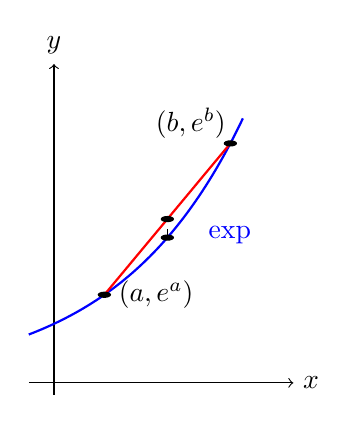
\begin{tikzpicture}[xscale=1.6,yscale=0.75]
\draw[->] (-0.2,0) -- (1.9,0) node[right] {$x$};
\draw[->] (0,-0.2) -- (0,5.4) node[above] {$y$};
\draw[blue,thick,domain=-0.2:1.5,samples=100,smooth] plot (\x,{exp(\x)});
\draw[red,thick] (0.4,{exp(0.4)}) -- (1.4,{exp(1.4)});
\fill (0.4,{exp(0.4)}) circle (1.5pt) node[right, inner sep=5pt] {$(a,e^a)$};
\fill (1.4,{exp(1.4)}) circle (1.5pt) node[above left, inner sep=1.5pt] {$(b,e^b)$};
\fill (0.9,{(exp(0.4)+exp(1.4))/2}) circle (1.5pt);
\fill (0.9,{exp(0.9)}) circle (1.5pt);
\draw[dashed] (0.9,{exp(0.9)}) -- (0.9,{(exp(0.4)+exp(1.4))/2});
\node[blue,anchor=west] at (1.15,2.5) {$\exp$};
\end{tikzpicture}
\caption{Convexity of $\exp $: the chord joining $(a,e^{a})$ and $(b,e^{b})$
lies above the graph, in particular above the midpoint.}
\label{fig:convex-exp}
\end{figure}

\begin{enumerate}
\item \underline{Positivity:}\label{Positivity} 
\begin{equation}
\forall x\in \mathbb{R}:\text{ }\exp (x)>0\text{.}
\end{equation}

\item M\underline{ultiplicativity:}\label{Multiplicativity} 
\begin{equation}
\forall x\in \mathbb{R},\forall y\in \mathbb{R}:\text{ }\exp (x+y)=\exp
(x)\exp (y).
\end{equation}

\item \underline{The identity:}\label{identity} 
\begin{equation}
\forall x\in \mathbb{R},\forall t\in \lbrack 0,1]:\text{ }\exp (tx)=(\exp
x)^{t}.
\end{equation}

\item \underline{Uniform convergence on every bounded interval: }
\end{enumerate}

\begin{quotation}
\label{Uniformconvergence}For $R\in \R_{>0}$, define a finite real 
\begin{equation*}
M_{n}(R):=\sup_{x\in [-R,R]}\Bigl|\exp (x)-\sum_{k=0}^{n}\frac{x^{k}}{k!}%
\Bigr|\qquad (n\in \N).
\end{equation*}
The function under the supremum is continuous on $[-R,R]$, so $M_n(R)$ is a
finite real.

Then: 
\begin{equation*}
\forall R\in \R_{>0},\ \forall \varepsilon \in \R_{>0},\ \exists N\in \N,\
\forall n\in \N:\quad n\geq N\Rightarrow M_{n}(R)<\varepsilon .
\end{equation*}%
A finite modulus is supplied by the tail bound 
\begin{equation*}
\forall R\in \R_{>0},\ \forall x\in [-R,R],\ \forall n\in \N:\quad
n+2>R\Rightarrow \Bigl|\exp (x)-\sum_{k=0}^{n}\frac{x^{k}}{k!}\Bigr|\leq 
\frac{R^{n+1}}{(n+1)!}\Bigl(1-\frac{R}{n+2}\Bigr)^{-1}.
\end{equation*}
Indeed, if $N$ is chosen so that for every $n\ge N$ 
\begin{equation*}
\frac{R^{n+1}}{(n+1)!}<\frac{\varepsilon}{2} \quad\text{and}\quad \Bigl(1-%
\frac{R}{n+2}\Bigr)^{-1}<2,
\end{equation*}
then $M_{n}(R)<\varepsilon$ for every $n\ge N$.

\noindent These are established in the constructive setting in
Bishop--Bridges \cite{BishopBridges1985} and elsewhere.

Constructive inequalities of means are treated in \cite{Kawakubo2026}.%
\newline
\noindent The ten proofs are organised as follows:
\end{quotation}

\begin{itemize}
\item \Cref{sec:constructive} collects the three constructive proofs (AM--GM%
\comma direct series plus translation, midpoint convexity).

\item \Cref{sec:classical} collects the three classical differential proofs
(second derivative\comma first derivative monotone\comma supporting line).

\item \Cref{sec:further} collects three further proofs (limit definition
with Bernoulli\comma inverse of the concave logarithm\comma and the pointer
to Lean).

\item \Cref{sec:lean} gives the detailed adaptation of the Lean's proof.

\item \Cref{sec:summary} summarises the ten routes in tabular form and
re-classifies each in second-order arithmetic.
\end{itemize}

\begin{definition}
For $n\in \mathbb{N}$ and $x\in \mathbb{R}$, set 
\begin{equation}
S_{n}(x):=\sum_{k=0}^{n}\frac{x^{k}}{k!}.
\end{equation}%
The exponential $\exp x$ is the unique real $L$ satisfying 
\begin{equation}
\forall \varepsilon >0\ \exists N\in \mathbb{N}\ \forall n\geq
N:|L-S_{n}(x)|<\varepsilon .
\end{equation}%
For $R\geq 0$, set $T_{n}(R):=\sum_{k=n+1}^{\infty }R^{k}/k!$.
\end{definition}

\begin{definition}[Convexity and strict convexity]
Let $I\subseteq \mathbb{R}$ be an interval and $f:I\rightarrow \mathbb{R}$.
Define 
\begin{equation}
\func{Conv}(f,I)\ \Longleftrightarrow \ \forall x,y\in I\ \forall t\in
\lbrack 0,1]:f(tx+(1-t)y)\leq tf(x)+(1-t)f(y).
\end{equation}%
Define 
\begin{equation*}
\begin{aligned} \operatorname{StrictConv}(f,I)\ \Longleftrightarrow\
&\operatorname{Conv}(f,I)\ \wedge\\ &\forall x,y\in I\ \forall t\in(0,1):\
x\ne y\ \Longrightarrow\ f(tx+(1-t)y)<tf(x)+(1-t)f(y). \end{aligned}
\end{equation*}%
For the constructive strict version, replace $x\neq y$ by $|x-y|>0$.
\end{definition}

\begin{definition}[Compact-uniform continuity modulus]
For a compact interval $J\subseteq I$ and $f:I\rightarrow \mathbb{R}$, a
modulus is a function $\mu _{J}:\mathbb{N}\rightarrow \mathbb{N}$ such that 
\begin{equation}
\forall k\in \mathbb{N}\ \forall x,y\in J:\quad |x-y|<2^{-\mu _{J}(k)}\
\Longrightarrow \ |f(x)-f(y)|<2^{-k}.
\end{equation}
\end{definition}

\begin{definition}[Derivative]
Let $I\subseteq \mathbb{R}$ be open and $x\in I$. Define $f^{\prime }(x)=L$
by 
\begin{equation}
\forall \varepsilon >0\ \exists \delta >0\ \forall h\in \mathbb{R}:\quad %
\bigl(0<|h|<\delta \ \wedge \ x+h\in I\bigr)\Longrightarrow \left\vert \frac{%
f(x+h)-f(x)}{h}-L\right\vert <\varepsilon .
\end{equation}
\end{definition}

\begin{definition}[$C^{k}$ on an open interval]
For an open interval $I$, define $f\in C^{k}(I)$ if there exist continuous
functions $g_{0},\ldots ,g_{k}:I\rightarrow \mathbb{R}$ such that 
\begin{equation}
g_{0}=f,\qquad g_{j}^{\prime }(x)=g_{j+1}(x)\quad (x\in I,\ 0\leq j<k).
\end{equation}
\end{definition}

\begin{definition}[Cauchy codes and base theories]
A fast Cauchy code for a real is a sequence $q:\mathbb{N}\rightarrow \mathbb{%
Q}$ with 
\begin{equation}
|q_{m}-q_{n}|\leq 2^{-n}\qquad (m\geq n).
\end{equation}%
Two such codes represent the same real if their difference tends to zero. On
a rational compact interval, a modulated continuous-function code consists
of coherent rational value approximations on rational inputs and a modulus
as in Definition~\ref{defi:conv-cont}; evaluation at real inputs is by
Cauchy approximation. On open domains use compatible codes on a compact
exhaustion. Set 
\begin{equation*}
\begin{aligned} \mathsf{RCA}_0&:=\text{basic second-order arithmetic}
+\Delta^0_1\text{-comprehension}+\Sigma^0_1\text{-induction},\\
\mathsf{WKL}_0&:=\mathsf{RCA}_0+\mathsf{WKL}, \end{aligned}
\end{equation*}%
where $\mathsf{WKL}$ asserts that every infinite binary tree has an infinite
path. Real quantifiers in coded statements range over valid Cauchy codes.
\end{definition}



\label{sec:constructive}

\begin{theorem}
\label{thm:uniform-tail} The exponential exists uniquely. {\scriptsize 
\begin{equation}
\forall R\in 
%TCIMACRO{\U{211d} }%
%BeginExpansion
\mathbb{R}
%EndExpansion
_{>0},\text{ }\forall n\in 
%TCIMACRO{\U{2115} }%
%BeginExpansion
\mathbb{N}
%EndExpansion
,\text{ }\forall x\in 
%TCIMACRO{\U{211d} }%
%BeginExpansion
\mathbb{R}
%EndExpansion
,\text{ }|x|\leq R<n+2\Rightarrow \text{ }|\exp x-S_{n}(x)|\leq T_{n}(R)\leq 
\frac{R^{n+1}}{(n+1)!}\left( 1-\frac{R}{n+2}\right) ^{-1}.
\label{eq:uniform-tail}
\end{equation}%
} For each fixed $R$, the convergence has a computable modulus.
\end{theorem}

\begin{proof}
\medskip

\noindent {\ \centering \setlength{\tabcolsep}{3pt}\renewcommand{%
\arraystretch}{1.0}\parskip=0pt 
\begin{tabular}{|@{}p{0.06\linewidth}p{0.61\linewidth}p{0.29\linewidth}}
\hline
1 & $R>0,\quad |x|\leq R,\quad \varepsilon >0$ & Arbitrary parameters;
assumption. \\ \hline
\medskip 2 & \medskip $B\in \mathbb{N},\quad B\geq \max (1,R)$ & Archimedean
bound, 1. \\ 
\end{tabular}%
}\vspace{-5pt} \noindent

{\ \centering\setlength{\tabcolsep}{3pt}\renewcommand{\arraystretch}{1.0}%
\parskip=0pt 
\begin{tabular}{|@{}p{0.06\linewidth}p{0.61\linewidth}p{0.29\linewidth}}
\hline
3 & \medskip $b_{n}:=\dfrac{B^{n+1}}{(n+1)!}$\medskip & Definition. \\ \hline
\medskip 4 & \medskip $n+2\geq 2B$ & Assumption. \\ 
\end{tabular}%
} \vspace{-5pt} \noindent

{\ \centering\setlength{\tabcolsep}{3pt}\renewcommand{\arraystretch}{1.0}%
\parskip=0pt 
\begin{tabular}{|@{}p{0.06\linewidth}p{0.61\linewidth}p{0.29\linewidth}}
\hline
5 & $b_{n+1}/b_{n}=B/(n+2)\leq 1/2$ & Arithmetic, 2--4. \\ \hline
\medskip 6 & \medskip $\exists N:\ N+2\geq 2B\ \wedge \ b_{N}<\varepsilon /2$
& Geometric decay, 3--5; discharge 4. \\  
\end{tabular}%
} \vspace{-5pt} \noindent \noindent

{\ \centering\setlength{\tabcolsep}{3pt}\renewcommand{\arraystretch}{1.0}%
\parskip=0pt 
\begin{tabular}{|@{}p{0.06\linewidth}p{0.61\linewidth}p{0.29\linewidth}}
\hline
7 & $\begin{aligned}m>n\ge N\ \Longrightarrow
|S_m(x)-S_n(x)|\le2b_n<\varepsilon\end{aligned}$ & Finite geometric
majorant, 5--6. \\ \hline
\medskip 8 & \medskip $\exists L\in \mathbb{R}:\ S_{n}(x)\longrightarrow L$
& Modulated Cauchy construction, 7. \\ 
\end{tabular}%
} \vspace{-5pt} \noindent \noindent

{\ \centering\setlength{\tabcolsep}{3pt}\renewcommand{\arraystretch}{1.0}%
\parskip=0pt 
\begin{tabular}{|@{}p{0.06\linewidth}p{0.61\linewidth}p{0.29\linewidth}}
\hline
9 & $\begin{aligned}n+2>R\ \Longrightarrow |L-S_n(x)|\le T_n(R)
\le\dfrac{R^{n+1}}{(n+1)!}(1-R/(n+2))^{-1}\end{aligned}$ & Geometric tail
estimate; non-strict limit, 7--8. \\ \hline
\medskip 10 & \medskip $S_{n}(x)\rightarrow L\ \wedge \ S_{n}(x)\rightarrow
L^{\prime }$ & Assumption for uniqueness. \\ 
\end{tabular}%
} \vspace{-5pt} \noindent \noindent

{\ \centering\setlength{\tabcolsep}{3pt}\renewcommand{\arraystretch}{1.0}%
\parskip=0pt 
\begin{tabular}{|@{}p{0.06\linewidth}p{0.61\linewidth}p{0.29\linewidth}}
\hline
11 & $\eta >0$ & Arbitrary positive tolerance. \\ \hline
12 & $\exists n:\ |L-S_{n}(x)|<\eta /2\ \wedge \ |L^{\prime }-S_{n}(x)|<\eta
/2$ & Limit definition, 10--11. \\ 
\end{tabular}%
} \vspace{-5pt} \noindent \noindent

{\ \centering\setlength{\tabcolsep}{3pt}\renewcommand{\arraystretch}{1.0}%
\parskip=0pt 
\begin{tabular}{|@{}p{0.06\linewidth}p{0.61\linewidth}p{0.29\linewidth}}
\hline
13 & $|L-L^{\prime }|<\eta $ & Triangle inequality, 12. \\ \hline
\medskip 14 & \medskip $L=L^{\prime }$ & Arbitrary-tolerance criterion,
11--13. \\ 
\end{tabular}%
} \vspace{-5pt} \noindent \noindent

{\ \centering\setlength{\tabcolsep}{3pt}\renewcommand{\arraystretch}{1.0}%
\parskip=0pt 
\begin{tabular}{|@{}p{0.06\linewidth}p{0.61\linewidth}p{0.29\linewidth}}
\hline
15 & $\exists !L:\ S_{n}(x)\rightarrow L$ & Existence 8; uniqueness 10--14.
\\ \hline
16 & \medskip $\begin{gathered}\forall x\in\mathbb R,\, \exists!L:\
S_n(x)\to L,\, \forall R>0,\, \forall x\in[-R,R],\, \forall n: \\ n+2>R\
\Longrightarrow |e^x-S_n(x)|\le
T_n(R)\le\dfrac{R^{n+1}}{(n+1)!}(1-R/(n+2))^{-1}\end{gathered}$ \medskip & 
Discharge 1; generalization, 6--15. \\ \hline
\end{tabular}%
}
\end{proof}

\begin{theorem}[Series foundations]
\label{lem:series-foundations} The power series defines a continuous
positive function on $\mathbb{R}$ with $\exp 0=1$ and 
\begin{equation*}
\forall x\in 
%TCIMACRO{\U{211d} }%
%BeginExpansion
\mathbb{R}
%EndExpansion
,\forall y\in 
%TCIMACRO{\U{211d} }%
%BeginExpansion
\mathbb{R}
%EndExpansion
:\exp (x+y)=\exp x\exp y.
\end{equation*}
\begin{equation*}
\forall h\in 
%TCIMACRO{\U{211d} }%
%BeginExpansion
\mathbb{R}
%EndExpansion
_{\geq 0}:\text{ }\exp h\geq 1+h.
\end{equation*}%
\begin{equation}
\forall B\in 
%TCIMACRO{\U{211d} }%
%BeginExpansion
\mathbb{R}
%EndExpansion
_{\geq 1},\forall u\in \lbrack -B,B],\text{ },\forall v\in \lbrack -B,B]:%
\text{ }|\exp u-\exp v|\leq \exp (B)|u-v|  \label{eq:exp-lipschitz}
\end{equation}
\end{theorem}

\begin{proof}
\smallskip \noindent {\ \setlength{\tabcolsep}{3pt}\renewcommand{%
\arraystretch}{1.18}}

{\ \centering\setlength{\tabcolsep}{3pt}\renewcommand{\arraystretch}{1.0}%
\parskip=0pt 
\begin{tabular}{|@{}p{0.06\linewidth}p{0.61\linewidth}p{0.29\linewidth}}
\hline
1 & $B\ge1,\quad u,v\in[-B,B]$ & Arbitrary parameters. \\ \hline
2 & $|u^k-v^k|\le kB^{k-1}|u-v|\quad(k\ge1)$ & Difference-of-powers
identity; triangle inequality. \\ 
\end{tabular}%
} \vspace{-5pt} \noindent

\noindent {\ \centering\setlength{\tabcolsep}{3pt}\renewcommand{%
\arraystretch}{1.0}\parskip=0pt 
\begin{tabular}{|@{}p{0.06\linewidth}p{0.61\linewidth}p{0.29\linewidth}}
\hline
3 & $|S_n(u)-S_n(v)|\le |u-v|S_{n-1}(B)\quad(n\ge1)$ & Sum 2 with weights $%
1/k!$. \\ \hline
4 & $|e^u-e^v|\le e^B|u-v|$ & Non-strict limit, 3; Theorem~\ref%
{thm:uniform-tail}. \\ 
\end{tabular}
} \vspace{-5pt} \noindent

\noindent {\ \centering\setlength{\tabcolsep}{3pt}\renewcommand{%
\arraystretch}{1.0}\parskip=0pt 
\begin{tabular}{|@{}p{0.06\linewidth}p{0.61\linewidth}p{0.29\linewidth}}
\hline
5 & $\exp\text{ is continuous on }\mathbb{R}$ & Arbitrary bounded interval,
1--4. \\ \hline
6 & $x,y\in\mathbb{R},\quad |x|\le R,\ |y|\le S$ & Arbitrary parameters and
integer bounds. \\ 
\end{tabular}
} \vspace{-5pt} \noindent

\noindent {\ \centering\setlength{\tabcolsep}{3pt}\renewcommand{%
\arraystretch}{1.0}\parskip=0pt 
\begin{tabular}{|@{}p{0.06\linewidth}p{0.61\linewidth}p{0.29\linewidth}}
\hline
7 & $S_N(x+y)=\displaystyle\sum_{i+j\le N}\frac{x^iy^j}{i!j!}$ & Finite
binomial identity. \\ \hline
8 & \medskip \medskip $\begin{aligned}\sum_{i+j>2m}\frac{|x|^i|y|^j}{i!j!}
\le T_m(R)e^S+e^R T_m(S)\to0\end{aligned}$ & Union bound $i>m$ or $j>m$;
absolute tails. \\  
\end{tabular}%
} \vspace{-5pt} \noindent

\noindent {\ \centering\setlength{\tabcolsep}{3pt}\renewcommand{%
\arraystretch}{1.0}\parskip=0pt 
\begin{tabular}{|@{}p{0.06\linewidth}p{0.61\linewidth}p{0.29\linewidth}}
\hline
9 & $e^{x+y}=e^xe^y$ & Modulated Cauchy product, 7--8. \\ \hline
10 & $\forall x,y\in\mathbb{R}:\ e^{x+y}=e^xe^y$ & Generalization, 6--9. \\ 
\end{tabular}
} \vspace{-5pt} \noindent

\noindent {\ \centering\setlength{\tabcolsep}{3pt}\renewcommand{%
\arraystretch}{1.0}\parskip=0pt 
\begin{tabular}{|@{}p{0.06\linewidth}p{0.61\linewidth}p{0.29\linewidth}}
\hline
11 & $x\in\mathbb{R}$ & Arbitrary parameter. \\ \hline
12 & $e^0=1,\quad e^xe^{-x}=1,\quad e^x=(e^{x/2})^2\ge0$ & Definition of
series; 10; square non-negativity. \\ 
\end{tabular}%
} \vspace{-5pt} \noindent

\noindent {\ \centering\setlength{\tabcolsep}{3pt}\renewcommand{%
\arraystretch}{1.0}\parskip=0pt 
\begin{tabular}{|@{}p{0.06\linewidth}p{0.61\linewidth}p{0.29\linewidth}}
\hline
13 & $C\in\mathbb{Q},\quad C>\max(0,e^{-x})$ & Rational upper bound from the
tail estimate. \\ \hline
14 & $1=e^xe^{-x}\le Ce^x$ & Order multiplication, 12--13. \\ 
\end{tabular}%
} \vspace{-5pt} \noindent

\noindent {\ \centering\setlength{\tabcolsep}{3pt}\renewcommand{%
\arraystretch}{1.0}\parskip=0pt 
\begin{tabular}{|@{}p{0.06\linewidth}p{0.61\linewidth}p{0.29\linewidth}}
\hline
15 & $e^x\ge1/C>0$ & Divide by $C>0$, 14. \\ \hline
16 & $\forall x\in\mathbb{R}:\ e^x>0$ & Generalization, 11--15. \\ 
\end{tabular}%
} \vspace{-5pt}

\noindent {\ \centering\setlength{\tabcolsep}{3pt}\renewcommand{%
\arraystretch}{1.0}\parskip=0pt 
\begin{tabular}{|@{}p{0.06\linewidth}p{0.61\linewidth}p{0.29\linewidth}}
\hline
17 & $h\ge0,\quad n\ge1$ & Arbitrary parameters; assumptions. \\ \hline
18 & $S_n(h)\ge1+h$ & Non-negative terms in the finite series. \\ 
\end{tabular}%
} \vspace{-5pt}

\noindent {\ \centering\setlength{\tabcolsep}{3pt}\renewcommand{%
\arraystretch}{1.0}\parskip=0pt 
\begin{tabular}{|@{}p{0.06\linewidth}p{0.61\linewidth}p{0.29\linewidth}}
\hline
19 & $e^h\ge1+h$ & Non-strict limit, 18. \\ \hline
20 & $\forall h\ge0:\ e^h\ge1+h$ & Discharge and generalization, 17--19. \\ 
\hline
\end{tabular}%
}
\end{proof}

\begin{theorem}[Effective inverse construction]
\label{lem:log-construction} {\setstretch{1.8} The power-series exponential
is a strictly increasing bijection from $\mathbb{R}$ onto $\mathbb{R}_{>0}$. 
}%
\begin{equation*}
\begin{gathered}\exp:\mathbb R\overset{\sim}{\longrightarrow}\mathbb
R_{>0},\\
\log\circ\exp=\mathrm{id}_{\R},\quad\exp\circ\log=\mathrm{id}_{\R_{>0}}.%
\end{gathered}
\end{equation*}

{Its inverse $\log $ can be constructed by a modulated rational-interval
procedure without an exact intermediate value principle or any convexity
theorem, such that: } 
\begin{equation*}
\forall a\in 
%TCIMACRO{\U{211d} }%
%BeginExpansion
\mathbb{R}
%EndExpansion
_{>0},\text{ }\forall t\in 
%TCIMACRO{\U{211d} }%
%BeginExpansion
\mathbb{R}
%EndExpansion
:a^{t}:=\exp (t\log a).
\end{equation*}

And,%
\begin{equation*}
\forall x\in 
%TCIMACRO{\U{211d} }%
%BeginExpansion
\mathbb{R}
%EndExpansion
,\forall t\in 
%TCIMACRO{\U{211d} }%
%BeginExpansion
\mathbb{R}
%EndExpansion
:\text{ }\exp (tx)=(\exp x)^{t}.
\end{equation*}
\end{theorem}

\begin{proof}
\smallskip \noindent {\ \setlength{\tabcolsep}{3pt}\renewcommand{%
\arraystretch}{1.18}}

{\ \centering\setlength{\tabcolsep}{3pt}\renewcommand{\arraystretch}{1.0}%
\parskip=0pt 
\begin{tabular}{|@{}p{0.06\linewidth}p{0.61\linewidth}p{0.29\linewidth}}
\hline
1 & $p<q$ & Arbitrary real parameters; assumption. \\ \hline
2 & $e^q-e^p=e^p(e^{q-p}-1)\ge e^p(q-p)>0$ & Theorem~\ref%
{lem:series-foundations}, positivity and multiplication. \\ 
\end{tabular}%
} \vspace{-5pt}

\noindent {\ \centering\setlength{\tabcolsep}{3pt}\renewcommand{%
\arraystretch}{1.0}\parskip=0pt 
\begin{tabular}{|@{}p{0.06\linewidth}p{0.61\linewidth}p{0.29\linewidth}}
\hline
3 & $\exp\text{ is strictly increasing}$ & Discharge and generalization,
1--2. \\ \hline
4 & $a>0$ & Arbitrary target. \\  
\end{tabular}%
} \vspace{-5pt}

\noindent {\ \centering\setlength{\tabcolsep}{3pt}\renewcommand{%
\arraystretch}{1.0}\parskip=0pt 
\begin{tabular}{|@{}p{0.06\linewidth}p{0.61\linewidth}p{0.29\linewidth}}
\hline
5 & $\begin{gathered}0<\ell<a<A,\quad M\in\mathbb N_{\ge1},\quad
1+M>A,\quad(1+M)^{-1}<\ell\end{gathered}$ & Rational bounds and Archimedean
search, 4. \\ \hline
6 & $e^{-M}\le(1+M)^{-1}<a<1+M\le e^M$ & Positive-series bound and
multiplication. \\ 
\end{tabular}%
} \vspace{-5pt}

\noindent {\ \centering\setlength{\tabcolsep}{3pt}\renewcommand{%
\arraystretch}{1.0}\parskip=0pt 
\begin{tabular}{|@{}p{0.06\linewidth}p{0.61\linewidth}p{0.29\linewidth}}
\hline
7 & $C\in\mathbb{Q},\quad C>e^M,\quad c:=1/C>0$ & Effective series bound. \\ 
\hline
8 & \medskip $e^q-e^p\ge c(q-p)\quad(-M\le p<q\le M)$ & 2--3, 7; $e^p\ge
e^{-M}\ge c$. \\ 
\end{tabular}%
} \vspace{-5pt}

\noindent {\ \centering\setlength{\tabcolsep}{3pt}\renewcommand{%
\arraystretch}{1.0}\parskip=0pt 
\begin{tabular}{|@{}p{0.06\linewidth}p{0.61\linewidth}p{0.29\linewidth}}
\hline
9 & $e^l<a<e^u,\quad l,u\in\mathbb{Q}\cap[-M,M]$ & Bracket invariant;
initially 6. \\ \hline
10 & $w=u-l,\quad p=l+w/3,\quad q=l+2w/3$ & Definitions. \\ 
\end{tabular}%
} \vspace{-5pt}

\nointerlineskip\noindent {\ \centering\setlength{\tabcolsep}{3pt}\renewcommand{%
\arraystretch}{1.0}\parskip=0pt 
\begin{tabular}{|@{}p{0.06\linewidth}p{0.61\linewidth}p{0.29\linewidth}}
\hline
11 & $\begin{gathered}E_p,E_q,a_0\in\mathbb Q, |E_p-e^p|<cw/24,\,
|E_q-e^q|<cw/24,\,\\ |a_0-a|<cw/24\end{gathered}$ & Cauchy
approximations, 7--10. \\ \hline
12 & $d_1:=a_0-E_p,\quad d_2:=E_q-a_0$ & Definitions. \\ 
\end{tabular}%
} \vspace{-5pt}

\nointerlineskip\noindent { \centering\setlength{\tabcolsep}{3pt}\renewcommand{%
\arraystretch}{1.0}\parskip=0pt 
\begin{tabular}{|@{}p{0.06\linewidth}p{0.61\linewidth}p{0.29\linewidth}}
\hline
13 & $d_1+d_2=E_q-E_p>cw/4$ & Separation 8; error estimate
11. \\ \hline
14 & $d_1>cw/8$ & Decidable rational test: first branch. \\ 
\end{tabular}%
} \vspace{-5pt}

\nointerlineskip\noindent {\ \centering\setlength{\tabcolsep}{3pt}\renewcommand{%
\arraystretch}{1.0}\parskip=0pt 
\begin{tabular}{|@{}p{0.06\linewidth}p{0.61\linewidth}p{0.29\linewidth}}
\hline
15 & $a-e^p>cw/24>0$ & Error bound 11 and 14. \\ \hline
16 & $e^p<a<e^u,\quad u-p=2w/3$ & 9--10, 15; keep $[p,u]$. \\ 
\end{tabular}%
} \vspace{-5pt}

\noindent {\ \centering\setlength{\tabcolsep}{3pt}\renewcommand{%
\arraystretch}{1.0}\parskip=0pt 
\begin{tabular}{|@{}p{0.06\linewidth}p{0.61\linewidth}p{0.29\linewidth}}
\hline
17 & $d_1\le cw/8$ & Complementary rational branch. \\ \hline
18 & $d_2>cw/8,\quad e^q-a>cw/24>0$ & 11--13, 17. \\ 
\end{tabular}%
} \vspace{-5pt}

\noindent {\ \centering\setlength{\tabcolsep}{3pt}\renewcommand{%
\arraystretch}{1.0}\parskip=0pt 
\begin{tabular}{|@{}p{0.06\linewidth}p{0.61\linewidth}p{0.29\linewidth}}
\hline
19 & $e^l<a<e^q,\quad q-l=2w/3$ & 9--10, 18; keep $[l,q]$. \\ \hline
20 &  $\exists[l^{\prime },u^{\prime }]\subseteq[l,u]:\ %
\begin{gathered}e^{l'}<a<e^{u'},\quad u'-l'=2w/3\end{gathered}$ & Rational
cases, 14--16 and 17--19. \\ 
\end{tabular}%
} \vspace{-5pt}

\noindent {\ \centering\setlength{\tabcolsep}{3pt}\renewcommand{%
\arraystretch}{1.0}\parskip=0pt 
\begin{tabular}{|@{}p{0.06\linewidth}p{0.61\linewidth}p{0.29\linewidth}}
\hline
21 & $\begin{gathered}{}[l_j,u_j]\text{ nested},\quad
u_j-l_j=2M(2/3)^j,\quad e^{l_j}<a<e^{u_j}\end{gathered}$ & Effective
recursion from 6 and 9--20. \\ \hline
22 & $\exists y:\ l_j\to y\ \land\ u_j\to y\ \land\ e^y=a$ & Cauchy modulus
21; continuity and squeeze. \\ 
\end{tabular}%
} \vspace{-5pt}

\noindent {\ \centering\setlength{\tabcolsep}{3pt}\renewcommand{%
\arraystretch}{1.0}\parskip=0pt 
\begin{tabular}{|@{}p{0.06\linewidth}p{0.61\linewidth}p{0.29\linewidth}}
\hline
23 & $|p-q|\le C|e^p-e^q|\quad(p,q\in[-M,M])$ & Rational order cases in 8;
extend by continuity. \\ \hline
24 & $\exists! y:\ e^y=a$ & Existence 22; uniqueness 23 on a common bracket.
\\ 
\end{tabular}%
} \vspace{-5pt}

\noindent {\ \centering\setlength{\tabcolsep}{3pt}\renewcommand{%
\arraystretch}{1.0}\parskip=0pt 
\begin{tabular}{|@{}p{0.06\linewidth}p{0.61\linewidth}p{0.29\linewidth}}
\hline
25 & $\log a:=y,\quad e^{\log a}=a$ & Unique inverse definition, 24. \\ 
\hline
26 & $\log(e^x)=x\quad(x\in\mathbb{R})$ & Uniqueness 24--25; arbitrary
target. \\ 
\end{tabular}%
} \vspace{-5pt}

\noindent {\ \centering\setlength{\tabcolsep}{3pt}\renewcommand{%
\arraystretch}{1.0}\parskip=0pt 
\begin{tabular}{|@{}p{0.06\linewidth}p{0.61\linewidth}p{0.29\linewidth}}
\hline
27 & $0<a<b,\quad p=\log a,\ q=\log b$ & Arbitrary positive inputs; common
bracket. \\ \hline
28 & $0<b-a\le D\max(q-p,0),\quad D\in\mathbb{Q},\ D>e^M$ & Rational order
cases; Lipschitz estimate; continuity. \\ 
\end{tabular}%
} \vspace{-5pt}

\noindent {\ \centering\setlength{\tabcolsep}{3pt}\renewcommand{%
\arraystretch}{1.0}\parskip=0pt 
\begin{tabular}{|@{}p{0.06\linewidth}p{0.61\linewidth}p{0.29\linewidth}}
\hline
29 & $q-p>0$ & Positive-gap order consequence, 28. \\ \hline
30 & $\log\text{ is strictly increasing}$ & Discharge and generalization,
27--29. \\ 
\end{tabular}%
} \vspace{-5pt}

\noindent {\ \centering\setlength{\tabcolsep}{3pt}\renewcommand{%
\arraystretch}{1.0}\parskip=0pt 
\begin{tabular}{|@{}p{0.06\linewidth}p{0.61\linewidth}p{0.29\linewidth}}
\hline
31 & $|\log a-\log b|\le C|a-b|$ & 23, 25 on a common compact positive input
interval. \\ \hline
32 & $\log\text{ has compact-uniform moduli}$ & Rational bound $C$, 31;
generalization. \\ 
\end{tabular}%
} \vspace{-5pt}

\noindent {\ \centering\setlength{\tabcolsep}{3pt}\renewcommand{%
\arraystretch}{1.0}\parskip=0pt 
\begin{tabular}{|@{}p{0.06\linewidth}p{0.61\linewidth}p{0.29\linewidth}}
\hline
33 & $a>0,\quad t\in\mathbb{R},\quad a^t:=e^{t\log a}$ & Real-power
definition. \\ \hline
34 & $(e^x)^t=e^{t\log(e^x)}=e^{tx}$ & Substitution, 26 and 33. \\ 
\end{tabular}%
} \vspace{-5pt}

\noindent {\ \centering\setlength{\tabcolsep}{3pt}\renewcommand{%
\arraystretch}{1.0}\parskip=0pt 
\begin{tabular}{|@{}p{0.06\linewidth}p{0.61\linewidth}p{0.29\linewidth}}
\hline
35 & $(a^{m/n})^n=a^m\quad(m\in\mathbb{N},\ n\ge1)$ & Multiplicativity; 33.
\\ \hline
36 & $a^{m/n}=\sqrt[n]{a^m},\quad t\mapsto a^t\text{ continuous}$ & 
Positive-root uniqueness; composition with $\exp$. \\ 
\end{tabular}%
} \vspace{-7pt}

\noindent {\ \centering\setlength{\tabcolsep}{3pt}\renewcommand{%
\arraystretch}{2.0}\parskip=0pt 
\begin{tabular}{|@{}p{0.06\linewidth}p{0.61\linewidth}p{0.29\linewidth}}
\hline
37 & $\begin{gathered}\exp:\mathbb R\overset{\sim}{\longrightarrow}\mathbb
R_{>0},\\
\log\circ\exp=\mathrm{id}_{\R},\quad\exp\circ\log=\mathrm{id}_{\R_{>0}},\\
(e^x)^t=e^{tx}\end{gathered}$ & Generalization, 24--36; continuity moduli
from 31--32. \\ \hline
\end{tabular}%
}
\end{proof}
\section{Constructive proofs}
\subsection{ Weighted AM--GM (First proof)}

\begin{lemma}[Weighted AM--GM\comma two variables]
\label{lem:weighted-amgm} For every $a\in\R_{>0}$, every $b\in\R_{>0}$, and
every $t\in[0,1]$,

\begin{ineq}
\label{eq:weighted-amgm} a^{t}\,b^{1-t}\ \le\ t\,a+(1-t)\,b,
\end{ineq}

where $a^{t}$ and $b^{1-t}$ denote the real powers $\mathtt{Real.rpow}\ a\ t$
and $\mathtt{Real.rpow}\ b\ (1-t)$.
\end{lemma}

\begin{proof}
\noindent\underline{{\large \emph{Rational case:}}}

\noindent Suppose $t=m/n$ with $m,n\in \N$, $0\leq m\leq n$, $n\geq 1$.

Applying the ordinary AM--GM inequality (see \cite{Hardy1952}) to the $n$
positive numbers consisting of $m$ copies of $a$ and $n-m$ copies of $b$
gives 
\begin{equation*}
\bigl(a^{m}b^{n-m}\bigr)^{1/n}\leq \frac{ma+(n-m)b}{n}.
\end{equation*}%
The left-hand side equals 
\begin{equation*}
a^{m/n}b^{(n-m)/n}=a^{t}b^{1-t},
\end{equation*}%
and the right-hand side equals 
\begin{equation*}
\frac{m}{n}a+\frac{n-m}{n}b=ta+(1-t)b.
\end{equation*}%
Hence \cref{eq:weighted-amgm} holds whenever $t$ is rational.

\noindent\underline{{\large \emph{Real case:}}}

\noindent Fix $t\in [0,1]$ and $\varepsilon >0$.

The maps $s\mapsto a^{s}b^{1-s}$ and $s\mapsto sa+(1-s)b$ are continuous on $%
[0,1]$, so there is $\delta >0$ such that, for every $t^{\prime }\in
[0,1]\cap \Q$ with $|t-t^{\prime }|<\delta $, 
\begin{equation*}
\bigl|a^{t}b^{1-t}-a^{t^{\prime }}b^{1-t^{\prime }}\bigr|<\tfrac{\varepsilon 
}{2},\qquad \bigl|(ta+(1-t)b)-(t^{\prime }a+(1-t^{\prime })b)\bigr|<\tfrac{%
\varepsilon }{2}.
\end{equation*}%
Choose such a $t^{\prime }$. By the rational case, $a^{t^{\prime
}}b^{1-t^{\prime }}\leq t^{\prime }a+(1-t^{\prime })b$.

Combining, 
\begin{equation*}
a^{t}b^{1-t}<a^{t^{\prime }}b^{1-t^{\prime }}+\tfrac{\varepsilon }{2}\leq
t^{\prime }a+(1-t^{\prime })b+\tfrac{\varepsilon }{2}<ta+(1-t)b+\varepsilon .
\end{equation*}%
Since $\varepsilon >0$ was arbitrary, \cref{eq:weighted-amgm} follows.
\end{proof}

\begin{theorem}[Convexity via AM--GM]
\label{thm:amgm} For every $x\in\R$, every $y\in\R$, and every $t\in[0,1]$,

\begin{ineq}
\label{eq:convex-amgm} \exp\bigl(tx+(1-t)y\bigr)\ \le\ t\,\exp x+(1-t)\,\exp
y .
\end{ineq}
\end{theorem}

\begin{proof}
\noindent By multiplicativity and the identity $\exp(tx)=(\exp x)^{t}$ (see 
\texttt{Pos:ExpPow} in \S \ref{sec:convexity-postulates}; for real $t$ it
follows from the rational case together with continuity of both $t\mapsto
\exp(tx)$ and $t\mapsto (\exp x)^{t}$), we get 
\begin{equation*}
\exp \bigl(tx+(1-t)y\bigr)=(\exp x)^{t}(\exp y)^{1-t}.
\end{equation*}%
\noindent Apply \Cref{lem:weighted-amgm} with $a=\exp x>0$ and $b=\exp y>0$.

Then: 
\begin{equation*}
(\exp x)^{t}(\exp y)^{1-t}\leq t\exp x+(1-t)\exp y,
\end{equation*}%
which combined with the display gives \cref{eq:convex-amgm}.
\end{proof}

\subsection{Direct series on the non-negative reals (Second proof)}

\begin{lemma}[Monomial convexity on the non-negative reals]
\label{lem:monomial}

\begin{ineq}
\label{eq:monomial-convex} \forall n\in\N_{\geq 1},\ x,y\in\R_{\ge0},\
\forall t\in[0,1]:\quad \bigl(tx+(1-t)y\bigr)^{n}\ \le\
t\,x^{n}+(1-t)\,y^{n}.
\end{ineq}
\end{lemma}

\begin{proof}
\noindent\underline{{\large \emph{Base case:}}}

\noindent For $n=1$ both sides equal $tx+(1-t)y$, so %
\cref{eq:monomial-convex} holds with equality.

\noindent\underline{{\large \emph{Inductive step:}}}

\noindent Assume \cref{eq:monomial-convex} for some $n\geq 1$, and put 
\begin{equation*}
z:=tx+(1-t)y.
\end{equation*}
Since $t\in [0,1]$ and $x,y\geq 0$, we have $z\geq 0$.

Hence 
\begin{equation*}
z^{n+1}=zz^{n}\leq z\bigl(tx^{n}+(1-t)y^{n}\bigr).
\end{equation*}%
Comparing the right-hand side with the target bound 
\begin{equation*}
tx^{n+1}+(1-t)y^{n+1},
\end{equation*}%
the gap is 
\begin{equation*}
tx^{n+1}+(1-t)y^{n+1}-z\bigl(tx^{n}+(1-t)y^{n}\bigr)=t(1-t)\bigl(%
x^{n+1}+y^{n+1}-xy^{n}-x^{n}y\bigr)=t(1-t)(x-y)(x^{n}-y^{n}).
\end{equation*}%
Since $t(1-t)\geq 0$, and since $x,y\geq 0$ forces the two factors $x-y$ and 
$x^{n}-y^{n}$ to have the same sign, their product is $\geq 0$.

Therefore 
\begin{equation*}
z\bigl(tx^{n}+(1-t)y^{n}\bigr)\leq tx^{n+1}+(1-t)y^{n+1}.
\end{equation*}%
Combining with the inductive inequality gives 
\begin{equation*}
z^{n+1}\leq tx^{n+1}+(1-t)y^{n+1},
\end{equation*}%
which is \cref{eq:monomial-convex} with $n$ replaced by $n+1$.
\end{proof}

\begin{theorem}[Convexity on the non-negative reals from the series]
\label{thm:series-pos} For $N\in \N$ and $u\in \R$, put 
\begin{equation*}
S_{N}(u):=\sum_{k=0}^{N}u^{k}/k!.
\end{equation*}%
Then:

\begin{enumerate}
\item \smallskip \noindent \underline{\emph{Polynomial level :}}

\begin{ineq}
\label{eq:S_N-convex} \forall N\in \N,\forall x\in \R_{\geq 0}, \forall y\in %
\R_{\geq 0}, \forall t\in [0,1]:\, S_N(tx+(1-t)y)\ \le\
t\,S_N(x)+(1-t)\,S_N(y).
\end{ineq}

\item \smallskip \underline{\emph{\ Exponential level }:}

\begin{ineq}
\forall x\in \R_{\geq 0}, \forall y\in \R_{\geq 0}, \forall t\in [0,1]:\quad
\exp(tx+(1-t)y)\ \le\ t\,\exp x+(1-t)\,\exp y. \label{eq:convex-series-pos}
\end{ineq}
\end{enumerate}
\end{theorem}

\begin{proof}
\noindent Put 
\begin{equation*}
P_{t}(x,y):=tx+(1-t)y.
\end{equation*}%
Since $x,y\geq 0$ and $t\in [0,1]$, we have $P_{t}(x,y)\geq 0$.

\noindent \underline{{\large \emph{Proof of \cref{eq:S_N-convex} }}}

\noindent Fix $N\in \N$, $x,y\in \R_{\geq 0}$, $t\in [0,1]$.

By definition, 
\begin{equation*}
S_{N}(P_{t}(x,y))=\sum_{k=0}^{N}\frac{P_{t}(x,y)^{k}}{k!},\qquad
t\,S_{N}(x)+(1-t)\,S_{N}(y)=\sum_{k=0}^{N}\frac{t\,x^{k}+(1-t)\,y^{k}}{k!}.
\end{equation*}%
For every $k\in \N$ with $k\geq 1$, \Cref{lem:monomial} gives 
\begin{equation*}
P_{t}(x,y)^{k}\leq t\,x^{k}+(1-t)\,y^{k}.
\end{equation*}%
For $k=0$ both sides equal $1$.

Dividing by $k!$ and summing over $k=0,\dots ,N$, 
\begin{equation*}
S_{N}(P_{t}(x,y))\leq t\,S_{N}(x)+(1-t)\,S_{N}(y),
\end{equation*}%
which is \cref{eq:S_N-convex}.

\noindent \underline{{\large \emph{Proof of \cref{eq:convex-series-pos} }}}

\noindent Fix $x,y\in \R_{\geq 0}$, $t\in [0,1]$, and $\varepsilon >0$.

By the $\varepsilon $-$N$ characterisation of $\exp $ stated in the
introduction, there are $N_{1},N_{2},N_{3}\in \N$ such that, for every $N\in %
\N$, 
\begin{align*}
N\geq N_{1}\ & \Longrightarrow \ \bigl|\exp (P_{t}(x,y))-S_{N}(P_{t}(x,y))%
\bigr|<\tfrac{\varepsilon }{3}, \\
N\geq N_{2}\ & \Longrightarrow \ \bigl|\exp (x)-S_{N}(x)\bigr|<\tfrac{%
\varepsilon }{3}, \\
N\geq N_{3}\ & \Longrightarrow \ \bigl|\exp (y)-S_{N}(y)\bigr|<\tfrac{%
\varepsilon }{3}.
\end{align*}%
Set 
\begin{equation*}
N\geq N_{0},\text{ \ \ }N_{0}:=\max \{N_{1},N_{2},N_{3}\}.
\end{equation*}

Since $t\in [0,1]$, 
\begin{equation*}
\bigl|t\exp x-t\,S_{N}(x)\bigr|\leq |\exp x-S_{N}(x)|<\tfrac{\varepsilon }{3}%
,\qquad \bigl|(1-t)\exp y-(1-t)\,S_{N}(y)\bigr|<\tfrac{\varepsilon }{3}.
\end{equation*}%
Combining these bounds with \cref{eq:S_N-convex}, 
\begin{equation*}
\exp (P_{t}(x,y))<S_{N}(P_{t}(x,y))+\tfrac{\varepsilon }{3}\leq
t\,S_{N}(x)+(1-t)\,S_{N}(y)+\tfrac{\varepsilon }{3}<t\exp x+(1-t)\exp
y+\varepsilon .
\end{equation*}%
As $\varepsilon >0$ was arbitrary, \cref{eq:convex-series-pos} follows.
\end{proof}

\begin{theorem}[Convexity on $\R$ via translation]
\label{thm:translation}The inequality \cref{eq:convex-amgm} holds on all of $%
\R$ by translation.
\end{theorem}

\begin{proof}
\noindent Fix $x,y\in\R$. By Archimedes' axiom there are $M_{x},M_{y}\in\N$
with $|x|\le M_{x}$ and $|y|\le M_{y}$; put $M:=\max\{M_{x},M_{y}\}$. Then 
\begin{equation*}
x^{\prime }:=x+M\geq 0,\qquad y^{\prime }:=y+M\geq 0.
\end{equation*}
\noindent Since 
\begin{equation*}
tx+(1-t)y=tx^{\prime }+(1-t)y^{\prime }-M,
\end{equation*}
multiplicativity gives 
\begin{equation*}
\exp \bigl(tx+(1-t)y\bigr)=\exp \bigl(tx^{\prime }+(1-t)y^{\prime }\bigr)%
\exp (-M).
\end{equation*}
\noindent Apply \Cref{thm:series-pos} to $x^{\prime },y^{\prime }\geq 0$%
\comma multiply by $\exp (-M)>0$\comma and use multiplicativity once more.
\end{proof}

\subsection{Midpoint convexity via an algebraic square (Third proof)}

\begin{lemma}[Midpoint convexity]
\label{lem:midpoint} For every $x\in\R$ and every $y\in\R$,

\begin{ineq}
\label{eq:midpoint} \exp\!\left(\frac{x+y}{2}\right)\ \le\ \frac{\exp x+\exp
y}{2}.
\end{ineq}
\end{lemma}

\begin{proof}
\noindent The algebraic identity 
\begin{equation*}
\forall x\in \mathbb{R},\forall y\in \mathbb{R}:\text{ }\bigl(e^{x/2}-e^{y/2}%
\bigr)^{2}\geq 0,
\end{equation*}%
\noindent expands to 
\begin{equation*}
\forall x\in \mathbb{R},\forall y\in \mathbb{R}:\text{ }e^{x}+e^{y}\geq
2e^{(x+y)/2}.
\end{equation*}%
Dividing by $2$ gives \cref{eq:midpoint}.
\end{proof}

\begin{theorem}[Convexity via midpoint convexity]
\label{thm:midpoint-convex} The inequality \cref{eq:convex-amgm} holds by
midpoint convexity.
\end{theorem}

\begin{proof}
\noindent Fix $x,y\in \R$.

For $t\in [0,1]$ put 
\begin{equation*}
P(t):=tx+(1-t)y.
\end{equation*}%
The inequality of \cref{eq:convex-amgm} is 
\begin{equation*}
\exp (P(t))\leq t\exp x+(1-t)\exp y.
\end{equation*}

\noindent\underline{{\large \emph{Step 1: dyadic $t$.}}}

\noindent We prove: for every $n\in\N$ and every $k\in\{0,1,\dots,2^{n}\}$,

\begin{ineq}
\label{eq:mid-dyadic} \exp\!\bigl(P(k/2^{n})\bigr)\leq \frac{k}{2^{n}}\,\exp
x+\Bigl(1-\frac{k}{2^{n}}\Bigr)\exp y .
\end{ineq}

\underline{\noindent \emph{Base case $n=0$:}}

Then $k\in \{0,1\}$, and%
\begin{equation*}
\exp (P(0))=\exp y,\qquad \exp (P(1))=\exp x,
\end{equation*}%
so \cref{eq:mid-dyadic} holds with equality.

\underline{\noindent \emph{Inductive step:}}

Assume \cref{eq:mid-dyadic} for some $n$, and let $k\in \{0,1,\dots
,2^{n+1}\}$.

\underline{\emph{Case $k=2j$ even:}}

Then 
\begin{equation*}
k/2^{n+1}=j/2^{n}
\end{equation*}
with 
\begin{equation*}
j\in \{0,\dots ,2^{n}\},
\end{equation*}
so \cref{eq:mid-dyadic} at $(n{+}1,k)$ is exactly the induction hypothesis
at $(n,j)$.

\underline{\emph{Case $k=2j+1$ odd:}}

Then 
\begin{equation*}
j\in \{0,\dots ,2^{n}-1\}.
\end{equation*}

Set 
\begin{equation*}
u:=\frac{j}{2^{n}},\qquad v:=\frac{j+1}{2^{n}},\qquad \frac{u+v}{2}=\frac{%
2j+1}{2^{n+1}}=\frac{k}{2^{n+1}}.
\end{equation*}%
Since $P$ is affine,%
\begin{equation*}
P\!\bigl(\tfrac{u+v}{2}\bigr)=\tfrac{1}{2}\bigl(P(u)+P(v)\bigr).
\end{equation*}%
The midpoint inequality \cref{eq:midpoint} with the two reals $P(u)$ and $%
P(v)$ gives 
\begin{equation*}
\exp \!\bigl(P(k/2^{n+1})\bigr)=\exp \!\Bigl(\tfrac{P(u)+P(v)}{2}\Bigr)\leq 
\frac{\exp (P(u))+\exp (P(v))}{2}.
\end{equation*}

Applying the induction hypothesis at $(n,j)$ and $(n,j+1)$, 
\begin{align*}
\frac{\exp (P(u))+\exp (P(v))}{2}& \leq \frac{\bigl(u\exp x+(1-u)\exp y\bigr)%
+\bigl(v\exp x+(1-v)\exp y\bigr)}{2} \\
& =\frac{u+v}{2}\exp x+\Bigl(1-\frac{u+v}{2}\Bigr)\exp y,
\end{align*}%
which is \cref{eq:mid-dyadic} at $(n{+}1,k)$.

This closes the induction.

\noindent\underline{{\large \emph{Step 2: arbitrary $t\in[0,1]$.}}}

\noindent If $x=y$, then $P(t)=x$ and both sides of \cref{eq:convex-amgm}
equal $\exp x$.

Assume $x\neq y$.

Fix $t\in [0,1]$ and $\varepsilon >0$.

\underline{\emph{Continuity of $\exp $ at $P(t)$:} }

Since $\exp $ is continuous (\hyperref[Uniformconvergence]{uniform
convergence of its series on bounded intervals}), there exists $\eta >0$
such that 
\begin{equation*}
|Q-P(t)|<\eta \ \Longrightarrow \ |\exp (Q)-\exp (P(t))|<\tfrac{\varepsilon 
}{2}.
\end{equation*}%
Set 
\begin{equation*}
\rho :=\min \Bigl(\frac{\eta }{|x-y|},\ \frac{\varepsilon }{2\,|\exp x-\exp
y|}\Bigr)\quad (\text{the second term is omitted if }\exp x=\exp y).
\end{equation*}%
By density of the dyadics in $[0,1]$, choose 
\begin{equation*}
u\in \{k/2^{n}:n\in \N,\ 0\leq k\leq 2^{n}\}
\end{equation*}%
with $|u-t|<\rho $.

\underline{\emph{Two bounds:} }

On the one hand, 
\begin{equation*}
|P(u)-P(t)|=|u-t|\,|x-y|<\rho \,|x-y|\leq \eta ,
\end{equation*}%
so 
\begin{equation*}
|\exp (P(u))-\exp (P(t))|<\varepsilon /2.
\end{equation*}%
On the other hand, 
\begin{equation*}
\bigl|(u\exp x+(1-u)\exp y)-(t\exp x+(1-t)\exp y)\bigr|=|u-t|\,|\exp x-\exp
y|<\rho \,|\exp x-\exp y|\leq \tfrac{\varepsilon }{2}.
\end{equation*}

\underline{\emph{Conclusion:} }

Combining these bounds with \cref{eq:mid-dyadic} at $u$, 
\begin{equation*}
\exp (P(t))<\exp (P(u))+\tfrac{\varepsilon }{2}\leq u\exp x+(1-u)\exp y+%
\tfrac{\varepsilon }{2}<t\exp x+(1-t)\exp y+\varepsilon .
\end{equation*}%
As $\varepsilon >0$ was arbitrary, 
\begin{equation*}
\exp (P(t))\leq t\exp x+(1-t)\exp y,
\end{equation*}%
which is \cref{eq:convex-amgm}.
\end{proof}

\section{Classical differential proofs}

\label{sec:classical} \noindent The proofs of this section are standard (see 
\cite{Rudin1976}). Routes 4 and 5 are not constructive in Bishop's sense
because they invoke the mean value theorem or the second-derivative test,
and they are $\mathsf{WKL}_{0}$-provable. Route 6, although stated in the
classical idiom of supporting lines, relies only on the power series and is $%
\mathsf{RCA}_{0}$-provable.

\subsection{Second-derivative test (Fourth proof)}

\begin{theorem}
\label{thm:second-derivative} $\exp $ is strictly convex on $\R$ by the
second-derivative test.
\end{theorem}

\begin{proof}
\noindent Since 
\begin{equation*}
\forall x\in \R:\text{ }\exp ^{\prime \prime }(x)=\exp (x)>0,
\end{equation*}
\noindent a twice differentiable function with positive second derivative is
strictly convex.
\end{proof}

\subsection{The derivative is strictly increasing (Fifth proof)}

\begin{theorem}
\label{thm:derivative-increasing} $\exp $ is strictly convex on $\R$ via a
strictly increasing derivative.
\end{theorem}

\begin{proof}
\noindent Since \cref{eq:expderivpos} holds,

\begin{ineq}
\forall x\in \R:\text{ }\exp ^{\prime }(x)=\exp (x)>0, \label{eq:expderivpos}
\end{ineq}

\noindent the exponential function $\exp$ is strictly increasing. Since $%
\exp^{\prime}=\exp$, the derivative $\exp^{\prime}$ is itself strictly
increasing.\newline
A differentiable function on an interval is convex if and only if its
derivative is increasing.
\end{proof}

\subsection{Supporting-line tangent inequality (Sixth proof)}

\begin{lemma}
\label{lem:ez-geq-1z} For every $z\in\R$,

\begin{ineq}
\label{eq:ez} e^{z}\ \ge\ 1+z.
\end{ineq}
\end{lemma}

\begin{proof}[Classical proof via the series]
\noindent If $z\geq 0$, then for every $N\in \N$,%
\begin{equation*}
\sum_{k=0}^{N}z^{k}/k!\geq 1+z,
\end{equation*}
and the inequality passes to $\exp (z)$.\newline
\noindent If $-1\leq z<0$, pair consecutive terms: for every $k\ge 1$, 
\begin{equation*}
\frac{z^{2k}}{(2k)!}+\frac{z^{2k+1}}{(2k+1)!} =\frac{z^{2k}}{(2k)!}\Bigl(1+%
\frac{z}{2k+1}\Bigr)\ge 0,
\end{equation*}
because $z^{2k}\ge 0$ and $|z|\le 1\le 2k+1$, so $1+\frac{z}{2k+1}\ge 0$.
Each consecutive pair is therefore non-negative, and the partial sums stay $%
\geq 1+z$.\newline
\noindent If $z<-1$, then $1+z<0<e^{z}$ (by \mbox{Pos:%
\ref{posi:conv-exp-pos}}), so the inequality holds trivially.
\end{proof}

\begin{theorem}
\label{thm:supporting-line} $\exp $ is convex on $\R$ via the
supporting-line tangent inequality.
\end{theorem}

\begin{proof}
\noindent A differentiable function $f$ is convex if and only if 
\begin{equation*}
\forall x\in \mathbb{R},\forall y\in \mathbb{R}:\text{ }f(x)\geq
f(y)+f^{\prime }(y)(x-y).
\end{equation*}

\noindent For $f=\exp $\comma this becomes 
\begin{equation*}
\forall x\in \mathbb{R},\forall y\in \mathbb{R}:\text{ }e^{x}\geq
e^{y}+e^{y}(x-y).
\end{equation*}%
\noindent Putting $z=x-y$ and dividing by $e^{y}>0$ reduces this to %
\cref{eq:ez}.

The geometric content of the criterion is shown in \Cref{fig:supporting-line}%
.
\end{proof}

\begin{figure}[tbph]
\centering
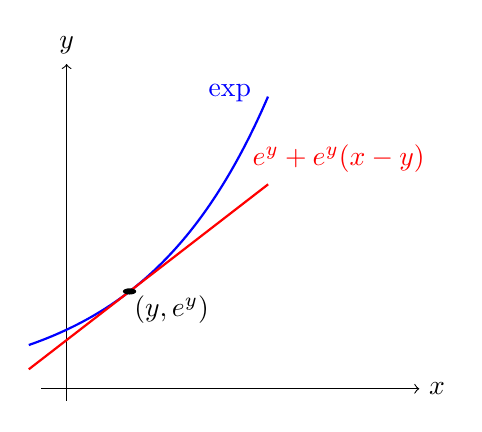
\begin{tikzpicture}[xscale=1.6,yscale=0.75]
\draw[->] (-0.2,0) -- (2.8,0) node[right] {$x$};
\draw[->] (0,-0.2) -- (0,5.5) node[above] {$y$};
\draw[blue,thick,domain=-0.3:1.6,samples=100,smooth] plot (\x,{exp(\x)});
\draw[red,thick,domain=-0.3:1.6,samples=2] plot (\x,{exp(0.5)*(1+\x-0.5)});
\fill (0.5,{exp(0.5)}) circle (1.5pt);
\node[below right, inner sep=1.5pt] at (0.5,{exp(0.5)}) {$(y,e^y)$};
\node[blue,anchor=west] at (1.05,5.0) {$\exp$};
\node[red,anchor=south west] at (1.4,3.5) {$e^y+e^y(x-y)$};
\end{tikzpicture}
\caption{Supporting line: the tangent to $\exp $ at $(y,e^{y})$ lies below
the graph.}
\label{fig:supporting-line}
\end{figure}

\section{Further proofs}

\label{sec:further}

\subsection{Limit definition and Bernoulli's inequality (Seventh proof)}

\begin{theorem}[Convexity via the limit definition and Bernoulli's inequality%
]
\label{thm:bernoulli} $\exp$ is convex on $\R$.
\end{theorem}

\begin{proof}
\noindent\underline{{\large \emph{Step 1: limit definition of $\exp$.}}}

\noindent The exponential is the limit of the sequence $\bigl((1+x/n)^{n}%
\bigr)_{n}$, in the $\varepsilon$-$N$ sense

\begin{ineq}
\label{eq:bern-approx} \forall x\in\R,\ \forall\varepsilon\in\R_{>0},\
\exists N\in\N,\ \forall n\in\N:\quad n\geq N\ \Longrightarrow\ \Bigl|\Bigl(%
1+\frac{x}{n}\Bigr)^{n}-\exp(x)\Bigr|<\varepsilon .
\end{ineq}

\noindent\underline{{\large \emph{Step 2: the inequality $e^{x}\geq 1+x$.}}}

\noindent Fix $x\in \R_{\geq -1}$ and $\varepsilon >0$, and let $N$ be as in %
\cref{eq:bern-approx}. By Bernoulli's inequality, 
\begin{equation*}
\forall n\in \N_{\geq 1}:\quad \Bigl(1+\frac{x}{n}\Bigr)^{n}\geq 1+x.
\end{equation*}%
For every $n\geq N$, therefore, 
\begin{equation*}
\exp (x)>\Bigl(1+\frac{x}{n}\Bigr)^{n}-\varepsilon \geq 1+x-\varepsilon .
\end{equation*}%
Since $\varepsilon >0$ is arbitrary, 
\begin{equation*}
e^{x}\geq 1+x.
\end{equation*}
If $x<-1$, then $1+x<0<e^{x}$, so the inequality holds there too.

Hence

\begin{ineq}
\label{eq:bern-ez} \forall x\in\R:\quad e^{x}\geq 1+x .
\end{ineq}

\noindent\underline{{\large \emph{Step 3: supporting-line criterion.}}}

\noindent Substituting $z=x-y$ in \cref{eq:bern-ez} and multiplying by $%
e^{y}>0$ gives the supporting-line inequality 
\begin{equation*}
\forall x,y\in \R:\quad e^{x}\geq e^{y}+e^{y}(x-y).
\end{equation*}%
By the supporting-line criterion (a differentiable $f$ is convex if and only
if its graph lies above each tangent line; see the proof of %
\Cref{thm:supporting-line}), $\exp $ is convex on $\R$.

\noindent The approximation 
\begin{equation*}
(1+x/n)^{n}\rightarrow e^{x}
\end{equation*}%
is illustrated in Figure~\ref{fig:bernoulli}.
\end{proof}

\begin{figure}[tbph]
\centering
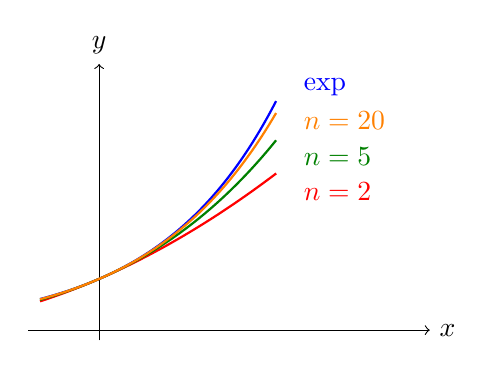
\begin{tikzpicture}[xscale=1.5,yscale=0.65]
\draw[->] (-0.6,0) -- (2.8,0) node[right] {$x$};
\draw[->] (0,-0.2) -- (0,5.2) node[above] {$y$};
\draw[blue,thick,domain=-0.5:1.5,samples=100,smooth] plot (\x,{exp(\x)});
\draw[red,thick,domain=-0.5:1.5,samples=50,smooth]  plot (\x,{(1+\x/2)^2});
\draw[green!50!black,thick,domain=-0.5:1.5,samples=100,smooth] plot (\x,{(1+\x/5)^5});
\draw[orange,thick,domain=-0.5:1.5,samples=150,smooth] plot (\x,{(1+\x/20)^20});
\node[blue,anchor=west]           at (1.65,4.75) {$\exp$};
\node[orange,anchor=west]         at (1.65,4.10) {$n=20$};
\node[green!50!black,anchor=west] at (1.65,3.40) {$n=5$};
\node[red,anchor=west]            at (1.65,2.70) {$n=2$};
\end{tikzpicture}
\caption{Bernoulli's approximation: for each $x\in \R$ and each $\protect%
\varepsilon >0$ there is $N$ such that $\bigl|(1+x/n)^{n}-\exp (x)\bigr|<%
\protect\varepsilon $ for all $n\geq N$.}
\label{fig:bernoulli}
\end{figure}

\subsection{Inverse of the concave logarithm (Eighth proof)}

\begin{theorem}
\label{thm:log-inverse} $\exp $ is convex on $\R$ as the inverse of the
concave logarithm.
\end{theorem}

\begin{proof}
\noindent The logarithm 
\begin{equation*}
\log :\R_{>0}\rightarrow \R,
\end{equation*}
\noindent is strictly concave\comma because 
\begin{equation*}
\log ^{\prime \prime }(x)<0.
\end{equation*}
\noindent The inverse of a strictly increasing concave function is convex.
\noindent Since $\exp $ is the inverse of $\log $\comma\ $\exp $ is convex.
\end{proof}

\subsection{Pointer to the Lean's proof (Ninth proof)}

\noindent The Lean's library contains a proof of \texttt{strict\_convex\_on%
\_exp} that is deliberately elementary and avoids the second-derivative test~%
\cite{LeanMathlib}.\newline
The file is on the path to H\"{o}lder and Minkowski\comma so it cannot
invoke the second-derivative test.

The proof uses a slope argument instead.\newline
We refer to \Cref{sec:lean} for the full mathematical adaptation.

\section{The Lean's proof}

\label{sec:lean}

\subsection{Source code.}

\begin{quotation}
\noindent The Lean file \texttt{analysis/convex/specific%
\_functions/basic.lean} (authors: Yury Kudryashov\comma S\'{e}bastien Gou%
\"{e}zel\comma Heather Macbeth. Copyright 2020\comma Apache 2.0) proves 
\begin{equation*}
\mathtt{strict\_convex\_on\_exp}:\mathtt{strict\_convex\_on}\ \R\ \mathtt{%
univ}\ \exp \text{,}
\end{equation*}%
\noindent and derives 
\begin{equation*}
\mathtt{convex\_on\_exp}:\mathtt{convex\_on}\ \R\ \mathtt{univ}\ \exp \text{%
, }
\end{equation*}%
\noindent by \texttt{strict\_convex\_on\_exp.convex\_on}.

\noindent The file header states that \textquotedblleft the proofs in this
file are deliberately elementary\comma\emph{not} by appealing to the sign of
the second derivative,\textquotedblright \ comma because the file sits early
in the import hierarchy.

\noindent The Lean's proof uses two auxiliary facts, which we now state and
prove in ordinary mathematical language. (See \cite{LeanMathlib})
\end{quotation}

\subsection{Auxiliary lemma (strict supporting-line inequality)}

\begin{lemma}[Strict supporting-line inequality]
\label{lem:strict-supporting} For every $t\in\R$ with $t\neq 0$,

\begin{ineq}
\label{eq:strict-supporting} e^{t}\ >\ 1+t.
\end{ineq}
\end{lemma}

\begin{proof}[Proof 1: direct\comma via the power series]
\noindent If $t>0$\comma then 
\begin{equation*}
e^{t}>1+t\quad \text{because for every }N\geq 2,\ \sum_{n=0}^{N}t^{n}/n!>1+t,%
\text{ and the inequality passes to }\exp (t),
\end{equation*}%
\noindent and every term of the sum is strictly positive\comma so 
\begin{equation*}
\forall t\in \R_{>0}:\text{ }e^{t}>1+t.
\end{equation*}%
\noindent

\begin{itemize}
\item If $-1<t<0$\comma write $t=-s$ with $0<s<1$. \noindent

For each $k\geq 0$\comma the pair of consecutive terms 
\begin{equation*}
\frac{s^{2k}}{(2k)!}-\frac{s^{2k+1}}{(2k+1)!}=\frac{s^{2k}}{(2k)!}\left( 1-%
\frac{s}{2k+1}\right)
\end{equation*}%
\noindent is strictly positive because $s<1\leq 2k+1$. \noindent

For every $K\in \N$ the partial sum%
\begin{equation*}
\sum_{k=0}^{K}\bigl(s^{2k}/(2k)!-s^{2k+1}/(2k+1)!\bigr)
\end{equation*}%
exceeds $1-s$ (the $k=0$ term already contributes $1-s$, every other term is
positive), and the inequality passes to $\exp (-s)$.

\item \noindent If $t\leq -1$\comma then 
\begin{equation*}
1+t\leq 0<e^{t},
\end{equation*}%
so the inequality holds trivially.
\end{itemize}
\end{proof}

\begin{proof}[Proof 2: via the logarithm\comma as in Lean]
\noindent The power-series (or integral) definition of $\log $ gives 
\begin{equation*}
\forall x\in \mathbb{R}_{>0}:\text{ }x\neq 1\Rightarrow \log x<x-1.
\end{equation*}%
\noindent Apply this with $x=e^{t}$ for $t\neq 0$; then $x>0$ and $x\neq 1$,
so 
\begin{equation*}
\log (e^{t})<e^{t}-1\comma
\end{equation*}%
i.e. 
\begin{equation*}
\ t<e^{t}-1\comma
\end{equation*}%
i.e. 
\begin{equation*}
1+t<e^{t}.
\end{equation*}
\end{proof}

\medskip

\noindent Both proofs are elementary.

\begin{itemize}
\item Proof~2 mirrors the Lean derivation (where the strict inequality is
obtained from the log inequality).

\item Proof~1 stays within the power-series framework used throughout this
note.
\end{itemize}

\subsection{Auxiliary lemma (slope criterion)}

\begin{lemma}[Slope criterion for strict convexity]
\label{lem:slope-criterion} Let $I\subseteq \R$ be an interval and $%
f:I\rightarrow \R$. \noindent

The following statements are equivalent:

\begin{enumerate}
\item $f$ is strictly convex on $I$.

\item for all $x<y<z$ in $I$\comma

\begin{ineq}
\label{eq:slope-criterion} \frac{f(y)-f(x)}{y-x}<\frac{f(z)-f(y)}{z-y}.
\end{ineq}
\end{enumerate}
\end{lemma}

\begin{proof}
\noindent For $x<y<z$\comma write 
\begin{equation*}
y=tx+(1-t)z
\end{equation*}
with 
\begin{equation*}
t=(z-y)/(z-x)\in (0,1).
\end{equation*}%
\noindent Then 
\begin{equation*}
y-x=(1-t)(z-x),
\end{equation*}%
\noindent and 
\begin{equation*}
z-y=t(z-x).
\end{equation*}%
\noindent Multiplying \cref{eq:slope-criterion} by $(z-x)>0$ and then by $%
t(1-t)>0$, it becomes 
\begin{equation*}
t\bigl(f(y)-f(x)\bigr)<(1-t)\bigl(f(z)-f(y)\bigr),
\end{equation*}%
\noindent which rearranges to 
\begin{equation*}
f(y)<tf(x)+(1-t)f(z)\comma
\end{equation*}%
the strict convexity inequality.
\end{proof}

\subsection{Proof of the $\exp $ convexity (Lean slope argument)}

\begin{theorem}[Strict convexity of $\exp $\comma Lean form]
\label{thm:exp-strict-convex-lean} \noindent $\exp $ is strictly convex on $%
\R$ by the slope criterion. \noindent Consequently\comma\ $\exp $ is convex
on $\R$.
\end{theorem}

\begin{proof}
\noindent By \Cref{lem:slope-criterion}\comma it suffices to show that for
all $x<y<z$ in $\R$\comma
\begin{equation*}
\frac{e^{y}-e^{x}}{y-x}<\frac{e^{z}-e^{y}}{z-y}.
\end{equation*}
\noindent We prove the stronger chain

\begin{ineq}
\label{eq:slope-chain} \forall x,y,z\in\R:\quad x<y<z\implies \frac{e^y-e^x}{%
y-x}<e^y<\frac{e^z-e^y}{z-y}.
\end{ineq}

\noindent \underline{{\large {\emph{\ Left inequality:}}}} \noindent Put 
\begin{equation*}
h:=y-x>0.
\end{equation*}
By multiplicativity\comma 
\begin{equation*}
e^{y}-e^{x}=e^{y}\bigl(1-e^{x-y}\bigr)=e^{y}\bigl(1-e^{-h}\bigr).
\end{equation*}%
\noindent By \Cref{lem:strict-supporting} with $t=-h\neq 0$\comma we have%
\begin{equation*}
e^{-h}>1-h\comma
\end{equation*}%
so 
\begin{equation*}
1-e^{-h}<h.
\end{equation*}

Hence 
\begin{equation*}
e^{y}-e^{x}<e^{y}\cdot h=e^{y}(y-x).
\end{equation*}%
\noindent Dividing by $y-x>0$ gives 
\begin{equation*}
(e^{y}-e^{x})/(y-x)<e^{y}.
\end{equation*}%
\noindent \underline{{\large {\emph{\ Right inequality:}}}} \noindent Put 
\begin{equation*}
k:=z-y>0.
\end{equation*}
\noindent By multiplicativity\comma 
\begin{equation*}
e^{z}-e^{y}=e^{y}\bigl(e^{z-y}-1\bigr)=e^{y}\bigl(e^{k}-1\bigr).
\end{equation*}%
\noindent By \Cref{lem:strict-supporting} with $t=k\neq 0$\comma we have 
\begin{equation*}
e^{k}>1+k\comma
\end{equation*}%
so 
\begin{equation*}
e^{k}-1>k.
\end{equation*}

\noindent Hence 
\begin{equation*}
e^{z}-e^{y}>e^{y}\cdot k=e^{y}(z-y).
\end{equation*}%
\noindent Dividing by $z-y>0$ gives 
\begin{equation*}
e^{y}<(e^{z}-e^{y})/(z-y).
\end{equation*}%
\noindent Combining\comma\ \cref{eq:slope-chain} holds, so the slopes of $%
\exp $ are strictly increasing.

\noindent By \Cref{lem:slope-criterion}\comma\ $\exp $ is strictly convex on 
$\R$\comma and strict convexity implies convexity.\newline
The chain of slopes in \cref{eq:slope-chain} is drawn in %
\Cref{fig:slope-criterion}.
\end{proof}

\begin{figure}[tbph]
\centering
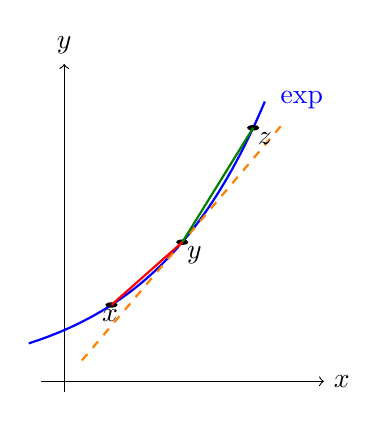
\begin{tikzpicture}[xscale=1.5,yscale=0.65]
	\draw[->] (-0.2,0) -- (2.2,0) node[right] {$x$};
	\draw[->] (0,-0.2) -- (0,6.2) node[above] {$y$};
	\draw[blue,thick,domain=-0.3:1.7,samples=100,smooth] plot (\x,{exp(\x)});
	\draw[orange,dashed,thick,domain=0.15:1.85,samples=2] plot (\x,{exp(1.0)*(1+\x-1.0)});
	\fill (0.4,{exp(0.4)}) circle (1.5pt) node[below left, xshift=4pt, inner sep=1.5pt] {$x$};
	\fill (1.0,{exp(1.0)}) circle (1.5pt) node[below right, inner sep=1.5pt] {$y$};
	\fill (1.6,{exp(1.6)}) circle (1.5pt) node[below right, inner sep=1.5pt] {$z$};
	\draw[red,thick] (0.4,{exp(0.4)}) -- (1.0,{exp(1.0)});
	\draw[green!50!black,thick] (1.0,{exp(1.0)}) -- (1.6,{exp(1.6)});
	\node[blue,anchor=west] at (1.75,5.5) {$\exp$};
	\end{tikzpicture}
\caption{Slope criterion for the Lean proof: for $x<y<z$, the chord from $x$
to $y$ (red) has slope strictly less than the tangent at $y$ (orange, slope $%
e^{y}$), which in turn is strictly less than the slope of the chord from $y$
to $z$ (green).}
\label{fig:slope-criterion}
\end{figure}

\begin{remark}[Relation to \Cref{thm:supporting-line}]
\Cref{thm:supporting-line,thm:exp-strict-convex-lean} both rest on the
supporting-line inequality. \noindent

The structural difference is that \Cref{thm:supporting-line} uses the \emph{%
supporting-line (tangent) criterion} (a differentiable $f$ is convex iff its
graph lies above each tangent line)\comma which requires differentiability,
whereas \Cref{thm:exp-strict-convex-lean} uses the \emph{slope criterion} (a
function is strictly convex iff adjacent slopes are strictly increasing)%
\comma which requires no differentiability and directly yields strict
convexity.\newline
The Lean's proof is in this sense more elementary than %
\Cref{thm:supporting-line}.\newline
The price is the strict auxiliary inequality for $t\neq 0$ 
\begin{equation*}
e^{t}>1+t
\end{equation*}%
rather than the non-strict $e^{t}\geq 1+t$.
\end{remark}

\begin{remark}[The remaining Lean content]
The same Lean file also proves\comma by the same elementary slope and
algebraic methods\comma that:

\begin{itemize}
\item $x\mapsto x^{n}$ is convex on $\R_{>0}$ for every $n\in \N$, and on
all of $\R$ when $n$ is even.

\item $x\mapsto x^{m}$ is convex on $\R_{>0}$ for every $m\in \Z$.

\item $\log $ is strictly concave on $\R_{>0}$ and on $\R_{<0}$.

\item $x\mapsto x^{p}$ is convex on $\R_{>0}$ for $p\geq 1$, and strictly
convex for $p>1$.
\end{itemize}

\noindent These are not needed for the convexity of $\exp $\comma but they
share the same design argument: \textquotedblleft Elementary slope and
algebraic arguments with no second-derivative test.\textquotedblright
\end{remark}

\section{Reverse-mathematical classification proofs}

\label{sec:summary}

{\ \setstretch{1.3} }

\begin{quotation}
\noindent Of the ten routes:\thinspace
\end{quotation}

\begin{itemize}
\item Three are constructive in Bishop's sense (proofs 1,\thinspace
\allowbreak 2,\thinspace \allowbreak 3).

\item \allowbreak Three are classical differential proofs (proofs
4,\thinspace \allowbreak 5,\thinspace \allowbreak 6).

\item \thinspace \allowbreak Two are further classical or analytic proofs
(proofs 7,\thinspace \allowbreak 8).

\item Two concern the formal Lean's proof (proofs 9,\thinspace \allowbreak
10).
\end{itemize}

\begin{quotation}
\noindent The constructive routes share the property that no appeal is made
to the law of excluded middle,\thinspace \allowbreak the mean value
theorem,\thinspace \allowbreak or the second-derivative test.

\noindent The classical routes are standard textbook proofs. \noindent

The formal routes exhibit the same underlying arguments in the language of
the Lean theorem prover,\thinspace \allowbreak with the slope criterion
replacing the supporting-line criterion of the classical proof.
\end{quotation}

\begin{center}
{\small \ 
\begin{tabular}{|m{0.8cm}|m{6.5cm}|m{2.3cm}|m{1.5cm}|}
\hline
\textbf{\#} & \textbf{Mechanism} & \textbf{Reference} & \textbf{Constr.} \\ 
\hline
1 & Weighted AM--GM inequality & \Cref{thm:amgm} & Yes \\ \hline
2 & Direct series on the non-negative reals,\thinspace \allowbreak then
translation & \Cref{thm:series-pos,thm:translation} & Yes \\ \hline
3 & Midpoint convexity via an algebraic square & \Cref{thm:midpoint-convex}
& Yes \\ \hline
4 & Second-derivative test & \Cref{thm:second-derivative} & No \\ \hline
5 & Derivative strictly increasing & \Cref{thm:derivative-increasing} & No
\\ \hline
6 & Supporting line via the series & \Cref{thm:supporting-line} & No \\ 
\hline
7 & Limit definition and Bernoulli & \Cref{thm:bernoulli} & No \\ \hline
8 & Inverse of the concave logarithm & \Cref{thm:log-inverse} & No \\ \hline
9 & Lean's formal proof (pointer) & \S \ref{sec:further} & Formal \\ \hline
10 & Lean's slope proof (detailed) & \Cref{thm:exp-strict-convex-lean} & 
Formal \\ \hline
\end{tabular}
}
\end{center}

\begin{quotation}
{\setstretch{1.2} \noindent The three constructive proofs are independent in
their analytic inputs: \medskip }
\end{quotation}

\begin{itemize}
\item Proof 1 uses the weighted AM--GM inequality.

\item Proof 2 uses monomial convexity on $\R_{+}$.

\item Proof 3 uses the algebraic identity $(\mathtt{Real.exp}\ (x/2)-\mathtt{%
\ Real.exp}\ (y/2))^{2}\geq 0.$
\end{itemize}

\begin{quotation}
\medskip

They share only the power-series definition and its standard consequences.
The two Lean's proofs share the slope criterion and the strict
supporting-line inequality.

Proof 10 in addition uses the multiplicativity of the exponential. \noindent
Sections \ref{sec:constructive}--\ref{sec:lean} prove the convexity of $%
\mathtt{Real.exp}$ via ten independent routes. \noindent

This section re-classifies each route in second-order arithmetic.

Entries carry a strength in $\{\mathsf{FOL},\,\mathsf{RCA}_{0},\,\mathsf{WKL}
_{0},\,\mathsf{ACA}_{0},\,\mathsf{ZF},\,\mathsf{ZFC}\}.$

No route uses $\mathsf{DC}\left( \mathbb{R}\right) $ or any choice principle.
\end{quotation}

\begin{center}
$%
\begin{array}{|c|r|l|}
\hline
\refstepcounter{axctr}\hypertarget{ax:rca}{\mbox{\textbf{Ax\,\theaxctr}}}%
\label{axi:rca} & 
\begin{array}{r}
\text{\textsf{Recursive}} \\ 
\text{\textsf{Comprehension}} \\ 
\text{\textsf{Axiom}}%
\end{array}
& 
\begin{array}{l}
\mathsf{RCA}_{\mathsf{0}}\;=\;\mathsf{FOL}+\Delta _{1}^{0}\text{-CA}+\Sigma
_{1}^{0}\text{-Ind} \\[2pt] 
\text{$\Delta _{1}^{0}$-CA:}\ \ \exists X\,\forall n\,\bigl(n\in X\iff
\varphi (n)\bigr),\quad \varphi \in \Delta _{1}^{0} \\[2pt] 
\text{$\Sigma _{1}^{0}$-Ind:}\ \ \bigl(\varphi (0)\wedge \forall n\,(\varphi
(n)\rightarrow \varphi (n+1))\bigr)\rightarrow \ \forall n\,\varphi
(n),\quad \varphi \in \Sigma _{1}^{0}%
\end{array}
\\ \hline
\refstepcounter{axctr}\hypertarget{ax:wkl}{\mbox{\textbf{Ax\,\theaxctr}}}%
\label{axi:wkl} & 
\begin{array}{r}
\text{\textsf{Weak K\"{o}nig}}\mathsf{^{\prime }}\text{\textsf{s }} \\ 
\text{\textsf{Lemma}}%
\end{array}
& 
\begin{array}{l}
\mathsf{WKL}_{\mathsf{0}}\;=\;\mathsf{RCA}_{\mathsf{0}}+\mathsf{WKL} \\[2pt] 
\mathsf{WKL:}\ \ \forall T\subseteq \{0,1\}^{<\N}\,, \\ 
\Bigl(\forall n\,\exists \sigma \in T\,\bigl(|\sigma |\geq n\bigr)%
\rightarrow \exists f:\N\rightarrow \{0,1\}\,\forall n\,\bigl(%
f\!\upharpoonright \!n\in T\bigr)\Bigr)%
\end{array}%
\end{array}%
$ \noindent $%
\begin{array}{|c|r|l|}
\hline
\refstepcounter{axctr}\hypertarget{ax:aca}{\mbox{\textbf{Ax\,\theaxctr}}}%
\label{axi:aca} & 
\begin{array}{r}
\text{\textsf{Arithmetical}} \\ 
\text{\textsf{Comprehension}} \\ 
\text{\textsf{Axiom}}%
\end{array}
& 
\begin{array}{l}
\mathsf{ACA}_{\mathsf{0}}\;=\;\mathsf{RCA}_{\mathsf{0}}+\text{Arithmetical CA%
} \\[2pt] 
\text{Arithmetical CA:}\ \ \exists X\,\forall n\,\bigl(n\in X\iff \varphi (n)%
\bigr),\text{ }\varphi \text{ Arithmetical}%
\end{array}
\\ \hline
\refstepcounter{axctr}\hypertarget{ax:dc}{\mbox{\textbf{Ax\,\theaxctr}}}%
\label{axi:dc} & 
\begin{array}{r}
\text{\textsf{Dependent Choice}} \\ 
\text{\textsf{on the reals}}%
\end{array}
& 
\begin{array}{l}
\mathsf{ZF+DC}(\mathbb{R})\mathsf{:}\ \ \forall A\subseteq \mathbb{R},\
A\neq \emptyset ,\ \forall R\subseteq A\times A \\ 
\qquad \Bigl(\forall x\in A\,\exists y\in A\,(x\,R\,y)\ \rightarrow \\ 
\qquad \qquad \forall a\in A\,\exists (a_{n})\,\bigl(a_{0}=a\wedge \forall
n\,(a_{n}\,R\,a_{n+1})\bigr)\Bigr)%
\end{array}%
\end{array}%
$ \noindent $%
\begin{array}{|c|r|l|}
\hline
\refstepcounter{axctr}\hypertarget{ax:ac}{\mbox{\textbf{Ax\,\theaxctr}}}%
\label{axi:ac} & 
\begin{array}{r}
\text{\textsf{Axiom of}} \\ 
\text{\textsf{Choice}}%
\end{array}
& 
\begin{array}{l}
\mathsf{ZF+AC:}\ \ \forall I\neq \emptyset \ \forall (A_{i})_{i\in I} \\ 
\qquad \Bigl(\forall i\in I\,(A_{i}\neq \emptyset )\ \rightarrow \exists
f:I\rightarrow \bigcup_{i\in I}A_{i}\ \forall i\in I\,\bigl(f(i)\in A_{i}%
\bigr)\Bigr) \\ 
\qquad \text{i.e. }\mathsf{ZFC}=\mathsf{ZF}+\mathsf{AC}%
\end{array}
\\ \hline
\end{array}%
$
\end{center}

\medskip The table below records the abbreviations used in the \emph{axiom
entries} above and throughout \S \ref{sec:summary}.

\begin{center}
$%
\begin{array}{|l|rc|}
\hline
\mathsf{FOL}:=\text{ first-order logic} & \text{quantifiers over individuals}
& 
\end{array}%
$ \noindent $%
\begin{array}{|l|rc|}
\hline
\text{CA}:=\text{ }\exists X\,\forall n\,(n\in X\iff \varphi (n)) & \text{%
comprehension scheme} &  \\ \hline
\text{Ind}:=\varphi (0)\wedge \forall n\,(\varphi (n)\rightarrow \varphi
(n+1))\rightarrow \forall n\,\varphi (n) & \text{induction scheme} & 
\end{array}%
$ \noindent $%
\begin{array}{|l|rc|}
\hline
\Delta _{1}^{0}\text{-CA} & \text{with }\varphi \in \Delta _{1}^{0} &  \\ 
\hline
\Sigma _{1}^{0}\text{-Ind} & \text{with }\varphi \in \Sigma _{1}^{0} & 
\end{array}%
$ \noindent $%
\begin{array}{|l|rc|}
\hline
\text{arithmetical CA} & \text{with }\varphi \text{ arithmetical} &  \\ 
\hline
\mathsf{RCA}_{\mathsf{0}}:=\mathsf{FOL}+\Delta _{1}^{0}\text{-CA}+\Sigma
_{1}^{0}\text{-Ind} & \text{system} & 
\end{array}%
$ \noindent $%
\begin{array}{|l|rc|}
\hline
\mathsf{WKL:=}\text{ }\forall n\,\exists \sigma \in T\,(|\sigma |\geq
n)\rightarrow \exists f\,\forall n\,(f\upharpoonright n\in T) & \text{weak K%
\"{o}nig's lemma} &  \\ \hline
\mathsf{WKL}_{\mathsf{0}}:=\mathsf{RCA}_{\mathsf{0}}+\mathsf{WKL} & \text{%
system} & 
\end{array}%
$ \noindent $%
\begin{array}{|l|rc|}
\hline
\mathsf{ACA}_{\mathsf{0}}:=\mathsf{RCA}_{\mathsf{0}}+\text{arithmetical CA}
& \text{system} &  \\ \hline
\mathsf{DC}\left( \mathbb{R}\right) \mathsf{:}\text{ \text{\hyperlink{ax:dc}{%
ax:dc}}} & \text{dependent choice on }\mathbb{R} & 
\end{array}%
$ \noindent $%
\begin{array}{|l|rc|}
\hline
\mathsf{AC}\text{\textsf{:} \ \text{\hyperref[axi:ac]{axi:ac}}} & \text{%
axiom of choice} &  \\ \hline
\mathsf{ZF}\text{\textsf{: }Zermelo--Fraenkel} & \text{set theory with }\in
& 
\end{array}%
$ \noindent $%
\begin{array}{|l|rc|}
\hline
\mathsf{ZFC:=ZF}+\mathsf{AC} & \text{with choice} &  \\ \hline
\N:=\{0,1,2,\dots \} & \text{natural numbers} & 
\end{array}%
$ \noindent $%
\begin{array}{|l|rc|}
\hline
f\upharpoonright n:=(f(0),\dots ,f(n-1)) & \text{restriction of }f\text{ to }%
n &  \\ \hline
\{0,1\}^{<\N}:=\bigcup_{n\in \N}\{0,1\}^{n} & \text{finite binary strings} & 
\\ \hline
\end{array}%
$
\end{center}

\subsection{Coding conventions}

\label{sec:convexity-coding}

\begin{quotation}
\noindent We adopt Bishop's \emph{Cauchy real with modulus} coding: a real
is a Cauchy sequence of rationals together with an explicit modulus of
convergence.

Algebraic operations are primitive recursive in the codes.

\noindent A function%
\begin{equation*}
f:I\rightarrow \R
\end{equation*}%
is coded by its graph plus a modulus of uniform continuity on each compact
subinterval.

\noindent We write $\mathcal{N}(x)$ for the Lean neighbourhood filter, i.e.\ 
$\mathcal{N}(x)$ abbreviates \texttt{nhds x}. \noindent In Lean's notation
the power series is 
\begin{equation*}
\forall x:\mathbb{R},\ \mathtt{Real.exp}\ x=L\ \Longleftrightarrow \ \forall
\varepsilon >0,\ \exists N,\ \forall m\geq N:\ \Bigl|L-\sum_{n=0}^{m}x^{n}/(%
\mathsf{Nat.factorial}\ n:\mathbb{R})\Bigr|<\varepsilon .
\end{equation*}%
This is available in $\mathsf{RCA}_{0}$ because the partial sums form a
Cauchy sequence with modulus dominated by $2^{n}/n!$ on $|x|\leq n$.

Multiplicativity: 
\begin{equation*}
\forall x\,y:\mathbb{R},\ \mathtt{Real.exp}\ (x+y)=\mathtt{Real.exp}\ x\cdot 
\mathtt{Real.exp}\ y
\end{equation*}%
follows from the binomial theorem plus $\Sigma _{1}^{0}$-comprehension.
\noindent \emph{Convexity} on $I$ is the second-order formula 
\begin{equation*}
\begin{aligned} \mathsf{Conv}(f, I):\iff {} & \forall x \in I,\ \forall y
\in I,\  \forall t : \mathbb{R},\ 0 \le t \to t \le 1 \to {}\\ & f\bigl(t
\cdot x + (1 - t) \cdot y\bigr) \le t \cdot f(x) + (1 - t) \cdot f(y).
\end{aligned}
\end{equation*}
\end{quotation}

\subsection{Field and order axioms}

\label{sec:convexity-axioms}

\begin{quotation}
\noindent The ordered-field and completeness axioms of $\R$, are in Lean's
notation. \noindent\ All are $\mathsf{ZF}$-realizable. None uses choice.
Under the Bishop--Cauchy coding they are theorems of $\mathsf{RCA}_{0}$.
\medskip
\end{quotation}

\begin{center}
$%
\begin{array}{|c|l|r|c|}
\hline
\refstepcounter{axctr}\hypertarget{ax:conv-add-assoc}{\mbox{\textbf{Ax\,%
\theaxctr}}}\label{axi:conv-add-assoc} & \forall x\,y\,z:\mathbb{R},\
(x+y)+z=x+(y+z) & \mathsf{Add.Assoc.} & \mathsf{ZF} \\ \hline
\refstepcounter{axctr}\hypertarget{ax:conv-add-comm}{\mbox{\textbf{Ax\,%
\theaxctr}}}\label{axi:conv-add-comm} & \forall x\,y:\mathbb{R},\ x+y=y+x & 
\mathsf{Add.Comm.} & \mathsf{ZF}%
\end{array}%
$ \noindent $%
\begin{array}{|c|l|r|c|}
\hline
\refstepcounter{axctr}\hypertarget{ax:conv-add-zero}{\mbox{\textbf{Ax\,%
\theaxctr}}}\label{axi:conv-add-zero} & \forall x:\mathbb{R},\ 0+x=x & 
\mathsf{Add.Id.} & \mathsf{ZF} \\ \hline
\refstepcounter{axctr}\hypertarget{ax:conv-add-inv}{\mbox{\textbf{Ax\,%
\theaxctr}}}\label{axi:conv-add-inv} & \forall x:\mathbb{R},\ x+(-x)=0 & 
\mathsf{Add.Inv.} & \mathsf{ZF}%
\end{array}%
$ \noindent $%
\begin{array}{|c|l|r|c|}
\hline
\refstepcounter{axctr}\hypertarget{ax:conv-mul-assoc}{\mbox{\textbf{Ax\,%
\theaxctr}}}\label{axi:conv-mul-assoc} & \forall x\,y\,z:\mathbb{R},\
(x\cdot y)\cdot z=x\cdot (y\cdot z) & \mathsf{Mul.Assoc.} & \mathsf{ZF} \\ 
\hline
\refstepcounter{axctr}\hypertarget{ax:conv-mul-comm}{\mbox{\textbf{Ax\,%
\theaxctr}}}\label{axi:conv-mul-comm} & \forall x\,y:\mathbb{R},\ x\cdot
y=y\cdot x & \mathsf{Mul.Comm.} & \mathsf{ZF}%
\end{array}%
$ \noindent $%
\begin{array}{|c|l|r|c|}
\hline
\refstepcounter{axctr}\hypertarget{ax:conv-mul-one}{\mbox{\textbf{Ax\,%
\theaxctr}}}\label{axi:conv-mul-one} & \forall x:\mathbb{R},\ 1\cdot x=x & 
\mathsf{Mul.Id.} & \mathsf{ZF} \\ \hline
\refstepcounter{axctr}\hypertarget{ax:conv-mul-inv}{\mbox{\textbf{Ax\,%
\theaxctr}}}\label{axi:conv-mul-inv} & \forall x:\mathbb{R},\ x\neq
0\rightarrow x\cdot x^{-1}=1 & \mathsf{Mul.Inv.} & \mathsf{ZF}%
\end{array}%
$ \noindent $%
\begin{array}{|c|l|r|c|}
\hline
\refstepcounter{axctr}\hypertarget{ax:conv-distrib}{\mbox{\textbf{Ax\,%
\theaxctr}}}\label{axi:conv-distrib} & \forall x\,y\,z:\mathbb{R},\ x\cdot
(y+z)=x\cdot y+x\cdot z & \mathsf{Distrib.} & \mathsf{ZF} \\ \hline
\refstepcounter{axctr}\hypertarget{ax:conv-nontriv}{\mbox{\textbf{Ax\,%
\theaxctr}}}\label{axi:conv-nontriv} & (0:\mathbb{R})\neq 1 & \mathsf{%
Nontriv.} & \mathsf{ZF}%
\end{array}%
$ \noindent $%
\begin{array}{|c|l|r|c|}
\hline
\refstepcounter{axctr}\hypertarget{ax:conv-order}{\mbox{\textbf{Ax\,%
\theaxctr}}}\label{axi:conv-order} & 
\begin{array}{l}
\bigl(\forall x:\mathbb{R},\ x\leq x\bigr) \\ 
\wedge \bigl(\forall x\,y:\mathbb{R},\ x\leq y\rightarrow y\leq x\rightarrow
x=y\bigr) \\ 
\wedge \bigl(\forall x\,y\,z:\mathbb{R},\ x\leq y\rightarrow y\leq
z\rightarrow x\leq z\bigr) \\ 
\wedge \bigl(\forall x\,y:\mathbb{R},\ x\leq y\vee y\leq x\bigr)%
\end{array}
& \mathsf{LinOrder} & \mathsf{ZF} \\ \hline
\refstepcounter{axctr}\hypertarget{ax:conv-add-mon}{\mbox{\textbf{Ax\,%
\theaxctr}}}\label{axi:conv-add-mon} & \forall x\,y\,z:\mathbb{R},\ x\leq
y\rightarrow x+z\leq y+z & \mathsf{AddMon} & \mathsf{ZF}%
\end{array}%
$ \noindent $%
\begin{array}{|c|l|r|c|}
\hline
\refstepcounter{axctr}\hypertarget{ax:conv-mul-mon}{\mbox{\textbf{Ax\,%
\theaxctr}}}\label{axi:conv-mul-mon} & \forall x\,y:\mathbb{R},\ 0\leq
x\rightarrow 0\leq y\rightarrow 0\leq x\cdot y & \mathsf{MulMon} & \mathsf{ZF%
} \\ \hline
\refstepcounter{axctr}\hypertarget{ax:conv-complete}{\mbox{\textbf{Ax\,%
\theaxctr}}}\label{axi:conv-complete} & 
\begin{array}{l}
\forall S:\mathsf{Set}\ \mathbb{R},\ \bigl(\exists x,\ x\in S\bigr)%
\rightarrow {} \\ 
\quad \bigl(\exists M,\ \forall x\in S,\ x\leq M\bigr)\rightarrow {} \\ 
\quad \exists s,\ \mathsf{IsLUB}\ S\ s%
\end{array}
& \mathsf{Cut} & \mathsf{ZF} \\ \hline
\end{array}%
$
\end{center}

\begin{quotation}
\medskip \noindent The Cut axiom enters no convexity proof in this section:
\noindent The series for \texttt{Real.exp} converges with an explicit
modulus, so no completeness is needed. \noindent All ten routes are
therefore \emph{Cut-free}.
\end{quotation}

\subsection{Postulates}

\label{sec:convexity-postulates}

\begin{quotation}
\noindent Internal statements, each tagged with its strength over $\mathsf{%
RCA}_{0}$, in Lean's notation.
\end{quotation}

\begin{itemize}
\item $(\,\cdot :\mathbb{R})$ denotes the coercion $\mathbb{Q}\rightarrow 
\mathbb{R}$.

\item Routes 1, 2, 3, 6, 7, 8, 9, and 10 use only $\mathsf{RCA}_{0}$ entries.

\item Routes 4 and 5 invoke the general second-derivative test and the
monotone-derivative criterion.
\end{itemize}

\begin{quotation}
Those, together with the two FTC tools they depend on (\textsf{conv-FTC} and 
\textsf{conv-int-strict}), are $\mathsf{WKL}_{0}$ over $\mathsf{RCA}_{0}$
(see~\cite[II.7, IV.2.3]{Simpson2009}), so Routes 4 and 5 are classified as $%
\mathsf{WKL}_{0}$. The classical mean value theorem (\textsf{MVT}) is
recorded as a classical reference only and is not used directly by any route.

\noindent The postulate \textsf{ExpPow} is stated for real $t$. Its $\mathsf{%
RCA}_{0}$-derivation parallels the rational-to-real passage used in %
\Cref{lem:weighted-amgm}: the rational case 
\begin{equation*}
\exp ((m/n)x)=(\exp x)^{m/n}
\end{equation*}
follows from multiplicativity (\textsf{ExpMult}) and the existence of $n$-th
roots, and the passage to real $t$ is by continuity of 
\begin{eqnarray*}
t &\mapsto &\exp (tx) \\
t &\mapsto &(\exp x)^{t},
\end{eqnarray*}
both available in $\mathsf{RCA}_{0}$ from the power-series modulus.

It is recorded as a single postulate only for brevity; its status is that of
a derived $\mathsf{RCA}_{0}$-postulate, exactly as 
\begin{equation*}
\mathsf{AMGM}\left( \mathsf{%
%TCIMACRO{\U{211d} }%
%BeginExpansion
\mathbb{R}
%EndExpansion
}\right) \longleftarrow \mathsf{AMGM}\left( 
%TCIMACRO{\U{211a} }%
%BeginExpansion
\mathbb{Q}
%EndExpansion
\right) .\medskip
\end{equation*}
\end{quotation}

\begin{center}
$%
\begin{array}{|c|l|r|c|}
\hline
\refstepcounter{posctr}\hypertarget{pos:conv-arch}{\mbox{\textbf{Pos\,%
\theposctr}}}\label{posi:conv-arch} & \forall x:\mathbb{R},\ \exists M:%
\mathbb{N},\ |x|\leq (M:\mathbb{R}) & \mathsf{Arch} & \mathsf{RCA}_{0} \\ 
\hline
\refstepcounter{posctr}\hypertarget{pos:conv-amgm-rat}{\mbox{\textbf{Pos\,%
\theposctr}}}\label{posi:conv-amgm-rat} & 
\begin{array}{l}
\forall a\,b:\mathbb{R},\ 0<a\rightarrow 0<b\rightarrow {} \\ 
\quad \forall t:\mathbb{Q},\ 0\leq t\rightarrow t\leq 1\rightarrow {} \\ 
\quad \mathtt{Real.rpow}\ a\ (t:\mathbb{R})\cdot \mathtt{Real.rpow}\ b\
(1-(t:\mathbb{R})) \\ 
\quad \quad \leq (t:\mathbb{R})\cdot a+(1-(t:\mathbb{R}))\cdot b%
\end{array}
& \mathsf{AMGM}\left( \mathsf{\mathbb{Q} }\right) & \mathsf{RCA}_{0}%
\end{array}%
$ \noindent $%
\begin{array}{|c|l|r|c|}
\hline
\refstepcounter{posctr}\hypertarget{pos:conv-amgm-real}{\mbox{\textbf{Pos\,%
\theposctr}}}\label{posi:conv-amgm-real} & 
\begin{array}{l}
\forall a\,b:\mathbb{R},\ 0<a\rightarrow 0<b\rightarrow {} \\ 
\quad \forall t:\mathbb{R},\ 0\leq t\rightarrow t\leq 1\rightarrow {} \\ 
\quad \mathtt{Real.rpow}\ a\ t\cdot \mathtt{Real.rpow}\ b\ (1-t)\leq t\cdot
a+(1-t)\cdot b%
\end{array}
& \mathsf{AMGM}\left( \mathbb{R} \right) & \mathsf{RCA}_{0} \\ \hline
\refstepcounter{posctr}\hypertarget{pos:conv-series-cauchy}{%
\mbox{\textbf{Pos\,\theposctr}}}\label{posi:conv-series-cauchy} & 
\begin{array}{l}
\forall x:\mathbb{R},\ \forall \varepsilon :\mathbb{R},\ 0<\varepsilon
\rightarrow {} \\ 
\quad \exists N:\mathbb{N},\ \forall m\,n:\mathbb{N},\ N\leq n\rightarrow
n\leq m\rightarrow {} \\ 
\quad \Bigl|\sum_{k\in \mathsf{Finset.Icc}\,n\,m}x^{k}/(\mathsf{Nat.factorial%
}\ k:\mathbb{R})\Bigr|<\varepsilon%
\end{array}
& \mathsf{SerCauchy} & \mathsf{RCA}_{0}%
\end{array}%
$ \noindent $%
\begin{array}{|c|l|r|c|}
\hline
\refstepcounter{posctr}\hypertarget{pos:conv-exp-mult}{\mbox{\textbf{Pos\,%
\theposctr}}}\label{posi:conv-exp-mult} & \forall x\,y:\mathbb{R},\ \mathtt{%
Real.exp}\ (x+y)=\mathtt{Real.exp}\ x\cdot \mathtt{Real.exp}\ y & \mathsf{%
ExpMult} & \mathsf{RCA}_{0} \\ \hline
\refstepcounter{posctr}\hypertarget{pos:conv-exp-tx}{\mbox{\textbf{Pos\,%
\theposctr}}}\label{posi:conv-exp-tx} & 
\begin{array}{l}
\forall x:\mathbb{R},\ \forall t:\mathbb{R},\ 0\leq t\rightarrow t\leq
1\rightarrow {} \\ 
\quad \mathtt{Real.exp}\ (t\cdot x)=\mathtt{Real.rpow}\ (\mathtt{Real.exp}\
x)\ t%
\end{array}
& \mathsf{ExpPow} & \mathsf{RCA}_{0}%
\end{array}%
$ \noindent $%
\begin{array}{|c|l|r|c|}
\hline
\refstepcounter{posctr}\hypertarget{pos:conv-monomial}{\mbox{\textbf{Pos\,%
\theposctr}}}\label{posi:conv-monomial} & 
\begin{array}{l}
\forall n:\mathbb{N},\ 1\leq n\rightarrow {} \\ 
\quad \forall x\,y:\mathbb{R},\ 0\leq x\rightarrow 0\leq y\rightarrow {} \\ 
\quad \forall t:\mathbb{R},\ 0\leq t\rightarrow t\leq 1\rightarrow {} \\ 
\quad \quad (t\cdot x+(1-t)\cdot y)^{n}\leq t\cdot x^{n}+(1-t)\cdot y^{n}%
\end{array}
& \mathsf{Monom.} & \mathsf{RCA}_{0} \\ \hline
\refstepcounter{posctr}\hypertarget{pos:conv-midpoint}{\mbox{\textbf{Pos\,%
\theposctr}}}\label{posi:conv-midpoint} & \forall x\,y:\mathbb{R},\ \mathtt{%
Real.exp}\ ((x+y)/2)\leq (\mathtt{Real.exp}\ x+\mathtt{Real.exp}\ y)/2 & 
\mathsf{Midpt} & \mathsf{RCA}_{0} \\ 
&  &  & 
\end{array}%
$ \noindent $%
\begin{array}{|c|l|r|c|}
\hline
\refstepcounter{posctr}\hypertarget{pos:conv-midpoint-real}{%
\mbox{\textbf{Pos\,\theposctr}}}\label{posi:conv-midpoint-real} & 
\begin{array}{l}
\forall f:\mathbb{R}\rightarrow \mathbb{R},\ \mathsf{MidpointConvexOn}\ 
\mathbb{R}\ \mathsf{Set.univ}\ f\rightarrow {} \\ 
\quad \mathsf{Continuous}\ f\rightarrow \mathsf{ConvexOn}\ \mathbb{R}\ 
\mathsf{Set.univ}\ f%
\end{array}
& \mathsf{Mid2Conv} & \mathsf{RCA}_{0} \\ \hline
\refstepcounter{posctr}\hypertarget{pos:conv-FTC}{\mbox{\textbf{Pos\,%
\theposctr}}}\label{posi:conv-FTC} & 
\begin{array}{l}
\forall f:\mathbb{R}\rightarrow \mathbb{R},\ \forall a\,b:\mathbb{R},\
a<b\rightarrow {} \\ 
\quad \mathsf{ContinuousOn}\ f\ (\mathsf{Set.Icc}\ a\ b)\rightarrow {} \\ 
\quad \mathsf{DifferentiableOn}\ \mathbb{R}\ f\ (\mathsf{Set.Ioo}\ a\
b)\rightarrow {} \\ 
\quad \mathsf{ContinuousOn}\ (\mathsf{deriv}\ f)\ (\mathsf{Set.Icc}\ a\
b)\rightarrow {} \\ 
\quad \int_{a}^{b}\mathsf{deriv}\ f\ t\,dt=f\,b-f\,a%
\end{array}
& \mathsf{FTC} & \mathsf{WKL}_{0}%
\end{array}%
$ \noindent $%
\begin{array}{|c|l|r|c|}
\hline
\refstepcounter{posctr}\hypertarget{pos:conv-int-strict}{\mbox{\textbf{Pos\,%
\theposctr}}}\label{posi:conv-int-strict} & 
\begin{array}{l}
\forall g\,h:\mathbb{R}\rightarrow \mathbb{R},\ \forall a\,b:\mathbb{R},\
a<b\rightarrow {} \\ 
\quad \mathsf{ContinuousOn}\ g\ (\mathsf{Set.Icc}\ a\ b)\rightarrow {} \\ 
\quad \mathsf{ContinuousOn}\ h\ (\mathsf{Set.Icc}\ a\ b)\rightarrow {} \\ 
\quad \bigl(\forall t\in \mathsf{Set.Ioo}\ a\ b,\ g\,t<h\,t\bigr)\rightarrow
{} \\ 
\quad \int_{a}^{b}g\,t\,dt<\int_{a}^{b}h\,t\,dt%
\end{array}
& \mathsf{IntStr} & \mathsf{WKL}_{0} \\ \hline
\refstepcounter{posctr}\hypertarget{pos:conv-deriv-pos-mono}{%
\mbox{\textbf{Pos\,\theposctr}}}\label{posi:conv-deriv-pos-mono} & 
\begin{array}{l}
\forall f:\mathbb{R}\rightarrow \mathbb{R},\ \mathsf{ContDiff}\ \mathbb{R}\
2\ f\rightarrow {} \\ 
\quad \bigl(\forall x:\mathbb{R},\ \mathsf{deriv}\ (\mathsf{deriv}\ f)\ x>0%
\bigr)\rightarrow {} \\ 
\quad \mathsf{StrictMono}\ (\mathsf{deriv}\ f)%
\end{array}
& \mathsf{DerPosMono} & \mathsf{WKL}_{0}%
\end{array}%
$ \noindent $%
\begin{array}{|c|l|r|c|}
\hline
\refstepcounter{posctr}\hypertarget{pos:conv-MVT}{\mbox{\textbf{Pos\,%
\theposctr}}}\label{posi:conv-MVT} & 
\begin{array}{l}
\forall f:\mathbb{R}\rightarrow \mathbb{R},\ \forall a\,b:\mathbb{R},\
a<b\rightarrow {} \\ 
\quad \mathsf{ContinuousOn}\ f\ (\mathsf{Set.Icc}\ a\ b)\rightarrow {} \\ 
\quad \mathsf{DifferentiableOn}\ \mathbb{R}\ f\ (\mathsf{Set.Ioo}\ a\
b)\rightarrow {} \\ 
\quad \exists c\in \mathsf{Set.Ioo}\ a\ b,\ \mathsf{deriv}\ f\
c=(f\,b-f\,a)/(b-a)%
\end{array}
& \mathsf{MVT} & \mathsf{WKL}_{0} \\ \hline
\refstepcounter{posctr}\hypertarget{pos:conv-deriv-mon}{\mbox{\textbf{Pos\,%
\theposctr}}}\label{posi:conv-deriv-mon} & 
\begin{array}{l}
\forall f:\mathbb{R}\rightarrow \mathbb{R},\ \mathsf{Continuous}\
f\rightarrow \mathsf{Differentiable}\ \mathbb{R}\ f\rightarrow {} \\ 
\quad \mathsf{Monotone}\ (\mathsf{deriv}\ f)\rightarrow \mathsf{ConvexOn}\ 
\mathbb{R}\ \mathsf{Set.univ}\ f%
\end{array}
& \mathsf{DerMon} & \mathsf{WKL}_{0}%
\end{array}%
$ \noindent $%
\begin{array}{|c|l|r|c|}
\hline
\refstepcounter{posctr}\hypertarget{pos:conv-support}{\mbox{\textbf{Pos\,%
\theposctr}}}\label{posi:conv-support} & 
\begin{array}{l}
\forall f:\mathbb{R}\rightarrow \mathbb{R},\ \bigl(\forall x\,y:\mathbb{R},\
f\,x\geq f\,y+\mathsf{deriv}\ f\,y\cdot (x-y)\bigr)\rightarrow {} \\ 
\quad \mathsf{ConvexOn}\ \mathbb{R}\ \mathsf{Set.univ}\ f%
\end{array}
& \mathsf{Support} & \mathsf{RCA}_{0} \\ \hline
\refstepcounter{posctr}\hypertarget{pos:conv-ez}{\mbox{\textbf{Pos\,%
\theposctr}}}\label{posi:conv-ez} & \forall z:\mathbb{R},\ \mathtt{Real.exp}%
\ z\geq 1+z & \mathsf{EZ} & \mathsf{RCA}_{0}%
\end{array}%
$ \noindent $%
\begin{array}{|c|l|r|c|}
\hline
\refstepcounter{posctr}\hypertarget{pos:conv-bernoulli}{\mbox{\textbf{Pos\,%
\theposctr}}}\label{posi:conv-bernoulli} & 
\begin{array}{l}
\forall x:\mathbb{R},\ -1\leq x\rightarrow {} \\ 
\quad \forall n:\mathbb{N},\ 1\leq n\rightarrow (1+x/(n:\mathbb{R}))^{n}\geq
1+x%
\end{array}
& \mathsf{Bern} & \mathsf{RCA}_{0} \\ \hline
\refstepcounter{posctr}\hypertarget{pos:conv-log-concave}{%
\mbox{\textbf{Pos\,\theposctr}}}\label{posi:conv-log-concave} & \mathsf{%
StrictConcaveOn}\ \mathbb{R}\ (\mathsf{Set.Ioi}\ 0)\ \mathtt{Real.log} & 
\mathsf{LogConc} & \mathsf{RCA}_{0}%
\end{array}%
$ \noindent $%
\begin{array}{|c|l|r|c|}
\hline
\refstepcounter{posctr}\hypertarget{pos:conv-log-inv}{\mbox{\textbf{Pos\,%
\theposctr}}}\label{posi:conv-log-inv} & 
\begin{array}{l}
\forall f\,g:\mathbb{R}\rightarrow \mathbb{R},\ \mathsf{Set.InvOn}\ g\ f\ (%
\mathsf{Set.Ioi}\ 0)\ (f\mathbin{''}\mathsf{Set.Ioi}\ 0)\rightarrow {} \\ 
\quad \mathsf{StrictMonoOn}\ f\ (\mathsf{Set.Ioi}\ 0)\rightarrow {} \\ 
\quad \mathsf{StrictConcaveOn}\ \mathbb{R}\ (\mathsf{Set.Ioi}\ 0)\
f\rightarrow {} \\ 
\quad \mathsf{StrictConvexOn}\ \mathbb{R}\ (f\mathbin{''}\mathsf{Set.Ioi}\
0)\ g%
\end{array}
& \mathsf{LogInv} & \mathsf{RCA}_{0} \\ \hline
\refstepcounter{posctr}\hypertarget{pos:conv-strict-support}{%
\mbox{\textbf{Pos\,\theposctr}}}\label{posi:conv-strict-support} & \forall t:%
\mathbb{R},\ t\neq 0\rightarrow \mathtt{Real.exp}\ t>1+t & \mathsf{StrSupp}
& \mathsf{RCA}_{0}%
\end{array}%
$ \noindent $%
\begin{array}{|c|l|r|c|}
\hline
\refstepcounter{posctr}\hypertarget{pos:conv-slope-crit}{\mbox{\textbf{Pos\,%
\theposctr}}}\label{posi:conv-slope-crit} & 
\begin{array}{l}
\forall f:\mathbb{R}\rightarrow \mathbb{R},\ \mathsf{StrictConvexOn}\ 
\mathbb{R}\ \mathsf{Set.univ}\ f\leftrightarrow {} \\ 
\quad \forall x\,y\,z:\mathbb{R},\ x<y\rightarrow y<z\rightarrow {} \\ 
\quad (f\,y-f\,x)/(y-x)<(f\,z-f\,y)/(z-y)%
\end{array}
& \mathsf{SlopeCrit} & \mathsf{RCA}_{0} \\ \hline
\refstepcounter{posctr}\hypertarget{pos:conv-seq-cont}{\mbox{\textbf{Pos\,%
\theposctr}}}\label{posi:conv-seq-cont} & 
\begin{array}{l}
\forall f:\mathbb{R}\rightarrow \mathbb{R},\ \forall x:\mathbb{R},\ \forall
u:\mathbb{N}\rightarrow \mathbb{R},\ \mathsf{ContinuousAt}\ f\ x\rightarrow
{} \\ 
\quad \mathsf{Filter.Tendsto}\ u\ \mathsf{Filter.atTop}\ (\mathcal{N}\
x)\rightarrow {} \\ 
\quad \mathsf{Filter.Tendsto}\ (\lambda n,\ f\,(u\,n))\ \mathsf{Filter.atTop}%
\ (\mathcal{N}\ (f\,x))%
\end{array}
& \mathsf{SeqCont} & \mathsf{RCA}_{0}%
\end{array}%
$ \noindent $%
\begin{array}{|c|l|r|c|}
\hline
\refstepcounter{posctr}\hypertarget{pos:conv-exp-pos}{\mbox{\textbf{Pos\,%
\theposctr}}}\label{posi:conv-exp-pos} & \forall x:\mathbb{R},\ \mathtt{%
Real.exp}\ x>0 & \mathsf{ExpPos} & \mathsf{RCA}_{0} \\ \hline
\refstepcounter{posctr}\hypertarget{pos:conv-exp-deriv}{\mbox{\textbf{Pos\,%
\theposctr}}}\label{posi:conv-exp-deriv} & \forall x:\mathbb{R},\ \mathsf{%
deriv}\ \mathtt{Real.exp}\ x=\mathtt{Real.exp}\ x & \mathsf{ExpDeriv} & 
\mathsf{RCA}_{0}%
\end{array}%
$ \noindent $%
\begin{array}{|c|l|r|c|}
\hline
\refstepcounter{posctr}\hypertarget{pos:conv-exp-cont}{\mbox{\textbf{Pos\,%
\theposctr}}}\label{posi:conv-exp-cont} & \mathsf{Continuous}\ \mathtt{%
Real.exp} & \mathsf{ExpCont} & \mathsf{RCA}_{0} \\ \hline
\refstepcounter{posctr}\hypertarget{pos:conv-exp-c2}{\mbox{\textbf{Pos\,%
\theposctr}}}\label{posi:conv-exp-c2} & \mathsf{ContDiff}\ \mathbb{R}\ 2\ 
\mathtt{Real.exp} & \mathsf{ExpC2} & \mathsf{RCA}_{0}%
\end{array}%
$ \noindent $%
\begin{array}{|c|l|r|c|}
\hline
\refstepcounter{posctr}\hypertarget{pos:conv-2nd}{\mbox{\textbf{Pos\,%
\theposctr}}}\label{posi:conv-2nd} & 
\begin{array}{l}
\forall f:\mathbb{R}\rightarrow \mathbb{R},\ \mathsf{ContDiff}\ \mathbb{R}\
2\ f\rightarrow {} \\ 
\quad \bigl(\forall x:\mathbb{R},\ \mathsf{deriv}\ (\mathsf{deriv}\ f)\ x>0%
\bigr)\rightarrow {} \\ 
\quad \mathsf{StrictConvexOn}\ \mathbb{R}\ \mathsf{Set.univ}\ f%
\end{array}
& \mathsf{Conv2nd} & \mathsf{WKL}_{0} \\ \hline
\refstepcounter{posctr}\hypertarget{pos:conv-deriv-strict}{%
\mbox{\textbf{Pos\,\theposctr}}}\label{posi:conv-deriv-strict} & 
\begin{array}{l}
\forall f:\mathbb{R}\rightarrow \mathbb{R},\ \mathsf{ContDiff}\ \mathbb{R}\
1\ f\rightarrow {} \\ 
\quad \mathsf{StrictMono}\ (\mathsf{deriv}\ f)\rightarrow \mathsf{%
StrictConvexOn}\ \mathbb{R}\ \mathsf{Set.univ}\ f%
\end{array}
& \mathsf{ConvDerStr} & \mathsf{WKL}_{0}%
\end{array}%
$ \noindent $%
\begin{array}{|c|l|r|c|}
\hline
\refstepcounter{posctr}\hypertarget{pos:conv-limit-exp}{\mbox{\textbf{Pos\,%
\theposctr}}}\label{posi:conv-limit-exp} & 
\begin{array}{l}
\forall x\in \R,\ \forall \varepsilon \in \R_{>0},\ \exists N\in \N,\
\forall n\in \N:\quad n\geq N\Rightarrow \\ 
\quad \Bigl|(1+x/(n:\R))^{n}-\mathtt{Real.exp}\ x\Bigr|<\varepsilon%
\end{array}
& \mathsf{LimitExp} & \mathsf{RCA}_{0} \\ \hline
\refstepcounter{posctr}\hypertarget{pos:conv-exp-log-eq}{\mbox{\textbf{Pos\,%
\theposctr}}}\label{posi:conv-exp-log-eq} & 
\begin{array}{l}
\forall x:\mathbb{R},\ \mathtt{Real.log}\ (\mathtt{Real.exp}\ x)=x\wedge {}
\\ 
\quad \bigl(\forall x:\mathbb{R},\ 0<x\rightarrow \mathtt{Real.exp}\ (%
\mathtt{Real.log}\ x)=x\bigr)%
\end{array}
& \mathsf{ExpLogEq} & \mathsf{RCA}_{0}%
\end{array}%
$ \noindent $%
\begin{array}{|c|l|r|c|}
\hline
\refstepcounter{posctr}\hypertarget{pos:conv-log-mono}{\mbox{\textbf{Pos\,%
\theposctr}}}\label{posi:conv-log-mono} & \mathsf{StrictMonoOn}\ \mathtt{%
Real.log}\ (\mathsf{Set.Ioi}\ 0) & \mathsf{LogMono} & \mathsf{RCA}_{0} \\ 
\hline
\end{array}%
$
\end{center}

\subsection{Definitions}

\label{sec:convexity-definitions}

\begin{quotation}
\noindent Definitional abbreviations available in $\mathsf{RCA}_{0}$:

Set notation by $\Delta _{1}^{0}$-comprehension: $\mathsf{Conv}$, $\mathsf{%
StrictConv}$, $\mathsf{Cont}$ by $\Sigma _{1}^{0}$ predicates. $\mathtt{%
Real.exp}$, $\mathtt{Real.log}$ by unique existence + graphs. \medskip
\end{quotation}

\begin{center}
$%
\begin{array}{|c|l|r|c|}
\hline
\refstepcounter{defctr}\hypertarget{def:conv-exp}{\mbox{\textbf{Def\,			%
\thedefctr}}}\label{defi:conv-exp} & 
\begin{array}{l}
\mathtt{Real.exp}\ x:=L\ \text{(the unique }L\text{ such that)} \\[2pt] 
\qquad\forall\varepsilon\in\mathbb{R}_{>0}\,\exists N\in\mathbb{N}\,\forall
m\geq N:\ \Bigl|L-\sum_{k=0}^{m}x^{k}/k!\Bigr|<\varepsilon%
\end{array}
& \mathsf{exp} & \mathsf{RCA}_{0} \\ \hline
\refstepcounter{defctr}\hypertarget{def:conv-conv}{\mbox{\textbf{Def\,%
\thedefctr}}}\label{defi:conv-conv} & 
\begin{array}{l}
\mathsf{Conv}(f,I):\iff \forall x\in I,\ \forall y\in I,\ \forall t:\mathbb{R%
},\ 0\leq t\rightarrow t\leq 1\rightarrow {} \\ 
\quad f\bigl(t\cdot x+(1-t)\cdot y\bigr)\leq t\cdot f(x)+(1-t)\cdot f(y)%
\end{array}
& \mathsf{Conv} & \mathsf{RCA}_{0}%
\end{array}%
$ \noindent $%
\begin{array}{|c|l|r|c|}
\hline
\refstepcounter{defctr}\hypertarget{def:conv-strict}{\mbox{\textbf{Def\,%
\thedefctr}}}\label{defi:conv-strict} & 
\begin{array}{l}
\mathsf{StrictConv}(f,I):\iff \mathsf{Conv}(f,I)\wedge {} \\ 
\quad \bigl(\forall x\in I,\ \forall y\in I,\ x\neq y\rightarrow {} \\ 
\quad \forall t:\mathbb{R},\ 0<t\rightarrow t<1\rightarrow {} \\ 
\quad \quad f\bigl(t\cdot x+(1-t)\cdot y\bigr)<t\cdot f(x)+(1-t)\cdot f(y)%
\bigr)%
\end{array}
& \mathsf{StrConv} & \mathsf{RCA}_{0} \\ \hline
\refstepcounter{defctr}\hypertarget{def:conv-cont}{\mbox{\textbf{Def\,%
\thedefctr}}}\label{defi:conv-cont} & 
\begin{array}{l}
\mathsf{Cont}(f,I):\iff \forall a\,b:\mathbb{R},\ a<b\rightarrow \forall
\varepsilon :\mathbb{R},\ 0<\varepsilon \rightarrow {} \\ 
\quad \exists \delta :\mathbb{R},\ 0<\delta \wedge {} \\ 
\quad \forall x\in I\cap \mathsf{Set.Icc}\ a\ b,\ \forall y\in I\cap \mathsf{%
Set.Icc}\ a\ b,\ {} \\ 
\quad \quad |x-y|<\delta \rightarrow |f\,x-f\,y|<\varepsilon%
\end{array}
& \mathsf{Cont} & \mathsf{RCA}_{0} \\ 
\end{array}%
$ \noindent $%
\begin{array}{|c|l|r|c|}
\hline
\refstepcounter{defctr}\hypertarget{def:conv-midpoint}{\mbox{\textbf{Def\,%
\thedefctr}}}\label{defi:conv-midpoint} & \mathsf{Midpoint}(f,I):\iff
\forall x\in I,\ \forall y\in I,\ f((x+y)/2)\leq (f\,x+f\,y)/2 & \mathsf{%
Midpt} & \mathsf{RCA}_{0} \\ \hline
\refstepcounter{defctr}\hypertarget{def:conv-slope}{\mbox{\textbf{Def\,%
\thedefctr}}}\label{defi:conv-slope} & \mathsf{Slope}(f,x,y):=(f\,y-f%
\,x)/(y-x)\ \text{for }x\neq y & \mathsf{Slope} & \mathsf{RCA}_{0} \\ 
\end{array}%
$ \noindent $%
\begin{array}{|c|l|r|c|}
\hline
\refstepcounter{defctr}\hypertarget{def:conv-diff}{\mbox{\textbf{Def\,%
\thedefctr}}}\label{defi:conv-diff} & 
\begin{array}{l}
\mathsf{Diff}(f,x):\iff \exists L,\ \mathsf{Filter.Tendsto}\ (\lambda h,\
(f\,(x+h)-f\,x)/h)\ (\mathcal{N}\ 0)\ (\mathcal{N}\ L) \\ 
\text{and then } \mathsf{deriv}\ f\ x:=\text{the unique such }L%
\end{array}
& \mathsf{Diff} & \mathsf{RCA}_{0} \\ \hline
\refstepcounter{defctr}\hypertarget{def:conv-Ck}{\mbox{\textbf{Def\,%
\thedefctr}}}\label{defi:conv-Ck} & C^{k}(I)(f):\iff \exists g_{0},\dots
,g_{k},\ g_{0}=f\wedge \forall j<k,\ g_{j+1}=\mathsf{deriv}\ g_{j} & \mathsf{%
C^{k}} & \mathsf{RCA}_{0}%
\end{array}%
$ \noindent $%
\begin{array}{|c|l|r|c|}
\hline
\refstepcounter{defctr}\hypertarget{def:conv-log}{\mbox{\textbf{Def\,			%
\thedefctr}}}\label{defi:conv-log} & 
\begin{array}{l}
\mathtt{Real.log}\ x:=\text{the unique }y\text{ such that }\mathtt{Real.exp}%
\ y = x\quad(x > 0)\text{;} \\[2pt] 
\text{the identity }\mathtt{Real.log}\ x = \int_1^x dt/t \text{ is a
consequence of the FTC,} \\[2pt] 
\text{hence }\mathsf{WKL}_0\text{-provable, and is \emph{not} used as a
definitional basis.} \\[2pt] 
\text{Existence of }y\text{ from }\mbox{Pos:\ref{posi:conv-arch}}\text{ +
monotone IVT; uniqueness from }\mbox{Pos:\ref{posi:conv-strict-support}}.%
\end{array}
& \mathsf{log} & \mathsf{RCA}_{0} \\ \hline
\refstepcounter{defctr}\hypertarget{def:conv-lninv}{\mbox{\textbf{Def\,%
\thedefctr}}}\label{defi:conv-lninv} & 
\begin{array}{l}
\text{if }\mathtt{Real.log}\text{ is constructed first, }\mathtt{Real.exp}%
\text{ is} \\ 
\text{characterised by }\mathtt{Real.log}\circ \mathtt{Real.exp}=\mathsf{id}%
\text{ and }\forall x,\,0<x\rightarrow \mathtt{Real.exp}\,(\mathtt{Real.log}%
\,x)=x%
\end{array}
& \mathsf{lninv} & \mathsf{RCA}_{0} \\ \hline
\end{array}%
$
\end{center}

\subsection{Statements (the ten routes re-classified)}

\label{sec:convexity-statements}

\begin{quotation}
\noindent Every route appears below as a tagged entry. \noindent Routes~9
and~10 carry separate statement entries: \noindent Route~9 is the one-line
pointer to the Lean's source, Route~10 is the detailed slope-criterion
derivation. \noindent Both resolve to the same underlying theorem. \medskip
\end{quotation}

\begin{center}
$%
\begin{array}{|c|l|r|c|}
\hline
\refstepcounter{thmctr}\hyperref[thm:amgm]{\mbox{\textbf{Thm\,\thethmctr}}}%
\label{thmi:conv-amgm} & 
\begin{array}{l}
\forall x\,y:\mathbb{R},\ \forall t:\mathbb{R},\ 0\leq t\rightarrow t\leq
1\rightarrow {} \\ 
\quad \mathtt{Real.exp}\ (t\cdot x+(1-t)\cdot y)\leq t\cdot \mathtt{Real.exp}%
\ x+(1-t)\cdot \mathtt{Real.exp}\ y \\ 
\qquad \text{(via weighted AM--GM)}%
\end{array}
& \mathsf{AMGM} & \mathsf{RCA}_{0} \\ \hline
\refstepcounter{thmctr}\hyperref[thm:series-pos]{\mbox{\textbf{Thm\,%
\thethmctr}}}\label{thmi:conv-series} & 
\begin{array}{l}
\forall x\,y:\mathbb{R},\ 0\leq x\rightarrow 0\leq y\rightarrow {} \\ 
\quad \forall t:\mathbb{R},\ 0\leq t\rightarrow t\leq 1\rightarrow {} \\ 
\quad \mathtt{Real.exp}\ (t\cdot x+(1-t)\cdot y)\leq t\cdot \mathtt{Real.exp}%
\ x+(1-t)\cdot \mathtt{Real.exp}\ y \\ 
\qquad \text{(direct series on }\R_{\geq 0}\text{)}%
\end{array}
& \mathsf{Ser} & \mathsf{RCA}_{0}%
\end{array}%
$ \noindent $%
\begin{array}{|c|l|r|c|}
\hline
\refstepcounter{thmctr}\hyperref[thm:translation]{\mbox{\textbf{Thm\,%
\thethmctr}}}\label{thmi:conv-trans} & \text{series convexity on }\R_{\geq
0}\rightarrow \text{convexity on }\R\ \text{(translation)} & \mathsf{Trans}
& \mathsf{RCA}_{0} \\ \hline
\refstepcounter{thmctr}\hyperref[thm:midpoint-convex]{\mbox{\textbf{Thm\,%
\thethmctr}}}\label{thmi:conv-midpoint} & 
\begin{array}{l}
\mathsf{MidpointConvexOn}\ \mathbb{R}\ \mathsf{Set.univ}\ \mathtt{Real.exp}%
\rightarrow {} \\ 
\quad \mathsf{Continuous}\ \mathtt{Real.exp}\rightarrow \mathsf{ConvexOn}\ 
\mathbb{R}\ \mathsf{Set.univ}\ \mathtt{Real.exp}%
\end{array}
& \mathsf{Mid} & \mathsf{RCA}_{0}%
\end{array}%
$ \noindent $%
\begin{array}{|c|l|r|c|}
\hline
\refstepcounter{thmctr}\hyperref[thm:second-derivative]{\mbox{\textbf{Thm\,%
\thethmctr}}}\label{thmi:conv-2nd} & \bigl(\forall x,\ \mathsf{deriv}\ (%
\mathsf{deriv}\ \mathtt{Real.exp})\ x>0\bigr)\rightarrow \mathsf{%
StrictConvexOn}\ \mathbb{R}\ \mathsf{Set.univ}\ \mathtt{Real.exp} & \mathsf{%
2nd} & \mathsf{WKL}_{0} \\ \hline
\refstepcounter{thmctr}\hyperref[thm:derivative-increasing]{%
\mbox{\textbf{Thm\,\thethmctr}}}\label{thmi:conv-deriv} & \mathsf{StrictMono}%
\ (\mathsf{deriv}\ \mathtt{Real.exp})\rightarrow \mathsf{StrictConvexOn}\ 
\mathbb{R}\ \mathsf{Set.univ}\ \mathtt{Real.exp} & \mathsf{Deriv} & \mathsf{%
WKL}_{0} \\ 
&  &  & 
\end{array}%
$ \noindent $%
\begin{array}{|c|l|r|c|}
\hline
\refstepcounter{thmctr}\hyperref[thm:supporting-line]{\mbox{\textbf{Thm\,%
\thethmctr}}}\label{thmi:conv-support} & 
\begin{array}{l}
\bigl(\forall x\,y:\mathbb{R},\ \mathtt{Real.exp}\ x\geq \mathtt{Real.exp}\
y+\mathtt{Real.exp}\ y\cdot (x-y)\bigr)\rightarrow {} \\ 
\quad \mathsf{ConvexOn}\ \mathbb{R}\ \mathsf{Set.univ}\ \mathtt{Real.exp}%
\end{array}
& \mathsf{Supp} & \mathsf{RCA}_{0} \\ \hline
\refstepcounter{thmctr}\hyperref[thm:bernoulli]{\mbox{\textbf{Thm\,%
\thethmctr}}}\label{thmi:conv-bern} & 
\begin{array}{l}
\bigl(\forall x:\mathbb{R},\ \mathsf{Filter.Tendsto}\ (\lambda n:\mathbb{N}%
,\ (1+x/(n:\mathbb{R}))^{n})\ \mathsf{Filter.atTop}\ (\mathcal{N}\ (\mathtt{%
Real.exp}\ x))\bigr)\rightarrow {} \\ 
\quad \bigl(\forall x:\mathbb{R},\ -1\leq x\rightarrow \forall n:\mathbb{N}%
,\ 1\leq n\rightarrow {} \\ 
\quad \qquad (1+x/(n:\mathbb{R}))^{n}\geq 1+x\bigr)\rightarrow {} \\ 
\quad \mathsf{ConvexOn}\ \mathbb{R}\ \mathsf{Set.univ}\ \mathtt{Real.exp}%
\end{array}
& \mathsf{Bern} & \mathsf{RCA}_{0}%
\end{array}%
$ \noindent $%
\begin{array}{|c|l|r|c|}
\hline
\refstepcounter{thmctr}\hyperref[thm:log-inverse]{\mbox{\textbf{Thm\,%
\thethmctr}}}\label{thmi:conv-log} & \mathsf{StrictConcaveOn}\ \mathbb{R}\ (%
\mathsf{Set.Ioi}\ 0)\ \mathtt{Real.log}\rightarrow \mathsf{ConvexOn}\ 
\mathbb{R}\ \mathsf{Set.univ}\ \mathtt{Real.exp} & \mathsf{Log} & \mathsf{RCA%
}_{0} \\ \hline
\refstepcounter{thmctr}\hyperref[thm:exp-strict-convex-lean]{%
\mbox{\textbf{Thm\,\thethmctr}}}\label{thmi:conv-lean} & \mathtt{Real.exp}\ 
\text{strictly convex via slope criterion (Lean pointer)} & \mathsf{Lean} & 
\mathsf{RCA}_{0}%
\end{array}%
$ \noindent $%
\begin{array}{|c|l|r|c|}
\hline
\refstepcounter{thmctr}\hyperref[thm:exp-strict-convex-lean]{%
\mbox{\textbf{Thm\,\thethmctr}}}\label{thmi:conv-lean-det} & \mathtt{Real.exp%
}\ \text{strictly convex via slope criterion (detailed Lean form)} & \mathsf{%
LeanDet} & \mathsf{RCA}_{0} \\ \hline
\end{array}%
$
\end{center}

\begin{quotation}
\medskip \noindent Routes 1, 2, 3, 6, 7, 8, 9, 10 are $\mathsf{RCA}_{0}$%
-provable under Bishop--Cauchy coding. Routes 4 and 5 are $\mathsf{WKL}_{0}$%
-provable because they invoke the FTC/2nd-derivative criterion. \emph{The
theorem itself} (convexity of $\mathtt{Real.exp}$) is therefore $\mathsf{RCA}%
_{0}$-provable, by any of Routes 1, 2, 3, 6, 7, 8, 9, or 10. None of the
routes uses $\mathsf{ACA}_{0}$, $\mathsf{DC}\left( \mathbb{R} \right) $, or
any choice principle.
\end{quotation}

\subsection{Proofs (dependency tables)}

\label{sec:convexity-proofs}

\begin{quotation}
\noindent One starred subsection per route, in route order. Each proof is a
four-column dependency table: first row \textsf{Hyp}, last row $\rightarrow 
\mathsf{I}(1,\dots ,N-1)$. Justifications use only \textsf{Hyp}, \textsf{def}%
, \textsf{Ax}, \textsf{Pos}, \textsf{Def}, \textsf{Lem}, \textsf{Thm}, $%
\mathsf{Eq}(\dots )$, \textsf{Midpoint}, \textsf{SlopeCrit}, \textsf{ExpMult}%
, \textsf{FTC}, \textsf{IntStr}, \textsf{Support}, \textsf{Series}, \textsf{%
Bernoulli}, \textsf{LogConc}, \textsf{LogInv}, \textsf{Slope}, \textsf{Ref},
or a logical inference rule 
\begin{equation*}
(\rightarrow \mathsf{I},\wedge \mathsf{E},\vee \mathsf{E},\forall \mathsf{I}%
,\forall \mathsf{E},\exists \mathsf{I},\exists \mathsf{E},\mathsf{RAA}).
\end{equation*}%
No external citation appears inside a proof table.
\end{quotation}

\subsubsection*{Proof of \autoref{thmi:conv-amgm} (Route~1: weighted AM--GM)}

\begin{center}
$%
\begin{array}{|c|l|r|r|}
\hline
1 & x\,y:\mathbb{R},\ t:\mathbb{R},\ 0\leq t\rightarrow t\leq 1 & \mathsf{%
hypothesis} & \mathsf{Hyp} \\ \hline
2 & \mathtt{Real.exp}\ (t\cdot x+(1-t)\cdot y)=\mathtt{Real.rpow}\ (\mathtt{%
Real.exp}\ x)\ t\cdot \mathtt{Real.rpow}\ (\mathtt{Real.exp}\ y)\ (1-t) & 
\mathsf{mult} & \mbox{Pos:\ref{posi:conv-exp-mult}(1)}\wedge %
\mbox{Pos:\ref{posi:conv-exp-tx}(1)}%
\end{array}%
$ \noindent $%
\begin{array}{|c|l|r|r|}
\hline
3 & \mathtt{Real.rpow}\ (\mathtt{Real.exp}\ x)\ t\cdot \mathtt{Real.rpow}\ (%
\mathtt{Real.exp}\ y)\ (1-t)\leq t\cdot \mathtt{Real.exp}\ x+(1-t)\cdot 
\mathtt{Real.exp}\ y & \mathsf{AMGM} & \mbox{Pos:%
\ref{posi:conv-amgm-real}(1)} \\ \hline
4 & \mathtt{Real.exp}\ (t\cdot x+(1-t)\cdot y)\leq t\cdot \mathtt{Real.exp}\
x+(1-t)\cdot \mathtt{Real.exp}\ y & \mathsf{combine} & \mathsf{Eq}(2,3)%
\end{array}%
$ \noindent $%
\begin{array}{|c|l|r|r|}
\hline
5 & \top & \mathsf{close} & \rightarrow \mathsf{I}(1,\dots ,4) \\ \hline
\end{array}%
$
\end{center}

\subsubsection*{Proof of \autoref{thmi:conv-series} (Route~2a: direct series
on \texorpdfstring{$\R_{\ge0}$}{R\_geq0})}

\begin{center}
$%
\begin{array}{|c|l|r|r|}
\hline
1 & x\,y:\mathbb{R},\ 0\leq x\rightarrow 0\leq y\rightarrow t:\mathbb{R},\
0\leq t\rightarrow t\leq 1 & \mathsf{hypothesis} & \mathsf{Hyp} \\ \hline
2 & \forall n:\mathbb{N},\ 1\leq n\rightarrow (t\cdot x+(1-t)\cdot
y)^{n}\leq t\cdot x^{n}+(1-t)\cdot y^{n} & \mathsf{Monom} & %
\mbox{Pos:\ref{posi:conv-monomial}(1)}%
\end{array}%
$ \noindent $%
\begin{array}{|c|l|r|r|}
\hline
3 & (t\cdot x+(1-t)\cdot y)^{n}/(\mathsf{Nat.factorial}\ n:\mathbb{R})\leq
t\cdot (x^{n}/(\mathsf{Nat.factorial}\ n:\mathbb{R}))+(1-t)\cdot (y^{n}/(%
\mathsf{Nat.factorial}\ n:\mathbb{R})) & \mathsf{div} & \mathsf{Eq}(2) \\ 
\hline
4 & \sum_{n:\mathbb{N}}(t\cdot x+(1-t)\cdot y)^{n}/(\mathsf{Nat.factorial}\
n:\mathbb{R})\leq t\cdot \sum_{n:\mathbb{N}}x^{n}/(\mathsf{Nat.factorial}\ n:%
\mathbb{R})+(1-t)\cdot \sum_{n:\mathbb{N}}y^{n}/(\mathsf{Nat.factorial}\ n:%
\mathbb{R}) & \mathsf{sum} & \mathsf{Eq}(3)\wedge\mbox{Pos:%
\ref{posi:conv-series-cauchy}}%
\end{array}%
$ \noindent $%
\begin{array}{|c|l|r|r|}
\hline
5 & \mathtt{Real.exp}\ (t\cdot x+(1-t)\cdot y)\leq t\cdot \mathtt{Real.exp}\
x+(1-t)\cdot \mathtt{Real.exp}\ y & \mathsf{def} & \mathsf{Eq}(4)\wedge %
\mbox{Def:\ref{defi:conv-exp}} \\ \hline
6 & \top & \mathsf{close} & \rightarrow \mathsf{I}(1,\dots ,5) \\ \hline
\end{array}%
$
\end{center}

\subsubsection*{Proof of \autoref{thmi:conv-trans} (Route~2b: translation to
all of \texorpdfstring{$\R$}{R})}

\begin{center}
$%
\begin{array}{|c|l|r|r|}
\hline
1 & x\,y:\mathbb{R},\ t:\mathbb{R},\ 0\leq t\rightarrow t\leq 1 & \mathsf{%
hypothesis} & \mathsf{Hyp} \\ \hline
2 & \exists M_{x}:\mathbb{N},\ |x|\leq (M_{x}:\mathbb{R}),\quad \exists
M_{y}:\mathbb{N},\ |y|\leq (M_{y}:\mathbb{R}) & \mathsf{Arch} & %
\mbox{Pos:\ref{posi:conv-arch}(1)} \\ \hline
3 & \text{let } M:=\max\{M_{x},M_{y}\};\quad \exists M:\mathbb{N},\ |x|\leq
(M:\mathbb{R})\wedge |y|\leq (M:\mathbb{R}) & \mathsf{max} & \mathsf{Eq}(2)%
\end{array}%
$ \noindent $%
\begin{array}{|c|l|r|r|}
\hline
4 & x^{\prime }:=x+(M:\mathbb{R}),\ y^{\prime }:=y+(M:\mathbb{R}),\ 0\leq
x^{\prime }\wedge 0\leq y^{\prime } & \mathsf{shift} & \mathsf{Eq}(1,3) \\ 
\hline
5 & t\cdot x+(1-t)\cdot y=t\cdot x^{\prime }+(1-t)\cdot y^{\prime }-(M:%
\mathbb{R}) & \mathsf{algebra} & \mathsf{Eq}(4)%
\end{array}%
$ \noindent $%
\begin{array}{|c|l|r|r|}
\hline
6 & \mathtt{Real.exp}\ (t\cdot x+(1-t)\cdot y)=\mathtt{Real.exp}\ (t\cdot
x^{\prime }+(1-t)\cdot y^{\prime })\cdot \mathtt{Real.exp}\ (-(M:\mathbb{R}))
& \mathsf{mult} & \mathsf{Eq}(5)\wedge \mbox{Pos:\ref{posi:conv-exp-mult}(5)}
\\ \hline
7 & \mathtt{Real.exp}\ (t\cdot x^{\prime }+(1-t)\cdot y^{\prime })\leq
t\cdot \mathtt{Real.exp}\ x^{\prime }+(1-t)\cdot \mathtt{Real.exp}\
y^{\prime } & \mathsf{Thm} & \mbox{Thm:\ref{thmi:conv-series}(4)}%
\end{array}%
$ \noindent $%
\begin{array}{|c|l|r|r|}
\hline
8 & \mathtt{Real.exp}\ (-(M:\mathbb{R}))>0 & \mathsf{positivity} & %
\mbox{Pos:\ref{posi:conv-exp-pos}(1)} \\ \hline
9 & \mathtt{Real.exp}\ (t\cdot x^{\prime }+(1-t)\cdot y^{\prime })\cdot 
\mathtt{Real.exp}\ (-(M:\mathbb{R}))\leq \bigl(t\cdot \mathtt{Real.exp}\
x^{\prime }+(1-t)\cdot \mathtt{Real.exp}\ y^{\prime }\bigr)\cdot \mathtt{%
Real.exp}\ (-(M:\mathbb{R})) & \mathsf{mono} & \mathsf{Eq}(7,8)%
\end{array}%
$ \noindent $%
\begin{array}{|c|l|r|r|}
\hline
10 & t\cdot \mathtt{Real.exp}\ x^{\prime }\cdot \mathtt{Real.exp}\ (-(M:%
\mathbb{R}))=t\cdot \mathtt{Real.exp}\ x,\quad (1-t)\cdot \mathtt{Real.exp}\
y^{\prime }\cdot \mathtt{Real.exp}\ (-(M:\mathbb{R}))=(1-t)\cdot \mathtt{%
Real.exp}\ y & \mathsf{mult} & \mathsf{Eq}(4,6)\wedge \mbox{Pos:%
\ref{posi:conv-exp-mult}} \\ \hline
11 & \bigl(t\cdot \mathtt{Real.exp}\ x^{\prime }+(1-t)\cdot \mathtt{Real.exp}%
\ y^{\prime }\bigr)\cdot \mathtt{Real.exp}\ (-(M:\mathbb{R}))=t\cdot \mathtt{%
Real.exp}\ x+(1-t)\cdot \mathtt{Real.exp}\ y & \mathsf{distribute} & \mathsf{%
Eq}(10)%
\end{array}%
$ \noindent $%
\begin{array}{|c|l|r|r|}
\hline
12 & \mathtt{Real.exp}\ (t\cdot x+(1-t)\cdot y)\leq t\cdot \mathtt{Real.exp}%
\ x+(1-t)\cdot \mathtt{Real.exp}\ y & \mathsf{chain} & \mathsf{Eq}(6,9,11)
\\ \hline
13 & \top & \mathsf{close} & \rightarrow \mathsf{I}(1,\dots ,12) \\ \hline
\end{array}%
$
\end{center}

\subsubsection*{Proof of \autoref{thmi:conv-midpoint} (Route~3: midpoint)}

\begin{center}
$%
\begin{array}{|c|l|r|r|}
\hline
1 & x\,y:\mathbb{R} & \mathsf{hypothesis} & \mathsf{Hyp} \\ \hline
2 & \bigl(\mathtt{Real.exp}\ (x/2)-\mathtt{Real.exp}\ (y/2)\bigr)^{2}\geq 0
& \mathsf{square} & \mbox{Ax:\ref{axi:conv-mul-mon}}\wedge%
\mbox{Ax:\ref{axi:conv-order}}%
\end{array}%
$ \noindent $%
\begin{array}{|c|l|r|r|}
\hline
3 & \mathtt{Real.exp}\ x+\mathtt{Real.exp}\ y\geq 2\cdot \mathtt{Real.exp}\
((x+y)/2) & \mathsf{expand} & \mathsf{Eq}(2)\wedge \mbox{Pos:%
\ref{posi:conv-exp-mult}} \\ \hline
4 & \mathtt{Real.exp}\ ((x+y)/2)\leq (\mathtt{Real.exp}\ x+\mathtt{Real.exp}%
\ y)/2 & \mathsf{divide} & \mathsf{Eq}(3)%
\end{array}%
$ \noindent $%
\begin{array}{|c|l|r|r|}
\hline
5 & \mathsf{Midpoint}\ \mathtt{Real.exp} & \mathsf{def} & %
\mbox{Def:\ref{defi:conv-midpoint}(4)} \\ \hline
6 & \mathsf{Continuous}\ \mathtt{Real.exp} & \mathsf{series} & %
\mbox{Pos:\ref{posi:conv-exp-cont}(1)}%
\end{array}%
$ \noindent $%
\begin{array}{|c|l|r|r|}
\hline
7 & \mathsf{ConvexOn}\ \mathbb{R}\ \mathsf{Set.univ}\ \mathtt{Real.exp} & 
\mathsf{cont} & \mbox{Pos:\ref{posi:conv-midpoint-real}(5, 6)} \\ \hline
8 & \top & \mathsf{close} & \rightarrow \mathsf{I}(1,\dots ,7) \\ \hline
\end{array}%
$
\end{center}

\subsubsection*{Proof of \autoref{thmi:conv-2nd} (Route~4: second derivative)%
}

\begin{center}
$%
\begin{array}{|c|l|r|r|}
\hline
1 & \mathsf{ContDiff}\ \mathbb{R}\ 2\ \mathtt{Real.exp} & \mathsf{series} & %
\mbox{Pos:\ref{posi:conv-exp-c2}} \\ \hline
2 & \mathsf{deriv}\ \mathtt{Real.exp}\ x=\mathtt{Real.exp}\ x & \mathsf{deriv%
} & \mbox{Pos:\ref{posi:conv-exp-deriv}(1)}%
\end{array}%
$ \noindent $%
\begin{array}{|c|l|r|r|}
\hline
3 & \forall x:\mathbb{R},\ \mathtt{Real.exp}\ x>0 & \mathsf{pos} & %
\mbox{Pos:\ref{posi:conv-exp-pos}(1)} \\ \hline
4 & \forall x:\mathbb{R},\ \mathsf{deriv}\ (\mathsf{deriv}\ \mathtt{Real.exp}%
)\ x=\mathtt{Real.exp}\ x>0 & \mathsf{combine} & \mathsf{Eq}(2,3)%
\end{array}%
$ \noindent $%
\begin{array}{|c|l|r|r|}
\hline
5 & \mathsf{StrictConvexOn}\ \mathbb{R}\ \mathsf{Set.univ}\ \mathtt{Real.exp}
& \mathsf{2nd} & \mbox{Pos:\ref{posi:conv-2nd}(1, 4)} \\ \hline
6 & \top & \mathsf{close} & \rightarrow \mathsf{I}(1,\dots ,5) \\ \hline
\end{array}%
$
\end{center}

\subsubsection*{Proof of \autoref{thmi:conv-deriv} (Route~5: derivative
strictly increasing)}

\begin{center}
$%
\begin{array}{|c|l|r|r|}
\hline
1 & \mathsf{ContDiff}\ \mathbb{R}\ 2\ \mathtt{Real.exp} & \mathsf{series} & %
\mbox{Pos:\ref{posi:conv-exp-c2}} \\ \hline
2 & \forall x:\mathbb{R},\ \mathsf{deriv}\ \mathtt{Real.exp}\ x=\mathtt{\
Real.exp}\ x & \mathsf{deriv} & \mbox{Pos:\ref{posi:conv-exp-deriv}} \\ 
\hline
3 & \forall x:\mathbb{R},\ \mathtt{Real.exp}\ x>0 & \mathsf{pos} & %
\mbox{Pos:\ref{posi:conv-exp-pos}}%
\end{array}
$ \noindent $%
\begin{array}{|c|l|r|r|}
\hline
4 & \forall x:\mathbb{R},\ \mathsf{deriv}\ (\mathsf{deriv}\ \mathtt{Real.exp}
)\ x=\mathtt{Real.exp}\ x>0 & \mathsf{combine} & \mathsf{Eq}(2,3) \\ \hline
5 & \mathsf{StrictMono}\ (\mathsf{deriv}\ \mathtt{Real.exp}) & \mathsf{FTC}
& \mbox{Pos:\ref{posi:conv-deriv-pos-mono}(1,4)} \\ \hline
6 & \mathsf{ContDiff}\ \mathbb{R}\ 1\ \mathtt{Real.exp} & \mathsf{def} & %
\mbox{Def:\ref{defi:conv-Ck}(1)}%
\end{array}
$ \noindent $%
\begin{array}{|c|l|r|r|}
\hline
7 & \mathsf{StrictConvexOn}\ \mathbb{R}\ \mathsf{Set.univ}\ \mathtt{Real.exp}
& \mathsf{deriv-mon} & \mbox{Pos:\ref{posi:conv-deriv-strict}(6,5)} \\ \hline
8 & \top & \mathsf{close} & \rightarrow \mathsf{I}(1,\dots ,7) \\ \hline
\end{array}
$
\end{center}

\subsubsection*{Proof of \autoref{thmi:conv-support} (Route~6: supporting
line)}

\begin{center}
$%
\begin{array}{|c|l|r|r|}
\hline
1 & \forall z:\mathbb{R},\ \mathtt{Real.exp}\ z\geq 1+z & \mathsf{EZ} & %
\mbox{Pos:\ref{posi:conv-ez}} \\ \hline
2 & \forall x\,y:\mathbb{R},\ \mathtt{Real.exp}\ (x-y)\geq 1+(x-y) & \mathsf{%
substitute} & \mathsf{Eq}(1)%
\end{array}%
$ \noindent $%
\begin{array}{|c|l|r|r|}
\hline
3 & \forall x\,y:\mathbb{R},\ \mathtt{Real.exp}\ x\geq \mathtt{Real.exp}\ y+%
\mathtt{Real.exp}\ y\cdot (x-y) & \mathsf{mult} & \mathsf{Eq}(2)\wedge %
\mbox{Pos:\ref{posi:conv-exp-mult}}\wedge \mbox{Pos:\ref{posi:conv-exp-pos}}
\\ \hline
4 & \mathsf{ConvexOn}\ \mathbb{R}\ \mathsf{Set.univ}\ \mathtt{Real.exp} & 
\mathsf{support} & \mbox{Pos:\ref{posi:conv-support}(3)}%
\end{array}%
$ \noindent $%
\begin{array}{|c|l|r|r|}
\hline
5 & \top & \mathsf{close} & \rightarrow \mathsf{I}(1,\dots ,4) \\ \hline
\end{array}%
$
\end{center}

\subsubsection*{Proof of \autoref{thmi:conv-bern} (Route~7: Bernoulli)}

\begin{center}
$%
\begin{array}{|c|l|r|r|}
\hline
1 & \forall x\in \R,\ \forall \varepsilon >0,\ \exists N\in \N,\ \forall
n\in \N:\ n\geq N\Rightarrow |(1+x/n)^{n}-\exp (x)|<\varepsilon & \mathsf{%
def-lim}_{\varepsilon \text{-}N} & \mbox{Pos:\ref{posi:conv-limit-exp}} \\ 
\hline
2 & \forall x:\mathbb{R},\ -1\leq x\rightarrow \forall n:\mathbb{N},\ 1\leq
n\rightarrow (1+x/(n:\mathbb{R}))^{n}\geq 1+x & \mathsf{Bernoulli} & %
\mbox{Pos:\ref{posi:conv-bernoulli}(1)}%
\end{array}%
$ \noindent $%
\begin{array}{|c|l|r|r|}
\hline
3 & \forall x:\mathbb{R},\ -1\leq x\rightarrow \mathtt{Real.exp}\ x\geq 1+x
& \mathsf{limit}_{\varepsilon \text{-}N} & \mathsf{Eq}(1,2) \\ \hline
4 & \forall x:\mathbb{R},\ x<-1\rightarrow \mathtt{Real.exp}\ x\geq 1+x & 
\mathsf{trivial} & \mbox{Pos:\ref{posi:conv-exp-pos}} \\ \hline
5 & \forall x:\mathbb{R},\ \mathtt{Real.exp}\ x\geq 1+x & \mathsf{cases} & 
\mathsf{Eq}(3,4)%
\end{array}%
$ \noindent $%
\begin{array}{|c|l|r|r|}
\hline
6 & \forall x\,y:\mathbb{R},\ \mathtt{Real.exp}\ x\geq \mathtt{Real.exp}\ y+%
\mathtt{Real.exp}\ y\cdot (x-y) & \mathsf{sub+mult} & \mathsf{Eq}(5)\wedge %
\mbox{Pos:\ref{posi:conv-exp-mult}}\wedge \mbox{Pos:\ref{posi:conv-exp-pos}}%
\end{array}%
$ \noindent $%
\begin{array}{|c|l|r|r|}
\hline
7 & \mathsf{ConvexOn}\ \mathbb{R}\ \mathsf{Set.univ}\ \mathtt{Real.exp} & 
\mathsf{support} & \mbox{Pos:\ref{posi:conv-support}(6)} \\ \hline
8 & \top & \mathsf{close} & \rightarrow \mathsf{I}(1,\dots ,7) \\ \hline
\end{array}%
$
\end{center}

\subsubsection*{Proof of \autoref{thmi:conv-log} (Route~8: inverse of log)}

\begin{center}
$%
\begin{array}{|c|l|r|r|}
\hline
1 & \mathsf{StrictConcaveOn}\ \mathbb{R}\ (\mathsf{Set.Ioi}\ 0)\ \mathtt{\
Real.log} & \mathsf{LogConc} & \mbox{Pos:\ref{posi:conv-log-concave}} \\ 
\hline
2 & \mathsf{StrictMonoOn}\ \mathtt{Real.log}\ (\mathsf{Set.Ioi}\ 0) & 
\mathsf{LogMono} & \mbox{Pos:\ref{posi:conv-log-mono}}%
\end{array}
$ \noindent $%
\begin{array}{|c|l|r|r|}
\hline
3 & \forall x:\mathbb{R},\ \mathtt{Real.log}\ (\mathtt{Real.exp}\ x)=x\wedge
(\forall x:\mathbb{R},\ 0<x\rightarrow \mathtt{Real.exp}\ (\mathtt{Real.log}
\ x)=x) & \mathsf{ExpLogEq} & \mbox{Pos:\ref{posi:conv-exp-log-eq}} \\ \hline
4 & \mathsf{StrictConvexOn}\ \mathbb{R}\ (\mathtt{Real.log}\mathbin{''}%
\mathsf{Set.Ioi}\ 0)\ \mathtt{Real.exp} & \mathsf{LogInv} & %
\mbox{Pos:\ref{posi:conv-log-inv}(3, 2, 1)} \\ 
&  &  & 
\end{array}
$ \noindent $%
\begin{array}{|c|l|r|r|}
\hline
5 & \mathtt{Real.log}\mathbin{''}\mathsf{Set.Ioi}\ 0 = \mathsf{Set.univ} & 
\mathsf{surj} & \mathsf{Eq}(3)\wedge \mbox{Pos:\ref{posi:conv-exp-pos}} \\ 
\hline
6 & \mathsf{StrictConvexOn}\ \mathbb{R}\ \mathsf{Set.univ}\ \mathtt{Real.exp}
& \mathsf{subst} & \mathsf{Eq}(4,5) \\ 
&  &  & 
\end{array}
$ \noindent $%
\begin{array}{|c|l|r|r|}
\hline
7 & \mathsf{ConvexOn}\ \mathbb{R}\ \mathsf{Set.univ}\ \mathtt{Real.exp} & 
\mathsf{weaken} & \mathsf{Eq}(6) \\ \hline
8 & \top & \mathsf{close} & \rightarrow \mathsf{I}(1,\dots ,7) \\ \hline
\end{array}
$
\end{center}

\subsubsection*{Proof of \autoref{thmi:conv-lean} (Route~9: Lean pointer)}

\begin{center}
$%
\begin{array}{|c|l|r|r|}
\hline
1 & \mathsf{StrictConvexOn}\ \mathbb{R}\ \mathsf{Set.univ}\ \mathtt{Real.exp}
\ \text{per Lean's proof (Route~10)} & \mathsf{Ref} & \mbox{Thm:%
\ref{thmi:conv-lean-det}} \\ \hline
2 & \mathsf{ConvexOn}\ \mathbb{R}\ \mathsf{Set.univ}\ \mathtt{Real.exp} & 
\mathsf{StrictConvexOn}.\allowbreak\mathsf{convexOn} & \text{Lean} \\ \hline
3 & \top & \mathsf{close} & \rightarrow \mathsf{I}(1,\dots ,2) \\ \hline
\end{array}
$
\end{center}

\subsubsection*{Proof of \autoref{thmi:conv-lean-det} (Route~10: Lean slope,
detailed)}

\medskip \underline{\emph{Left inequality.} For $x < y$ in $\R$:} \medskip

\begin{center}
$%
\begin{array}{|c|l|r|r|}
\hline
1 & x<y\ \text{in}\ \R,\ h:=y-x>0 & \mathsf{hypothesis} & \mathsf{Hyp} \\ 
\hline
2 & \forall t:\mathbb{R},\ t\neq 0\rightarrow \mathtt{Real.exp}\ t>1+t & 
\mathsf{StrSupp} & \mbox{Pos:\ref{posi:conv-strict-support}}%
\end{array}%
$ \noindent $%
\begin{array}{|c|l|r|r|}
\hline
3 & \mathtt{Real.exp}\ (-h)>1-h & \mathsf{apply} & \mathsf{Eq}(2)\wedge 1 \\ 
\hline
4 & 1-\mathtt{Real.exp}\ (-h)<h & \mathsf{rearrange} & \mathsf{Eq}(3)%
\end{array}%
$ \noindent $%
\begin{array}{|c|l|r|r|}
\hline
5 & \mathtt{Real.exp}\ y-\mathtt{Real.exp}\ x=\mathtt{Real.exp}\ y\cdot (1-%
\mathtt{Real.exp}\ (-h)) & \mathsf{mult} & \mbox{Pos:%
\ref{posi:conv-exp-mult}(1)} \\ \hline
6 & \mathtt{Real.exp}\ y-\mathtt{Real.exp}\ x<\mathtt{Real.exp}\ y\cdot h=%
\mathtt{Real.exp}\ y\cdot (y-x) & \mathsf{combine} & \mathsf{Eq}(4,5)%
\end{array}%
$ \noindent $%
\begin{array}{|c|l|r|r|}
\hline
7 & (\mathtt{Real.exp}\ y-\mathtt{Real.exp}\ x)/(y-x)<\mathtt{Real.exp}\ y & 
\mathsf{divide} & \mathsf{Eq}(6)%
\end{array}%
$
\end{center}

\medskip \underline{\emph{Right inequality.} For $y < z$ in $\R$:} \medskip

\begin{center}
$%
\begin{array}{|c|l|r|r|}
\hline
8 & y<z\ \text{in}\ \R,\ k:=z-y>0 & \mathsf{hypothesis} & \mathsf{Hyp} \\ 
\hline
9 & \mathtt{Real.exp}\ k>1+k & \mathsf{apply} & \mathsf{Eq}(2)\wedge 8%
\end{array}%
$ \noindent $%
\begin{array}{|c|l|r|r|}
\hline
10 & \mathtt{Real.exp}\ k-1>k & \mathsf{rearrange} & \mathsf{Eq}(9) \\ \hline
11 & \mathtt{Real.exp}\ z-\mathtt{Real.exp}\ y=\mathtt{Real.exp}\ y\cdot (%
\mathtt{Real.exp}\ k-1) & \mathsf{mult} & \mbox{Pos:%
\ref{posi:conv-exp-mult}(8)}%
\end{array}%
$ \noindent $%
\begin{array}{|c|l|r|r|}
\hline
12 & \mathtt{Real.exp}\ z-\mathtt{Real.exp}\ y>\mathtt{Real.exp}\ y\cdot k=%
\mathtt{Real.exp}\ y\cdot (z-y) & \mathsf{combine} & \mathsf{Eq}(10,11) \\ 
\hline
13 & \mathtt{Real.exp}\ y<(\mathtt{Real.exp}\ z-\mathtt{Real.exp}\ y)/(z-y)
& \mathsf{divide} & \mathsf{Eq}(12) \\ \hline
\end{array}%
$
\end{center}

\medskip \underline{\emph{Combination.}} \medskip

\begin{center}
$%
\begin{array}{|c|l|r|r|}
\hline
14 & x<y<z\rightarrow (\mathtt{Real.exp}\ y-\mathtt{Real.exp}\ x)/(y-x)<%
\mathtt{Real.exp}\ y<(\mathtt{Real.exp}\ z-\mathtt{Real.exp}\ y)/(z-y) & 
\mathsf{chain} & \mathsf{Eq}(7,13) \\ \hline
15 & \text{adjacent slopes strictly increasing} & \mathsf{slope} & %
\mbox{Def:\ref{defi:conv-slope}(14)}%
\end{array}%
$ \noindent $%
\begin{array}{|c|l|r|r|}
\hline
16 & \mathsf{StrictConvexOn}\ \mathbb{R}\ \mathsf{Set.univ}\ \mathtt{Real.exp%
} & \mathsf{SlopeCrit} & \mbox{Pos:\ref{posi:conv-slope-crit}(15)} \\ \hline
17 & \top & \mathsf{close} & \rightarrow \mathsf{I}(1,\dots ,16) \\ \hline
\end{array}%
$
\end{center}

\subsubsection{Dependency trees}

\label{sec:convexity-trees}

\begin{quotation}
\noindent Each row has the form \texttt{L$n$ $|$ \textit{entry} (strength)}: 
$n$ is the depth from the root $L0$, and strengths are \texttt{FOL}, \texttt{%
RCA0}, \texttt{WKL0}, \texttt{ZF}.
\end{quotation}

\paragraph{Route~1 (weighted AM--GM)}

\begin{verbatimbox}
	L0 | Conv_AMGM                          (RCA0)
	L1 |   Pos:AMGM_R                       (RCA0)
	L2 |     Pos:AMGM_Q                     (RCA0)
	L1 |   Pos:ExpMult                      (RCA0)
	L2 |     Pos:SeriesCauchy               (RCA0)
	L2 |     Def:exp                        (RCA0)
	L1 |   Pos:ExpPow                       (RCA0)
	L2 |     Pos:ExpMult                    (RCA0)
	L2 |     Def:exp                        (RCA0)
	L1 |   Def:exp                          (RCA0)
\end{verbatimbox}

\paragraph{Route~2a (direct series on \texorpdfstring{$\R_{\ge0}$}{R\_geq0})}

\begin{verbatimbox}
	L0 | Conv_Ser                           (RCA0)
	L1 |   Pos:Monomial                     (RCA0)
	L2 |     ax:conv-mul-mon                (ZF)
	L2 |     ax:conv-order                  (ZF)
	L1 |   Pos:SeriesCauchy                 (RCA0)
	L1 |   Def:exp                          (RCA0)
\end{verbatimbox}

\paragraph{Route~2b (translation to \texorpdfstring{$\R$}{R})}

\begin{verbatimbox}
	L0 | Conv_Trans                         (RCA0)
	L1 |   Conv_Ser                         (RCA0)  -- see 2a
	L1 |   Pos:Arch                         (RCA0)
	L1 |   Pos:ExpMult                      (RCA0)
	L2 |     Pos:SeriesCauchy               (RCA0)
	L2 |     Def:exp                        (RCA0)
	L1 |   Pos:ExpPos                       (RCA0)
	L2 |     Pos:SeriesCauchy               (RCA0)
	L2 |     Def:exp                        (RCA0)
	L1 |   Def:exp                          (RCA0)
\end{verbatimbox}

\paragraph{Route~3 (midpoint convexity)}

\begin{verbatimbox}
	L0 | Conv_Mid                           (RCA0)
	L1 |   Pos:Midpoint                     (RCA0)
	L2 |     Pos:ExpMult                    (RCA0)
	L2 |     ax:conv-mul-mon                (ZF)
	L1 |   Pos:ExpCont                      (RCA0)
	L2 |     Pos:SeriesCauchy               (RCA0)
	L1 |   Pos:Mid2Conv                     (RCA0)
	L2 |     Def:exp                        (RCA0)
	L1 |   Pos:SeqCont                      (RCA0)
	L1 |   Def:exp                          (RCA0)
\end{verbatimbox}

\paragraph{Route~4 (second-derivative test)}

\begin{verbatimbox}
	L0 | Conv_2nd                           (WKL0)
	L1 |   Pos:Conv2nd                      (WKL0)
	L2 |     Pos:DerPosMono                 (WKL0)
	L3 |       Pos:conv-FTC                 (WKL0)
	L3 |       Pos:conv-int-strict          (WKL0)
	L2 |     Pos:ConvDerStr                 (WKL0)
	L3 |       Pos:conv-FTC                 (WKL0)
	L3 |       Pos:conv-int-strict          (WKL0)
	L1 |   Pos:ExpC2                        (RCA0)
	L2 |     Pos:SeriesCauchy               (RCA0)
	L2 |     Def:exp                        (RCA0)
	L1 |   Pos:ExpDeriv                     (RCA0)
	L2 |     Pos:SeriesCauchy               (RCA0)
	L2 |     Def:exp                        (RCA0)
	L1 |   Pos:ExpPos                       (RCA0)
	L2 |     Pos:SeriesCauchy               (RCA0)
	L2 |     Def:exp                        (RCA0)
	L1 |   Def:exp                          (RCA0)
\end{verbatimbox}

\paragraph{Route~5 (derivative strictly increasing)}

\begin{verbatimbox}
	L0 | Conv_Deriv                         (WKL0)
	L1 |   Pos:ConvDerStr                   (WKL0)
	L2 |     Pos:conv-FTC                   (WKL0)
	L2 |     Pos:conv-int-strict            (WKL0)
	L1 |   Pos:DerPosMono                   (WKL0)
	L2 |     Pos:conv-FTC                   (WKL0)
	L2 |     Pos:conv-int-strict            (WKL0)
	L1 |   Pos:ExpC2                        (RCA0)  -- needed by DerPosMono
	L2 |     Pos:SeriesCauchy               (RCA0)
	L2 |     Def:exp                        (RCA0)
	L1 |   Def:conv-Ck                      (RCA0)  -- C2 -> C1, used with Pos:ExpC2
	L1 |   Pos:ExpDeriv                     (RCA0)
	L2 |     Pos:SeriesCauchy               (RCA0)
	L2 |     Def:exp                        (RCA0)
	L1 |   Pos:ExpPos                       (RCA0)
	L2 |     Pos:SeriesCauchy               (RCA0)
	L2 |     Def:exp                        (RCA0)
	L1 |   Def:exp                          (RCA0)
\end{verbatimbox}

\paragraph{Route~6 (supporting-line inequality)}

\begin{verbatimbox}
	L0 | Conv_Supp                          (RCA0)
	L1 |   Pos:EZ                           (RCA0)
	L2 |     Pos:SeriesCauchy               (RCA0)
	L2 |     Def:exp                        (RCA0)
	L1 |   Pos:Support                      (RCA0)
	L1 |   Pos:ExpMult                      (RCA0)
	L2 |     Pos:SeriesCauchy               (RCA0)
	L1 |   Pos:ExpPos                       (RCA0)  -- for e^y > 0
	L2 |     Pos:SeriesCauchy               (RCA0)
	L1 |   Def:exp                          (RCA0)
\end{verbatimbox}

\paragraph{Route~7 (limit definition and Bernoulli)}

\begin{verbatimbox}
	L0 | Conv_Bern                          (RCA0)
	L1 |   Pos:LimitExp                     (RCA0)
	L2 |     Pos:SeriesCauchy               (RCA0)
	L2 |     Def:exp                        (RCA0)
	L1 |   Pos:Bernoulli                    (RCA0)
	L1 |   Pos:Support                      (RCA0)
	L1 |   Pos:ExpMult                      (RCA0)
	L2 |     Pos:SeriesCauchy               (RCA0)
	L1 |   Pos:ExpPos                       (RCA0)  -- for e^y > 0
	L2 |     Pos:SeriesCauchy               (RCA0)
	L1 |   Def:exp                          (RCA0)
\end{verbatimbox}

\paragraph{Route~8 (inverse of the concave logarithm)}

\begin{verbatimbox}
	L0 | Conv_Log                           (RCA0)
	L1 |   Pos:LogConc                      (RCA0)  -- via weighted AM-GM
	L2 |     Pos:AMGM_R                     (RCA0)
	L1 |   Pos:ExpLogEq                     (RCA0)  -- inverse characterisation of log and exp
	L2 |     Def:exp                        (RCA0)
	L2 |     Pos:StrSupp                    (RCA0)  -- injectivity of exp, for log(exp y) = y
	L2 |     Pos:Arch                       (RCA0)  -- for surjectivity of exp on (0, infty)
	L1 |   Pos:LogMono                      (RCA0)  -- exp^{-1} strictly increasing
	L2 |     Pos:ExpLogEq                   (RCA0)  -- as above
	L2 |     Pos:StrSupp                    (RCA0)  -- as above
	L2 |     Pos:ExpMult                    (RCA0)
	L2 |     Pos:ExpPos                     (RCA0)
	L1 |   Pos:LogInv                       (RCA0)
	L2 |     Pos:LogConc                    (RCA0)  -- as above
	L2 |     Pos:LogMono                    (RCA0)  -- as above
	L2 |     Pos:ExpLogEq                   (RCA0)  -- as above
\end{verbatimbox}

\paragraph{Route~9 (Lean's pointer)}

\begin{verbatimbox}
	L0 | Conv_Lean                          (RCA0)
	L1 |   Conv_LeanDet                     (RCA0)  -- see Route 10
\end{verbatimbox}

\paragraph{Route~10 (Lean slope criterion, detailed)}

\begin{verbatimbox}
	L0 | Conv_LeanDet                       (RCA0)
	L1 |   Pos:StrictSupport                (RCA0)
	L2 |     Pos:SeriesCauchy               (RCA0)
	L2 |     Def:exp                        (RCA0)
	L1 |   Pos:SlopeCrit                    (RCA0)
	L1 |   Pos:ExpMult                      (RCA0)
	L2 |     Pos:SeriesCauchy               (RCA0)
	L1 |   Def:Conv                         (RCA0)
\end{verbatimbox}

\subsubsection{Depth and strength}

\begin{center}
{\small \ $%
\begin{array}{|cc|c|l|c|}
\hline
\text{ \ \ \ \ \ \ \textsf{Route(s)}} &  & \text{\textsf{Max depth}} & \text{%
\textsf{Depth chain}} & \text{\textsf{Strength}} \\ \hline
\text{1,2a,2b,3,6,7,8,9,10} &  & \leq \text{2} & \text{---} & \text{\textsf{%
RCA0}} \\ \hline
\text{ \ \ \ \ \ \ \ \ 4 } &  & \text{3} & \mathtt{Conv2nd}\rightarrow \{%
\mathtt{DerPosMono},\text{ }\mathtt{ConvDerStr}\}\rightarrow \{\mathtt{FTC},%
\text{ }\mathtt{IntStr}\} & \text{\textsf{WKL0}} \\ \hline
\text{ \ \ \ \ \ \ \ 5} &  & \text{2} & \{\mathtt{ConvDerStr},\text{ }%
\mathtt{DerPosMono}\}\rightarrow \{\mathtt{FTC},\mathtt{IntStr}\} & \text{%
\textsf{WKL0}} \\ \hline
\end{array}%
$ }

{\small \ 
\begin{tabular}{|r|c|r|c|}
\hline
\textbf{Entry} & \textbf{Table tag} & \textbf{Bishop--Cauchy} & \textbf{In
tree(s)} \\ \hline
\texttt{ax:conv-mul-mon} & \textsf{ZF} & \textsf{RCA}_{0} & \text{2a, 3} \\ 
\hline
\texttt{ax:conv-order} & \textsf{ZF} & \textsf{RCA}_{0} & \text{2a, 3} \\ 
\hline
\texttt{Pos:FTC} & \textsf{WKL}_{0} & \textsf{WKL}_{0} & \text{4, 5} \\ 
\hline
\texttt{Pos:IntStr} & \textsf{WKL}_{0} & \textsf{WKL}_{0} & \text{4, 5} \\ 
\hline
\texttt{Pos:MVT} & \textsf{WKL}_{0} & \text{---} & \text{none} \\ \hline
\end{tabular}
}
\end{center}

\subsubsection{Strength map}

\label{sec:convexity-strength}

\begin{center}
{\small 
\begin{tabular}{|m{0.6cm}|m{5cm}|m{1.4cm}|m{1.4cm}|m{1.4cm}|}
\hline
\textbf{\#} & \textbf{Route} & \textbf{Lower} & \textbf{Upper} & \textbf{%
Choice} \\ \hline
1 & Weighted AM--GM & $\mathsf{RCA}_{0}$ & $\mathsf{RCA}_{0}$ & none \\ 
\hline
2a & Direct series on $\R_{\geq 0}$ & $\mathsf{RCA}_{0}$ & $\mathsf{RCA}_{0}$
& none \\ \hline
2b & Translation to $\R$ & $\mathsf{RCA}_{0}$ & $\mathsf{RCA}_{0}$ & none \\ 
\hline
3 & Midpoint convexity & $\mathsf{RCA}_{0}$ & $\mathsf{RCA}_{0}$ & none \\ 
\hline
4 & Second-derivative test & open & $\mathsf{WKL}_{0}$ & none \\ \hline
5 & Derivative strictly increasing & open & $\mathsf{WKL}_{0}$ & none \\ 
\hline
6 & Supporting line via series & $\mathsf{RCA}_{0}$ & $\mathsf{RCA}_{0}$ & 
none \\ \hline
7 & Limit definition + Bernoulli & $\mathsf{RCA}_{0}$ & $\mathsf{RCA}_{0}$ & 
none \\ \hline
8 & Inverse of concave logarithm & $\mathsf{RCA}_{0}$ & $\mathsf{RCA}_{0}$ & 
none \\ \hline
9 & Lean Mathlib (pointer) & $\mathsf{RCA}_{0}$ & $\mathsf{RCA}_{0}$ & none
\\ \hline
10 & Lean Mathlib slope (detailed) & $\mathsf{RCA}_{0}$ & $\mathsf{RCA}_{0}$
& none \\ \hline
\end{tabular}
}

$%
\begin{array}{|cr|l|}
\hline
& \mathsf{Claim} & \mathsf{Justification} \\ \hline
\begin{array}{r}
\text{Routes 4--5 classify } \\ 
\text{inference patterns}%
\end{array}
&  & 
\begin{array}{l}
\mathtt{thmi:conv-2nd},\text{ }\mathtt{thmi:conv-deriv}\text{ } \\ 
\text{\textsf{RCA0 }via implication-introduction:} \\ 
\text{antecedent in }\{\mathtt{Pos:ExpDeriv},\text{ }\mathtt{Pos:ExpPos}\};
\\ 
\text{consequent in } \\ 
\{\mathtt{thm:series-pos},\mathtt{thm:translation},\text{ }\mathtt{%
thm:midpoint-convex}\}. \\ 
\text{ \textsf{RCA}}_{\text{\textsf{0}}}\text{\textsf{\ }reformulation of
patterns 4--5 for exp.}%
\end{array}
\\ \hline
\begin{array}{c}
\text{exp \textsf{RCA}}_{\text{\textsf{0}}}\text{ provable via } \\ 
\text{Routes\ 1,2,3,6,7,8,9,10.}%
\end{array}
&  & \text{No }\mathtt{Ax:conv-complete,\ }\text{no \textsf{ACA}}_{\text{%
\textsf{0}}}\text{, no \textsf{DC}}\mathsf{(}%
%TCIMACRO{\U{211d} }%
%BeginExpansion
\mathbb{R}
%EndExpansion
\mathsf{)},\text{no choice.} \\ \hline
\begin{array}{c}
\text{Routes 4--5 have } \\ 
\text{\textsf{WKL0 }upperbound.}%
\end{array}
&  & 
\begin{array}{l}
\text{Carried by }\mathtt{Pos:FTC},\text{ }\mathtt{Pos:Int}\text{ }\mathtt{%
Str}\text{ \cite{Simpson2009},IV.2.3;} \\ 
\text{ inherited by }\mathtt{Conv2nd},\mathtt{ConvDerStr},\text{ }\mathtt{%
DerPosMono}.\text{ }\mathtt{MVT},\text{ }\mathtt{PDerMon}\text{, } \\ 
\text{invoked by no route}.%
\end{array}
\\ \hline
\end{array}%
${\small \ }

\bigskip
\end{center}

\begin{quotation}
The deepest chains are Routes~4 and Route~5, at depth~3, through 
\begin{equation*}
\mathsf{Conv2nd}(\text{or }\mathsf{ConvDerStr})\rightarrow \mathsf{DerPosMono%
}\rightarrow \mathsf{conv-FTC}/\mathsf{conv-int-strict}.
\end{equation*}%
These chains have strength $\mathsf{WKL}_{0}$, since the two FTC tools at
the bottom are $\mathsf{WKL}_{0}$ over $\mathsf{RCA}_{0}$ (\cite[II.7, IV.2.3%
]{Simpson2009}). \noindent

\medskip
\end{quotation}

\begin{itemize}
\item Routes~1, 2a, 2b, 3, 6, 7, 8, 9, 10 reach depth~2 at most, and their
effective strength is $\mathsf{RCA}_{0}$. \noindent\ The field axioms 
\textsf{ax:conv-mul-mon} and \textsf{ax:conv-order} are tagged $\mathsf{ZF}$
in the axiom table only to record that they are realized by $\mathsf{ZF}$
alone (no choice) under the Bishop--Cauchy coding of \S \ref%
{sec:convexity-coding} they are theorems of $\mathsf{RCA}_{0}$. \noindent
The $\mathsf{WKL}_{0}$ entry \textsf{MVT} appears in no tree.

\item Routes 4 and 5 use the FTC-based tools \textsf{conv-FTC} and \textsf{%
conv-int-strict} directly, which are themselves $\mathsf{WKL}_{0}$ (the same
strength as \textsf{MVT}, but a strictly more elementary formulation).
\end{itemize}

\begin{center}
{\small \noindent }
\end{center}

\begin{quotation}
\medskip \noindent For Routes 1, 2, 3, 6, 7, 8, 9, 10 the lower and upper
bounds coincide: these routes have explicit $\mathsf{RCA}_{0}$ proofs in \S %
\ref{sec:convexity-proofs} or are one-step consequences of $\mathsf{RCA}_{0}$%
-postulates (\textsf{Support} for Route 6, \textsf{Bernoulli} for Route 7, $%
\mathsf{AMGM\_R} + \mathsf{LogInv}$ for Route 8). Routes 4 and 5 have $%
\mathsf{WKL}_{0}$ upper bounds because 
\begin{equation*}
\mathsf{conv-FTC},\mathsf{conv-int-strict},\mathsf{DerPosMono},\mathsf{%
ConvDerStr},\mathsf{Conv2nd}
\end{equation*}%
are all $\mathsf{WKL}_{0}$ over $\mathsf{RCA}_{0}$. The corresponding lower
bounds (i.e.\ whether Routes 4 and 5 are $\mathsf{RCA}_{0}$-provable) are
not claimed here and would require a separate non-provability argument.

\noindent The theorem (convexity of $\exp $) is $\mathsf{RCA}_{0}$-provable
via any of Routes 1, 2, 3, 6, 7, 8, 9, 10.

None of the routes uses the Cut axiom; none uses a choice principle.
\end{quotation}

\subsubsection{Comparison}

\setstretch{1.3} \label{sec:convexity-compare}

\begin{quotation}
\noindent We distinguish four classes:
\end{quotation}

\begin{enumerate}
\item \emph{Constructive in Bishop's sense} (Routes~1--3).

\item \emph{Classical differential} (Routes~4--6),

\item \emph{Further classical or analytic} (Routes~7--8),

\item \emph{Formal Lean} (Routes~9--10).
\end{enumerate}

\begin{quotation}
\noindent The reverse-mathematical classification refines this taxonomy:

Routes 1, 2, 3, 6, 7, 8, 9, 10 are $\mathsf{RCA}_{0}$-provable (the
corresponding statements are theorems of $\mathsf{RCA}_0$; whether they are
equivalent to, or weaker than, $\mathsf{RCA}_0$ is not at issue),

while Routes 4 and 5 sit at $\mathsf{WKL}_{0}$ (upper bound; lower bound not
claimed).

\noindent The reason for the gap is the classical differential machinery:
\end{quotation}

\begin{itemize}
\item \textsf{conv-FTC} (the FTC for continuously differentiable functions
on $[a,b]$) is $\mathsf{WKL}_{0}$ over $\mathsf{RCA}_{0}$ (\cite[IV.2.3]%
{Simpson2009}).

\item \textsf{conv-int-strict} (strict monotonicity of the Riemann integral)
inherits the same strength, because it is derived from the FTC.

\item \textsf{conv-2nd}, \textsf{conv-deriv-mono}, \textsf{conv-deriv-strict}
are each $\mathsf{WKL}_{0}$ consequences of the above two.

\item \textsf{DerMon} (monotone derivative $\Rightarrow $ convex) is $%
\mathsf{WKL}_{0}$ as well, though it is not invoked by any route.
\end{itemize}

\begin{quotation}
\noindent The classical MVT is $\mathsf{WKL}_{0}$ over $\mathsf{RCA}_{0}$ (%
\cite[II.7]{Simpson2009}), but is \emph{not} used by any route: the
FTC-based derivations sidestep it.

\noindent The Lean routes, provided the cited Lean proof avoids \texttt{%
classical.choice} and other non-constructive principles, can be interpreted
in $\mathsf{RCA}_{0}$; their classification therefore coincides with the
constructive routes they formalise. We do not claim this interpretability
for every proof in Mathlib, only for the specific proof cited here. \medskip
\noindent

Consequently:
\end{quotation}

\begin{center}
\fbox{%
\parbox{0.85\textwidth}{\centering
			The convexity of $\mathtt{Real.exp}$ is $\mathsf{RCA}_0$-provable;\\
			some of its classical proof routes (Routes~4 and~5) are
			$\mathsf{WKL}_0$-provable (upper bound).
	}}
\end{center}

\begin{quotation}
\noindent The \emph{theorem} is thus $\mathsf{RCA}_{0}$.

The \emph{proof routes} that use classical differential machinery have upper
bound $\mathsf{WKL}_{0}$.

No route needs $\mathsf{ACA}_{0}$, $\mathsf{DC}\left( \mathbb{R}\right) $,
or any choice principle.\newline
The Dedekind Cut axiom is superfluous because the series carries an explicit
modulus of convergence.
\end{quotation}

\begin{thebibliography}{9}
\bibitem{BishopBridges1985} Errett Bishop and Douglas Bridges. \newblock%
\emph{Constructive Analysis}. \newblock Springer,\thinspace \allowbreak New
York,\thinspace \allowbreak 1985. \newblock%
\url{https://doi.org/10.1007/978-3-642-61667-9}

\bibitem{LeanMathlib} Y.~Kudryashov,\thinspace \allowbreak S.~Gou\"{e}%
zel,\thinspace \allowbreak and H.~Macbeth. \newblock\texttt{%
analysis/convex/specific\_functions/basic.lean}. \newblock Lean
Mathlib,\thinspace \allowbreak 2020 (Apache 2.0). \newblock%
\url{https://themathqueen.github.io/monlib/analysis/convex/specific_functions/basic.html}

\bibitem{Hardy1952} G.~H. Hardy,\thinspace \allowbreak J.~E.
Littlewood,\thinspace \allowbreak and G.~P\'{o}lya. \newblock\emph{%
Inequalities}. \newblock Cambridge University Press,\thinspace \allowbreak
2nd edition,\thinspace \allowbreak 1952. \newblock%
\url{https://doi.org/10.1017/CBO9780511933868}

\bibitem{Rudin1976} Walter Rudin. \newblock\emph{Principles of Mathematical
Analysis}. \newblock McGraw-Hill,\thinspace \allowbreak 3rd
edition,\thinspace \allowbreak 1976. \newblock%
\url{https://search.worldcat.org/search?q=Principles+of+Mathematical+Analysis+Rudin}

\bibitem{Simpson2009} Stephen G.~Simpson. \newblock\emph{Subsystems of
Second Order Arithmetic}. \newblock Cambridge University Press,\thinspace
\allowbreak 2nd edition,\thinspace \allowbreak 2009. \newblock%
\url{https://doi.org/10.1017/CBO9780511581007}

\bibitem{Kawakubo2026} Teruma Kawakubo. \newblock Inequalities and
equalities of means in constructive mathematics. \newblock %
arXiv:2609.10593,\thinspace \allowbreak 2026. \newblock%
\url{https://arxiv.org/abs/2609.10593}

\bibitem{mathlibgraph} Xinze Li and Patrick Shafto. \newblock The
Multinetwork of Mathlib. \newblock NeurIPS 2026 Datasets and Benchmarks
Track, 2026. Under review. \newblock Dataset file: \texttt{mathlib\_edges.csv%
}. \newblock%
\url{https://huggingface.co/datasets/MathNetwork/MathlibGraph/resolve/main/mathlib_edges.csv}%
.
\end{thebibliography}

\end{document}
